\documentclass[openany,twoside, notitlepage,letterpaper,11pt]{book}

%%% These are the packages that are used
%used for custom page headers and page numbering
\usepackage{lipsum}
\usepackage{fancyhdr}
%adds TeX fonts from the American Mathematical Society.
\usepackage{amsfonts}
%Sets the bounds of the page margins
\usepackage[top=1in, bottom=1in, left=0.7in, right=.7in]{geometry}
%Various useful packages
\usepackage{amsmath,amssymb, amscd,amsbsy, amsthm, enumerate}
\usepackage{mdframed, titlesec, setspace,verbatim, multicol, caption}
\usepackage[unicode]{hyperref}
\usepackage{wasysym}
\usepackage{tikz, polynom}
\usepackage{xcolor}
\usepackage{etoolbox}
%enables the ability of including pages from a pdf.
\usepackage{pdfpages}
%enables drawings of circuit diagrams
\usepackage{circuitikz}

%enables changing the bibliography name
\usepackage[nottoc,notlof,notlot]{tocbibind}

%enables indexing
\usepackage{makeidx} 
%makes the index size footnote
\usepackage[font=footnotesize, columns=3]{idxlayout}

%Adds extra symbols
\usepackage{mathrsfs, upgreek}

%Allows for tables with cells that span multiple rows and columns
\usepackage{multirow}



%This is where settings for the latex file are stored.
%%Version Number
\newcommand{\Version}{2.000 beta}
%%Version

%%% Page formatting
%\setlength{\headsep}{30pt}
\setlength{\parindent}{25pt}
\setlength{\textheight}{9in}

%Rename the bibliography to References.
\renewcommand\bibname{References}


%%% Header and Footer Info
\pagestyle{fancy}
\fancyhead[LO]{\small {\textbf{Antonius' Handbook -- Version \Version}}}
\fancyhead[RE]{\small {\textbf{Antonius' Handbook -- Version \Version}}}
\fancyhead[C]{}
\fancyhead[RO]{\small \thepage}
\fancyhead[LE]{\small \thepage}
\fancyfoot[L]{}
\fancyfoot[C]{}
\fancyfoot[R]{}


\patchcmd{\chapter}{plain}{empty}{}{}
\titleformat{\chapter}[display]
{\normalfont\huge\bfseries}{}{0pt}{\Huge}
\titlespacing*{\chapter} {0pt}{-50pt}{10pt}

%This is where custom definitions and variables are defined and stored.
\newcommand{\andspace}[1]{\hspace{#1}\textrm{and}\hspace{#1}}

\numberwithin{equation}{section}
\setlength{\columnsep}{.5cm}
\setlength{\columnseprule}{1pt}
\def\columnseprulecolor{\color{black}}

\newcommand{\abs}[1]{\left| #1 \right|}
\newcommand{\inner}[1]{\langle #1 \rangle}
\newcommand{\norm}[1]{\left\lVert#1\right\rVert}
\newcommand{\spanvect}{\textnormal{span}}
\newcommand{\union}{\cup}
\newcommand{\Union}{\bigcup}

%create a section without making the section title.
\newcommand\invisiblesection[1]{%
	\refstepcounter{section}%
	\addcontentsline{toc}{section}{\protect\numberline{\thesection}#1}%
	\sectionmark{#1}}

%Makes a chapter with no title
\makeatletter
\newcommand{\unchapter}[1]{%
	\begingroup
	\let\@makechapterhead\@gobble % make \@makechapterhead do nothing
	\chapter{#1}
	\endgroup
}
\makeatother


%%% This defines the solution environment for you to write your solutions
\newenvironment{soln}
{\let\oldqedsymbol=\qedsymbol
	\renewcommand{\qedsymbol}{$ $}
	\begin{proof}[\bfseries\upshape \color{blue}Derivation]\color{blue}}
	{\end{proof}
	\renewcommand{\qedsymbol}{\oldqedsymbol}}

\newenvironment{note}
{\let\oldqedsymbol=\qedsymbol
	\renewcommand{\qedsymbol}{$ $}
	\begin{proof}[\bfseries\upshape \color{red}Note]\color{red}}
	{\end{proof}
	\renewcommand{\qedsymbol}{\oldqedsymbol}}


%theorem
\newcounter{theo}[section] \setcounter{theo}{0}
\renewcommand{\thetheo}{\arabic{section}.\arabic{theo}}
\newenvironment{theo}[2][]{%
	\refstepcounter{theo}%
	\ifstrempty{#1}%
	{\mdfsetup{%
			frametitle={%
				\tikz[baseline=(current bounding box.east),outer sep=0pt]
				\node[anchor=east,rectangle,fill=blue!20]
				{\strut Theorem~\thetheo};}}
	}%
	{\mdfsetup{%
			frametitle={%
				\tikz[baseline=(current bounding box.east),outer sep=0pt]
				\node[anchor=east,rectangle,fill=blue!20]
				{\strut Theorem~\thetheo:~#1};}}%
	}%
	\mdfsetup{innertopmargin=10pt,linecolor=blue!20,%
		linewidth=2pt,topline=true,%
		frametitleaboveskip=\dimexpr-\ht\strutbox\relax
	}
	\begin{mdframed}[]\relax%
		\label{#2}}{\end{mdframed}}
%%%%%%%%%%%%%%%%%%%%%%%%%%%%%%
%Lemma
\newcounter{lemm}[section] \setcounter{lemm}{0}
\renewcommand{\thelemm}{\arabic{chapter}.\arabic{lemm}}
\newenvironment{lemm}[2][]{%
	\refstepcounter{lemm}%
	\ifstrempty{#1}%
	{\mdfsetup{%
			frametitle={%
				\tikz[baseline=(current bounding box.east),outer sep=0pt]
				\node[anchor=east,rectangle,fill=green!20]
				{\strut Lemma~\thelem};}}
	}%
	{\mdfsetup{%
			frametitle={%
				\tikz[baseline=(current bounding box.east),outer sep=0pt]
				\node[anchor=east,rectangle,fill=green!20]
				{\strut Lemma~\thelem:~#1};}}%
	}%
	\mdfsetup{innertopmargin=10pt,linecolor=green!20,%
		linewidth=2pt,topline=true,%
		frametitleaboveskip=\dimexpr-\ht\strutbox\relax
	}
	\begin{mdframed}[]\relax%
		\label{#2}}{\end{mdframed}}
%%%%%%%%%%%%%%%%%%%%%%%%%%%%%%
%Proof
\newcounter{prf}[section]\setcounter{prf}{0}
\renewcommand{\theprf}{\arabic{chapter}.\arabic{prf}}
\newenvironment{prf}[2][]{%
	\refstepcounter{prf}%
	\ifstrempty{#1}%
	{\mdfsetup{%
			frametitle={%
				\tikz[baseline=(current bounding box.east),outer sep=0pt]
				\node[anchor=east,rectangle,fill=red!20]
				{\strut Proof~\theprf};}}
	}%
	{\mdfsetup{%
			frametitle={%
				\tikz[baseline=(current bounding box.east),outer sep=0pt]
				\node[anchor=east,rectangle,fill=red!20]
				{\strut Proof~\theprf:~#1};}}%
	}%
	\mdfsetup{innertopmargin=10pt,linecolor=red!20,%
		linewidth=2pt,topline=true,%
		frametitleaboveskip=\dimexpr-\ht\strutbox\relax
	}
	\begin{mdframed}[]\relax%
		\label{#2}}{\qed\end{mdframed}}
%%%%%%%%%%%%%%%%%%%%%%%%%%%%%%
%Definition
\newcounter{defn}[section] \setcounter{defn}{0}
\renewcommand{\thedefn}{\arabic{chapter}.\arabic{defn}}
\newenvironment{defn}[2][]{%
	\refstepcounter{defn}%
	\ifstrempty{#1}%
	{\mdfsetup{%
			frametitle={%
				\tikz[baseline=(current bounding box.east),outer sep=0pt]
				\node[anchor=east,rectangle,fill=gray!20]
				{\strut Definition~\thedefn};}}
	}%
	{\mdfsetup{%
			frametitle={%
				\tikz[baseline=(current bounding box.east),outer sep=0pt]
				\node[anchor=east,rectangle,fill=gray!20]
				{\strut Definition~\thedefn:~#1};}}%
	}%
	\mdfsetup{innertopmargin=10pt,linecolor=gray!20,%
		linewidth=2pt,topline=true,%
		frametitleaboveskip=\dimexpr-\ht\strutbox\relax
	}
	\begin{mdframed}[nobreak=true]\relax%
		\label{#2}}{\end{mdframed}}
%Fancy Box
\newcounter{fancybox}[section] \setcounter{fancybox}{0}
\renewcommand{\thefancybox}{\arabic{chapter}.\arabic{fancybox}}
\newenvironment{fancybox}[2][]{%
	\refstepcounter{fancybox}%
	\ifstrempty{#1}%
	{\mdfsetup{%
			frametitle={%
				\tikz[baseline=(current bounding box.east),outer sep=0pt]
				\node[anchor=east,rectangle,fill=orange!20]
				{\strut ~\thefancybox};}}
	}%
	{\mdfsetup{%
			frametitle={%
				\tikz[baseline=(current bounding box.east),outer sep=0pt]
				\node[anchor=east,rectangle,fill=orange!20]
				{\strut ~\thefancybox:~#1};}}%
	}%
	\mdfsetup{innertopmargin=10pt,linecolor=orange!20,%
		linewidth=2pt,topline=true,%
		frametitleaboveskip=\dimexpr-\ht\strutbox\relax
	}
	\begin{mdframed}[]\relax%
		\label{#2}}{\end{mdframed}}

%creates the title page
\title{
\includegraphics[scale=.15]{./Images/Covers/AH2.jpg}
	\\ \vspace{1.5cm} Useful Formulas, Constants, Units and Definitions \\ Version \Version}
\date{}
\author{Compiled by: Antonius William Torode\\ Natural Science Department: Michigan State University \\ Written in: \LaTeX}




%%% Document Starts now
\begin{document}

%Begin the front matter.
\frontmatter
%Begins title page.
\maketitle
\thispagestyle{empty}
\pagestyle{empty}
\begin{center}
	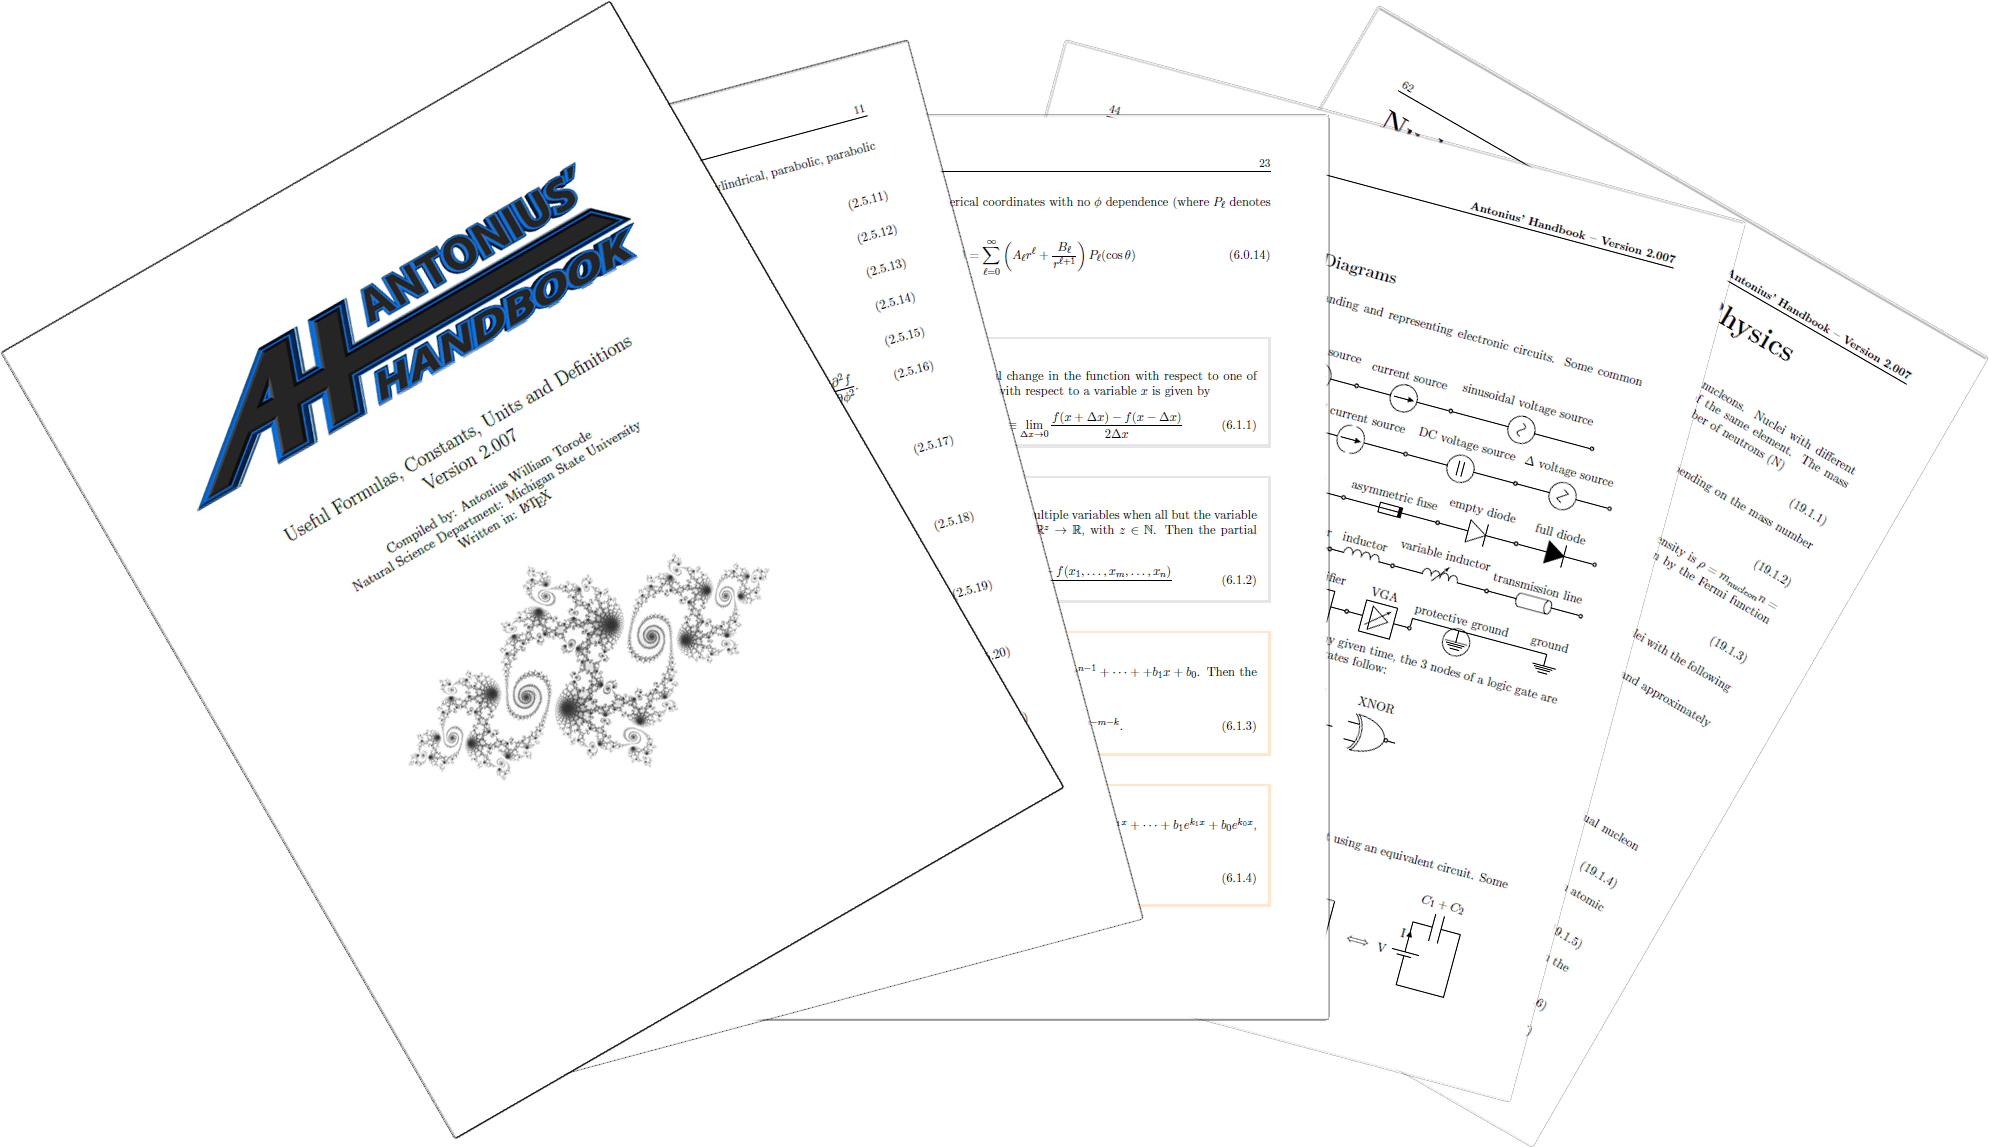
\includegraphics[scale=.4]{./Images/Covers/background.png}
\end{center}

%Copywrite page
\pagestyle{empty}
%% copyrightpage
\begingroup
\footnotesize
\parindent 0pt
\parskip \baselineskip
\textcopyright{} 2016 Antonius Torode \\
All rights reserved.

This work may be distributed and/or modified under the conditions of the Antonius' Handbook License.

The original maintainer of this work is: Antonius Torode.

The current maintainer of this work is: Antonius Torode.

Published by Antonius Torode. 

Hosted at: https://msu.edu/{\raise.17ex\hbox{$\scriptstyle\sim$}}torodean/AHandbook.html

Github Repository: https://github.com/torodean/Antonius-Handbook

\begin{center}
\begin{tabular}{ll}
First Personal Release (Version 0.000): & January 2016 \\
First Public Release (Version 1.000): &  July 2016 \\
Most Current Revision Date (Version 2.000+): & \today 
\end{tabular}
\end{center}

\vfill

Torode, A.\\
\hspace*{2em} Michigan State University -- \\
\hspace*{1em} Department of Physics \& Astronomy. \\
\hspace*{2em} 2016, Student. \\
\hspace*{2em} Version: \Version \\
\hspace*{2em} Includes References \\
\hspace*{2em} ISBN: NONE



\endgroup
\clearpage

%Preface page
\begin{center}
	\textbf{Preface}
\end{center}

This document is a compilation of useful formulas, definitions, constants, and general information used throughout my own schooling as a reference while furthering education. It's purpose is to provide a complete 'encyclopedia' per say of various mathematical and significant ideas used often. The idea and motivation behind it is to be a quick reference providing easily accessible access to necessary information for either double checking or recalling proper formula for use in various situations due to my own shortcomings in matters of memorization. All the material in this document was either directly copied from one of the references listed at the end or derived from scratch. On occasion typos may exist due to human error but will be corrected when discovered.
	
The version number is updated every time the document is distributed, printed, or referred to. This ensures that there is no two copies with different information and similar version numbers. The latest update date is automatically set to the current date each time the document is edited. Please refrain from distributing this handbook without permission from the original author/compiler. As of version 1.035 this book is formatted for printing.

\begin{center}
	\textbf{Courses Covered In This Book}
\end{center}

This document encompasses a large portion of formula used throughout specific courses at Michigan state University. The courses which have information pertaining to something in this book are more than just listed below; however, below is a list of classes that the author took whilst compiling the information in this book. All course numbers correspond to Michigan State University courses at the time of adding them. 

\begin{multicols}{2}
\begin{itemize}
	\item AST 207/208/304: Astrophysics I/II/III
	\item PHY 215: Thermodynamics \& Modern Physics
	\item MTH 310: Abstract Algebra/Number Theory
	\item PHY 321: Classical Mechanics I
	\item PHY 410: Thermal \& Statistical Physics
	\item PHY 415: Methods Of Theoretical Physics
	\item PHY 440: Electronics
	\item PHY 471/472: Quantum Physics I/II
	\item PHY 481/482: Electricity and Magnetism I/II
	\item PHY 492: Introduction to Nuclear Physics
\end{itemize} 
\end{multicols}

The information in this book is in no way limited to the material used within the courses above. They serve as a simple guideline to what you will find within this document. For more information about this book or details about how to obtain your own copy please visit:
\begin{center}
	https://msu.edu/{\raise.17ex\hbox{$\scriptstyle\sim$}}torodean/AHandbook.html
\end{center}
\begin{center}
	\textbf{Disclaimer}
\end{center}

This book contains formulas, definitions, and theorems that by nature are very precise. Due to this, some of the material in this book was taken directly from other sources such as but not limited to Wolfram Mathworld. This is only such in cases where a change in wording could cause ambiguities or loss of information quality.  Following this, all sources used are listed in the references section.

%Begins blank page.
\thispagestyle{empty}
\newpage
\vspace*{\stretch{1}}
\begin{center}
	\textit{This page intentionally left blank.\\ (Yes, this is a contradiction.)}
\end{center}
\vspace*{\stretch{1}}

%Begins table of contents
\tableofcontents


%Begin the mainmatter.
\setlength{\parindent}{0pt}
\mainmatter
\pagestyle{fancy}
\chapter{Constants and units}
\thispagestyle{fancy}
\begin{fancybox}[Physical Constants]{}	
\begin{center}
	\begin{tabular}{   l  |  c  |  l  |  l  }
		Constant & Symbol & Value & Units \\
		\hline
		Speed of light in a vacuum& c & $2.99792458 \times 10^8$ & m/s \\
		Elementary charge& e & $1.602176565(35)\times 10^{-19}$ & C\\
		Gravitational constant& G & $6.67384(80)\times 10^{-11}$ & m$^3$kg$^{-1}$s$^{-2}$\\
		Avagadro's number& $N_a$ & $6.02214129(27)\times 10^{23}$ & mol$\cdot s^{-1}$\\
		Planck constant & $h$ & $ 6.62606872(52) \times 10^{-34}$ & J$\cdot$s \\
		& & $4.135668 \times 10^{-15}$ & eV$\cdot$s \\
		& $hc$ & 1239.84 & eV$\cdot$nm \\
		Reduced planck constant& $\hbar \equiv h/2\pi$ & $1.05\times 10^-{34}$ & J$\cdot$s\\
		Permittivity of the vacuum & $\epsilon_0$ & $8.854\times 10^{-12}$ & C$^2$N$^{-1}$m$^{-2}$ \\
		Permeability of the vacuum & $\mu_0$ & $4\pi\times 10^{-7}$ & W$\cdot$m \\
		Boltzmann constant & k & $1.38064852\times 10^{-23}$ & J/K \\
				 & & $8.61733\times 10^{-5}$ & eV/K \\
		Stefan-Boltzmann constant & $\sigma_{\textrm{SB}}$ & $5.670367(13)\times 10^{-8}$ & W$\cdot$m$^{-2}$K$^{-4}$ \\
		Thomson cross-section & $\sigma_e$ & $6.652\times10^{-29}$ & $m^2$ \\
		The Bohr Magneton & $\mu_B \equiv \frac{e\hbar}{2m}$ & $5.788\times 10^{-5}$ & eV/T \\
		& & $9.274\times 10^{-24}$ & Am$^2$ \\
		Mass of an electron & $m_e$ & $9.10938291(40)\times 10^{-31}$ & kg\\
		&  & $510.9989$ & keV/$c^2$\\
		Mass of a proton& $m_p$ & $1.6726218 \times 10^{-27}$ & kg\\
		&  & 938.27203 & MeV/$c^2$\\
		Mass of a neutron& $m_n$   & $1.6749274 \times 10^{-27}$ & kg \\
		& & $939.56536$ & MeV/$c^2$	\\
		Unified amu & $u$ &  $1.660538782\times 10^{-27}$ & kg \\
		  &   &  931.494028 & MeV/c$^2$ 
	\end{tabular}
\end{center}
\end{fancybox}

\begin{fancybox}[Stellar Data]{}
	\begin{center}
		\begin{tabular}{c|c|c|c|c|c}
			Spectral Type & $T_{eff}$ (K) & $M/M_\cdot$ & $L/L_\cdot$ & $R/R_\cdot$ & $V_{mag}$ \\
			\hline
			O5 & 44,500 & 60 & $7.9\times 10^5$ & 12 &-5.7 \\
			B5 & 15,400 & 5.9 & 830 & 3.9 & -1.2 \\
			A5 & 8,200 & 2.0 & 14 & 1.7 & 1.9 \\
			F5 & 6,440 & 1.4 & 3.2 & 1.3 & 3.4 \\
			G5 & 5,770 & 0.92 & 0.79 & 0.92 & 4.9 \\
			K5 & 4,350 & 0.67 & 0.15 & 0.72 & 6.7 \\
			M5 & 3,170 & 0.21 & 0.011 & 0.27 & 12.3 \\
		\end{tabular}
	\end{center}
\end{fancybox}



\newpage
\begin{fancybox}[Astronomical Constants]{1}
\begin{center}
\begin{tabular}{   l  |  c  |  l  |  l  }
Constant & Symbol & Value & Units \\
\hline
Mass of Earth& $M_\oplus$ & $5.974 \times 10^{24}$ & kg\\
Mass of Sun& $M_\odot$ &$1.989  \times 10^{30}$ & kg\\
Mass of Moon& $M_{\leftmoon}$ &$7.36 \times 10^{22}$&  kg\\
Equatorial radius of Earth& $R_\oplus$ & $6.378 \times 10^6$& m\\
Equatorial radius of Sun& $R_\odot$ &$6.6955 \times 10^8$ & m\\
Equatorial radius of Moon& $R_{\leftmoon}$ &$1.737 \times 10^{6}$ & m\\
Mean density of Earth &  & 5515  & kg$\cdot$m$^{-3}$  \\
Mean density of Sun &  & 1408  & kg$\cdot$m$^{-3}$ \\
Mean density of Moon  & & 3346  & kg$\cdot$m$^{-3}$ \\
Earth-Moon distance& &$3.84 \times 10^8$ & m\\
Earth-Sun distance& &$1.496 \times 10^{11}$ & m \\
Luminosity of Sun & $L_\odot$  & $3.839\times 10^{26}$  & W  \\
Effective temp. of Sun &   & 5778  & K  \\
Hubble constant & $H_0$  & $70\pm 5$  & km$\cdot$s$^{-1}$Mpc$^{-1}$  \\
Parsec& pc & 206264.81 & AU\\
&  & $3.0856776 \times 10^{16}$ & m\\
& & $3.2615638$ & ly \\
Astronomical Unit & AU & $1.496 \times 10^{11}$ & m \\
Light year& ly & $9.461 \times 10^{15}$ & m \\
1 year on Earth& yr & 365.25 & days \\
&  & $3.15576 \times 10^{7}$& s 
\end{tabular}
\end{center}
\end{fancybox}

\begin{fancybox}[Solar System]{}
	\begin{center}
		\begin{tabular}{   l  |  c  |  l  |  l  | l}
			Planet & Symbol & Mass (kg) & Radius (m) & Sun-Distance (km) \\
			\hline
			Mercury & \mercury & $3.285 \times 10^{23}$ & 2.44 $\times 10^{6}$ & $5.791 \times 10^{10}$ \\
			Venus & \venus & $4.867 \times 10^{24}$ & $6.052 \times 10^{6}$ & $1.082 \times 10^{11}$   \\
			Mars & \mars & $6.39 \times 10^{23}$ & $3.390 \times 10^{6}$ & $2.279 \times 10^{11}$ \\
			Jupiter& \jupiter &$1.898 \times 10^{27}$ & $3.83 \times 10^{11}$ & $7.785 \times 10^{11}$  \\
			Saturn & \saturn & $5.683 \times 10^{26}$ & $5.8232 \times 10^{7}$ & $1.429 \times 10^{12}$  \\
			Uranus & \uranus & $8.681 \times 10^{25}$ & $2.5362 \times 10^{7}$ & $2.871 \times 10^{12}$  \\
			Neptune & \neptune & $1.024 \times 10^{26}$ & $2.4622 \times 10^{7}$ & $4.498 \times 10^{12}$  \\
			Pluto & \pluto & $1.309 \times 10^{22}$ & $1.187 \times 10^6$ & $5.906 \times 10^{12}$ 
		\end{tabular}
	\end{center}
\end{fancybox}

\newpage
\begin{fancybox}[Unit conversions]{}
	The International System of Units (SI) defines seven units of measure as a basic set from which all other SI units can be derived. These are [length](m), [time](s), [mass](kg), [electric current] $\equiv$ [Ampere](A), [temperature](K), [luminous intensity](cd), [amount of substance](mol).
	\begin{center}
		\begin{tabular}{c|l|l}
			Unit Symbol & Unit & Equivalence \\
			\hline
			C & [Coulomb] & [Ampere][time] \\
			N & [Newton] & [mass][length][time]$^{-2}$ \\
			P & [Pascal]  & [mass][length]$^{-1}$[time]$^{-2}$ \\
			J & [Joule]  & [mass][length]$^{2}$[time]$^{-2}$ \\
			W & [Watt]  & [mass][length]$^{2}$[time]$^{-3}$ \\
			 & & [Ohm][Ampere]$^2$ \\
			 & & [Volt]$^2$[Ohm]$^{-1}$ \\
			V & [Volt]  & [mass][length]$^{2}$[time]$^{-3}$[Ampere]$^{-1}$ \\
			Wb & [Weber]  & [mass][length]$^{2}$[time]$^{-2}$[Ampere]$^{-1}$ \\
			T & [Tesla]  & [mass][time]$^{-2}$[Ampere]$^{-1}$ \\
			H & [henry]  & [mass][length]$^{2}$[time]$^{-2}$[Ampere]$^{-2}$ \\
			$\Omega$ & [Ohm]  & [mass][length]$^{2}$[time]$^{-3}$[Ampere]$^{-2}$ \\
			F & [Farad]  & [mass]$^{-1}$[length]$^{-2}$[time]$^{4}$[Ampere]$^{2}$ \\
			Hz & [Hertz]  & [time]$^{-1}$ 
		\end{tabular}
	\end{center}
\end{fancybox}


\begin{fancybox}[Number Sets ($i \equiv \sqrt{-1}$)]{}
	\begin{center}
		\begin{tabular}{c|l||c|l}
			Symbol &  Set  & Symbol & Set   \\
			\hline
			$\mathbb{R}$ & Real numbers & $\emptyset$ & \{\} \\
			$\mathbb{N}\equiv \mathbb{N}_1$ & \{1,2,3,4,\dots\} & $\mathbb{Z}$ & \{\dots,-2,1,0,1,2,\dots\} \\
			$\mathbb{Z}^+ \equiv \mathbb{N}_0$ & \{0,1,2,3,\dots\} & $\mathbb{Z}^-$ & \{0,-1,-2,-3,-4,\dots\} \\
			$\mathbb{C}$ & $\{x+iy | x,y \in \mathbb{R}\}$ & $\mathbb{Q}$ & $\{\frac{x}{y} | x,y \in \mathbb{Z}\}$ \\
			$\mathbb{I}$ & $\{ix|x\in \mathbb{R}\}$ & $\mathbb{U}$ & Universal Set \footnote{Definition: The set containing all objects or elements and of which all other sets are subsets.} \\
			$\mathbb{A}$ & Algebraic Numbers\footnote{Any number that is a solution to a polynomial equation with rational coefficients.} & $\mathbb{T}$ & Transcendental Numbers \footnote{Any number that is not an Algebraic Number.} 
		\end{tabular}
	\end{center}
\end{fancybox}



\newpage
\chapter{General Mathematics}
\thispagestyle{fancy}
Definitions
\begin{multicols}{2}
	\noindent
	\begin{align}
	\sin(x) &=\frac{1}{2i}(e^{ix}-e^{-ix}) \\
	\sinh(x) &= \frac{1}{2}(e^{x}-e^{-x}) \\
	&= -i\sin(ix)
	\end{align}
	\begin{align}
	\cos(x) &=\frac{1}{2}(e^{ix}+e^{-ix}) \\
	\cosh(x) &=\frac{1}{2}(e^{x}+e^{-x}) \\
	&= \cos(ix)
	\end{align}
\end{multicols}
\textbf{Curl Theorem:}\index{Curl Theorem} A special case of Stokes' theorem\index{Stokes' theorem} in which $\vec{F}$ is a vector field and $M$ is an oriented, compact embedded 2-manifold with boundary in $\mathbb{R}^3$, and a generalization of Green's theorem from the plane into three-dimensional space. The curl theorem states 
\begin{align}
	\int_S (\nabla \times \vec{F})\cdot d\vec{a} = \int_{\partial S}\vec{F} \cdot d\vec{s}
\end{align}
\textbf{Green's theorem}\index{Green's theorem} is a vector identity which is equivalent to the curl theorem 
\begin{align}
	\iint_S \left(\frac{\partial Q}{\partial x}-\frac{\partial P}{\partial y}\right) dxdy = \oint_{\partial S} P(x,y)dx+Q(x,y)dy
\end{align}
The \textbf{divergence theorem}\index{Divergence theorem} is also known as Gauss's theorem (e.g., Arfken 1985) or the Gauss-Ostrogradsky theorem. Let $V$	 be a region in space with boundary $\partial V$. Then the volume integral of the divergence $\nabla \cdot \vec{F}$ of $\vec{F}$ over $V$ and the surface integral of $\vec{F}$ over the boundary $\partial V$ of $V$ are related by 
\begin{align}
	\int_V (\nabla \cdot \vec{F}) dV = \int_{\partial V}\vec{F} \cdot d\vec{a}
\end{align}
The \textbf{gradient theorem}\index{Gradient theorem} (where the integral is a line integral) is
\begin{align}
	\int_a^b (\nabla f) \cdot d\vec{s} = f(b)-f(a)
\end{align}
The \textbf{Gamma function}\index{Gamma function} $\Gamma$ and the \textbf{Riemann zeta function} $\zeta$ are given by
\begin{align}
\Gamma(z) &\equiv\int_{0}^{\infty}t^{z-1}e^{-t}dt \\
\zeta(z)&=\sum_{k=1}^{\infty}\frac{1}{k^z}\implies \zeta'(z)=-\sum_{k=1}^{\infty}\frac{\ln(k)}{k^z} \\
\zeta(z)\Gamma(z)&=\int_{0}^{\infty}\frac{u^{z-1}}{e^u-1}du
\end{align}
The most general case of the \textbf{binomial theorem} \index{Binomial theorem} is the binomial series identity 
\begin{align}
(x+y)^n &= \sum_{i=1}^{n} {{n}\choose{k}}x^{n-k}y^{k}
\end{align}
The \textbf{binomial coefficient} is defined as follows, with Pascals Formula implied.
\begin{align}
_nC_r\equiv{{n}\choose{k}} &\equiv \frac{n!}{(n-k)!k!} \equiv \frac{\Gamma(n+1)}{\Gamma(k+1)\Gamma(n-k+1)} \\
{{n}\choose{k}}&={{n-1}\choose{k-1}}+{{n-1}\choose{k}}
\end{align}
The general formula for the power sum of the first $n$ positive integers, 
\begin{align}
\sum_{k=1}^{n}k^p=\frac{1}{p+1}\sum_{i=1}^{p+1}(-1)^{\delta_{ip}}{{p+1}\choose{i}}B_{p+1-i}n^i,
\end{align}
where $\delta_{ip}$ is the Kronecker delta  and $B_i$ is the $i$th Bernoulli number. The Bernoulli numbers $B_n$ are a sequence of signed rational numbers that can be defined by the exponential generating function 
\begin{align}
\frac{x}{e^x-1}\equiv\sum_{n=0}^{\infty}\frac{B_nx^n}{n!}.
\end{align}
The simplest interpretation of the \textbf{Kronecker delta}\index{Kronecker delta} is as the discrete version of the delta function defined by 
\begin{align}
\delta_{ij}\equiv
\begin{cases}
0 & \textrm{for } i \neq j \\
1 & \textrm{for } i = j.
\end{cases}
\end{align}
Determining the sums for the first few terms of the power sum give
\begin{align}
\sum_{i=0}^{n}i   &=\frac{1}{2}n(n+1) \\
\sum_{i=0}^{n}i^2 &=\frac{1}{6}(2n^3+3n^2+n)=\frac{1}{6}n(2n+1)(n+1) \\
\sum_{i=0}^{n}i^3 &=\frac{1}{4}(n^4+2n^3+n^2)=\frac{1}{4}n^2(n+1)^2 \\
\sum_{i=0}^{n}i^4 &=\frac{1}{30}(6n^5+15n^4+10n^3-n) \\
\sum_{i=0}^{n}i^5 &=\frac{1}{12}(2n^6+6n^5+5n^4-n^2).
\end{align}
A \textbf{Taylor series}\index{Taylor series} is an expansion of a function about a point. A one-dimensional Taylor series of a real function $f(x)$ about the point x=a is given by 
\begin{align}
f(x)&=f(a)+f'(a)(x-a)+\frac{1}{2!}f''(a)(x-a)^2+\frac{1}{3!}f'''(a)(x-a)^4+\cdots 
\end{align}
Some common series expansions include: 
\begin{align}
e^x&=\sum_{n=0}^{\infty} \frac{x^n}{n!}=1+x+\frac{1}{2!}x^2 +\frac{1}{3!}x^3 +\cdots \\ 
\ln(1+x)&=\sum_{n=0}^{\infty} \frac{(-1)^{n}x^{n+1}}{n+1}=x-\frac{1}{2}x^2 +\frac{1}{3}x^3 -\cdots\hspace{0.5cm} \textrm{with }|x|<1\\ 
\sin(x)&=\sum_{n=0}^{\infty}\frac{(-1)^{n}x^{2n+1}}{(2n+1)!} = x-\frac{x^3}{3!}+\frac{x^5}{5!}-\cdots \\
\cos(x)&=\sum_{n=0}^{\infty}\frac{(-1)^{n}x^{2n}}{(2n)!} = 1-\frac{x^2}{2!}+\frac{x^4}{4!}-\cdots \\
\tan(x)&= x+\frac{1}{3}x^3+\frac{2}{15}x^5+\cdots[|x|<\pi/2] \\
\sinh(x)&=\sum_{n=0}^{\infty}\frac{x^{2n+1}}{(2n+1)!} = x+\frac{x^3}{3!}+\frac{x^5}{5!}+\cdots \\
\cosh(x)&=\sum_{n=0}^{\infty}\frac{x^{2n}}{(2n)!} = 1+\frac{x^2}{2!}+\frac{x^4}{4!}+\cdots \\
\tanh(x)&= x-\frac{1}{3}x^3+\frac{2}{15}x^5-\cdots[|x|<\pi/2]\\
(1+x)^n&=1+nx+\frac{n(n-1)}{2!}x^2+\cdots[|x| < 1]
\end{align}	
\textbf{Dirac Delta Function:}\index{Dirac Delta Function} The delta function is a generalized function that can be defined as the limit of a class of delta sequences.
\begin{align}
	\delta(x) = \frac{1}{\pi}\lim_{\epsilon\rightarrow 0}\frac{\epsilon}{x^2+\epsilon^2} = \frac{1}{2}\lim_{\epsilon\rightarrow 0}\epsilon|x|^{\epsilon-1} =\lim_{\epsilon\rightarrow 0} \frac{1}{\pi x}\sin\left(\frac{x}{\epsilon}\right) = \lim_{\epsilon\rightarrow 0^+}\frac{1}{2\sqrt{\pi \epsilon}}e^{-x^2/(4\epsilon)}
\end{align}
The Dirac delta can be thought of as a function on the real line which is zero everywhere except where the arguments of the function are zero, where it is infinite,
\begin{align}
	\delta(x) = 
	\begin{cases} 
		\infty & x=0 \\
			 0 & x \neq 0 
	\end{cases}
\end{align}
For any $\epsilon > 0$, the delta function has the fundamental property that 
\begin{align}
	\int_{-\infty}^{\infty}f(x)\delta(x-a)dx = f(a) \hspace{1cm}\textrm{and}\hspace{1cm}\int_{x-\epsilon}^{x+\epsilon}f(x)\delta(x-a)dx = f(a)
\end{align}
The fundamental equation that defines derivatives of the delta function $\delta(x)$ is
\begin{align}
	\int f(x)\delta^{(n)}(x)dx \equiv -\int \frac{\partial f}{\partial x}\delta^{(n-1)}(x)dx
\end{align} 
This implies 
\begin{align}
	x^n\delta^{(n)}(x)=(-1)^nn!\delta(x)
\end{align}
A few identities and common expressions using the delta function are
\begin{align}
	\int_{-\infty}^{\infty}f(x)\delta(ax)dx &= \frac{1}{|a|}f(0) \\
	\int_{-1}^{1}\delta\bigg(\frac{1}{x}\bigg)dx = 0
\end{align}



\section{Coordinate Systems}
\begin{multicols}{2}
Cylindrical coordinates\index{Cylindrical coordinates}
\begin{align}
r&=\sqrt{x^2+y^2} \\
x&=r\cos(\theta) \\
y&=r\sin(\theta) \\
z&=z \\
dV&= r \textrm{ dr d$\theta$ dz}
\end{align}
Spherical coordinates\index{Spherical!coordinates}
\begin{align}
r&=\sqrt{x^2+y^2+z^2} \\
x&=r\sin(\theta)\cos(\phi) \\
y&=r\sin(\theta)\sin(\phi) \\
z&=r\cos(\theta) \\
dV&=r^2\sin(\theta)\textrm{dr d$\theta$ d$\phi$}
\end{align}
Polar Coordinates\index{Polar Coordinates}
\begin{align}
	r&=\sqrt{x^2+y^2} \\
	x&=r\cos(\theta) \\
	y&=r\sin(\theta) \\
	dA&= r \textrm{ dr d$\theta$}
\end{align}
Elliptic cylindrical coordinates\index{Elliptic cylindrical coordinates}
\begin{align}
	x&= a \cosh(u) \cos(v) \\
	y&= a \sinh(u) sin(v) \\
	z&= z \\
	dV&=a^2[\sinh^2(u)+\cosh^2(v)]\textrm{du dv dz}
\end{align}
\end{multicols}

\section{Vector Operations}
For any vector $\vec{r}=(r_1,r_2,\dots,r_n)$ in $n$-dimensions, the magnitude and unit vector is
\begin{align}
|\vec{r}|\equiv\sqrt{\vec{r}\cdot\vec{r}}=\sqrt{r_1^2+r_2^2+\cdots+r_n^2} \hspace{2cm} \hat{r}\equiv\frac{\vec{r}}{|\vec{r}|}
\end{align}
Dot and cross products for 3-dimensional vectors, where $\theta$ is the smallest angle between them, $\vec{r}=(r_x,r_y,r_z)$ and $\vec{s}=(s_x,s_y,s_z)$
\begin{align}
\vec{r}\cdot \vec{s} &=|\vec{r}||\vec{s}|\cos(\theta)=r_xs_x+r_ys_y+r_zs_z \\
\vec{r} \times \vec{s} &= |\vec{r}||\vec{s}|\sin(\theta)= (r_ys_z-r_zs_y, r_zs_x-r_xs_z, r_xs_y-r_ys_x) =  \begin{vmatrix}
\boldsymbol{\hat{x}} & \boldsymbol{\hat{y}} & \boldsymbol{\hat{z}} \\ 
r_x & r_y & r_z \\ 
s_x & s_y & s_z 
\end{vmatrix}
\end{align}
Triple product vector identities
\begin{align}
\vec{A}\cdot (\vec{B} \times \vec{C}) = \vec{B}\cdot (\vec{C}\times \vec{A})= \vec{C}\cdot(\vec{A}\times \vec{B}) &= -\vec{B}\cdot (\vec{A} \times \vec{C}) = -\vec{C}\cdot (\vec{B} \times \vec{A})=-\vec{A}\cdot (\vec{C} \times \vec{B}) \\
\vec{A}\times (\vec{B}\times \vec{C}) &=\vec{B}(\vec{A}\cdot\vec{C})-\vec{C}(\vec{A}\cdot\vec{B})
\end{align}
Product rule vector identities
\begin{align}
	\nabla (fg) &= f(\nabla g) + g(\nabla f) \\
	\nabla (\vec{A} \cdot \vec{B}) &= \vec{A} \times(\nabla \times \vec{B})+ \vec{B} \times (\nabla \times \vec{A}) + (\vec{A} \cdot \nabla)\vec{B} + (\vec{B} \cdot \nabla)\vec{A} \\
	\nabla \cdot (f\vec{A}) &= f(\nabla  \cdot \vec{A}) + \vec{A} \cdot (\nabla f) \\
	\nabla \cdot (\vec{A} \times \vec{B}) &= \vec{B} \cdot (\nabla \times \vec{A}) - \vec{A} \cdot (\nabla \times \vec{B}) \\
	\nabla \times (f\vec{A}) &= f(\nabla \times \vec{A})- \vec{A} \times (\nabla f) \\
	\nabla \times (\vec{A}\times\vec{B}) &= (\vec{B}\cdot \nabla)\vec{A}-(\vec{A}\cdot\nabla)\vec{B}+\vec{A}(\nabla \cdot \vec{B})-\vec{B}(\nabla\cdot\vec{A})
\end{align}
Second derivative vector identities
\begin{align}
	\nabla \cdot (\nabla \times \vec{A}) =0 \hspace{2cm} \nabla \times (\nabla f)=0 \hspace{2cm}
	\nabla \times (\nabla \times \vec{A}) = \nabla (\nabla \cdot \vec{A})- \nabla^2\vec{A}
\end{align}
A few other useful identities include
\begin{align}
	\nabla \cdot \frac{\hat{r}}{r^2} = 4\pi\delta^2(\vec{r}) \hspace{2cm}\nabla \times \frac{\hat{r}}{r^2} =\frac{\vec{r}}{r^3}= 0 \hspace{2cm} \nabla \cdot \frac{\hat{r}}{r} = \frac{1}{r^2}
\end{align}

\section{Triangles}
Let a triangle have side lengths $a$, $b$, and $c$ with opposite angles $A$, $B$, and $C$. 
\begin{multicols}{2}
The area of a triangle can be given by 
\begin{align}
A&=\sqrt{s(s-a)(s-b)(s-c)} \\
s&=(a+b+c)/2
\end{align}		
Law of Cosines:\index{Law of Cosines}
\begin{align}
c^2=a^2+b^2-2ab\cos(C)
\end{align}
Law of Sines:\index{Law of Sines}
\begin{align}
\frac{\sin(A)}{a}=\frac{\sin(B)}{b}=\frac{\sin(C)}{c}
\end{align}
Law of tangents:\index{Law of tangents}
\begin{align}
\frac{a-b}{a+b}=\frac{\tan((A-B)/2)}{\tan((A+B)/2)}
\end{align}
\end{multicols}
Mollweide's Formulas:\index{Mollweide's Formulas:}
\begin{align}
\frac{b-c}{a} &=\frac{\sin[(B-C)/2]}{\cos(A/2)} \\
\frac{c-a}{b} &=\frac{\sin[(C-A)/2]}{\cos(B/2)} \\
\frac{a-b}{c} &=\frac{\sin[(A_B)/2]}{\cos(C/2)}
\end{align}	

\newpage

\section{Trigonometric Identities}\index{Trigonometric Identities}
\begin{multicols}{2}
Pythagorean identities:
\begin{align}
1 &= \sin^2(\theta)+\cos^2(\theta)\\
1 &= \sec^2(\theta)-\tan^2(\theta) \\
1 &= \csc^2(\theta)-\cot^2(\theta) \\
1 &= \cosh^2(\theta)-\sinh^2(\theta) \\
1 &= \textrm{sech}^2(\theta)+\tanh^2(\theta)
\end{align}
Sum-Difference Formulas:
\begin{align}
\sin(\theta \pm \phi) &= \sin(\theta)\cos(\phi)\pm \cos(\theta)sin(\phi) \\
\cos(\theta \pm \phi) &= \cos(\theta)\cos(\phi)\mp \sin(\theta)sin(\phi) \\
\tan(\theta \pm \phi) &= \frac{\tan(\theta)\pm \tan (\phi)}{1 \mp \tan(\theta)\tan(\phi)}
\end{align}
Double Angle formulas:
\begin{align}
\sin(2\theta) &= 2\sin(\theta)\cos(\theta) \\
\cos(2\theta) &= \cos^2(\theta)-\sin^2(\theta)\\
&= 2\cos^2(\theta)-1 \\
&= 1 - 2\sin^2(\theta) \\
\tan(2\theta) &= \frac{2 \tan(\theta)}{1-\tan^2(\theta)}
\end{align}
Power-Reducing/Half Angle Formulas:
\begin{align}
\sin^2(\theta) &= \frac{1-\cos(2\theta)}{2}\\
\cos^2(\theta) &= \frac{1+\cos(2\theta)}{2}\\
\tan^2(\theta) &= \frac{1-\cos(2\theta)}{1+\cos(2\theta)}
\end{align}
Phase changes follow:
\begin{align}
\sin(-\theta) &=-\sin(\theta) \\
\cos(-\theta) &= \cos(\theta) \\
\sin(\theta\pm \pi/2) &= \pm \cos(\theta) \\
\sin(\theta\pm \pi) &= - \sin(\theta) \\
\cos(\theta\pm \pi/2) &= \mp \sin(\theta) \\
\cos(\theta\pm \pi) &= - \cos(\theta) 
\end{align}
Half-angle formulas
\begin{align}
\sin\bigg(\frac{\theta}{2}\bigg)=(-1)^{\theta/(2\pi)}\sqrt{\frac{1-\cos(\theta)}{2}} \\
\cos\bigg(\frac{\theta}{2}\bigg)=(-1)^{(\theta+\pi)/(2\pi)}\sqrt{\frac{1+\cos(\theta)}{2}}
\end{align}
The \textbf{Weierstrass substitution}\index{Weierstrass substitution} makes use of the half-angle formulas 
\begin{align}
\cos(\theta)=\frac{1-\tan^2(\theta/2)}{1+\tan^2(\theta/2)} \\
\sin(\theta)=\frac{2\tan(\theta/2)}{1+\tan^2(\theta/2)}
\end{align}
Other relations and identities:
\begin{align}
	\cos(x)\cos(y) &= \frac{1}{2}[\cos(x-y)+\cos(x+y)] \\
	\sin(x)\sin(y) &= \frac{1}{2}[\cos(x-y)-\cos(x+y)]
\end{align}
\end{multicols}
The half angle identity for tangent.
\begin{align}
\tan\bigg(\frac{\theta}{2}\bigg)=(-1)^{x/\pi}\sqrt{\frac{1-\cos(\theta)}{1+\cos(\theta)}} = \frac{\sin(\theta)}{1+\cos(\theta)}=\frac{1-\cos(\theta)}{\sin(\theta)}=\frac{\tan(\theta)\sin(\theta)}{\tan(\theta)+\sin(\theta)}
\end{align}

Multiple-angle formulas are given by 
\begin{align}
\sin(nx)&= \sum_{k=0}^{n}{{n}\choose{k}}\cos^k(x)\sin^{n-k}(x)\sin\big((n-k)\pi/2 \big) \\
\cos(nx)&= \sum_{k=0}^{n}{{n}\choose{k}}\cos^k(x)\sin^{n-k}(x)\cos\big((n-k)\pi/2 \big)
\end{align}

Other identities
\begin{align}
\cos(\theta)cos(\phi) &=\frac{1}{2}[\cos(\theta+\phi)+\cos(\theta-\phi)] \\
\sin(\theta)sin(\phi) &=\frac{1}{2}[\cos(\theta-\phi)-\cos(\theta+\phi)] \\
\sin(\theta)cos(\phi) &=\frac{1}{2}[\sin(\theta+\phi)+\sin(\theta-\phi)] \\
\cos(\theta)+\cos(\phi)&= 2\cos\bigg( \frac{\theta+\phi}{2}\bigg)\cos\bigg( \frac{\theta-\phi}{2}\bigg) \\
\cos(\theta)-\cos(\phi)&= 2\sin\bigg( \frac{\theta+\phi}{2}\bigg)\sin\bigg( \frac{\theta-\phi}{2}\bigg)
\end{align}



\section{Arbitrary Orthogonal Curvilinear Coordinates}\index{Orthogonal Coordinates}
A coordinate system composed of intersecting surfaces. If the intersections are all at right angles, then the curvilinear coordinates are said to form an orthogonal coordinate system. The scale factors are $h_i$,
\begin{align}
	\vec{a}_i &\equiv\frac{\partial \vec{r}}{\partial e_i} =  \frac{\partial x}{\partial e_i} \hat{x} + \frac{\partial y}{\partial e_i}\hat{y} + \frac{\partial x}{\partial e_i} \hat{z} = h_i \hat{e}_i = |\vec{a}_i| \hat{e}_i \\
	h_i &\equiv \left|\frac{\partial \vec{r}}{\partial e_i}\right|=|\vec{a}_i| = \sqrt{\frac{\partial x}{\partial e_i}+\frac{\partial y}{\partial e_i}+\frac{\partial z}{\partial e_i} } \\ \hat{e}_i &= \frac{1}{h_1}\frac{\partial \vec{r}}{\partial e_i}=\frac{\vec{a}_i}{|\vec{a}_i|}
\end{align}
The line element $d\vec{s}$ is determined by
\begin{align}
	d\vec{s}\equiv 
	d\vec{x}+d\vec{y}+d\vec{z} \equiv
	\vec{a}_1de_1+\vec{a}_2de_2+\vec{a}_3de_3
\end{align}
From this, $ds^2$ is given by
\begin{align}
	ds^2= d\vec{s}\cdot d\vec{s} = dx^2+dy^2+dz^2= h_1^2de_1^2+h_2^2de_2^2+h_3^2de_3^2
\end{align}
The differential vector and volume elements are therefore
\begin{align}
	d\vec{r} &= h_1 du_1 \hat{u}_1+h_2 du_2 \hat{u}_2+h_3 du_3 \hat{u}_3 \\
	dV &=h_1h_2h_3 du_1du_2du_3 = \left|\frac{\partial(x,y,z)}{\partial(u_1,u_2,u_3)}\right|du_1du_2du_3
\end{align}
The gradient in arbitrary curvilinear coordinates such that the gradient theorem is preserved:
\begin{align}
	\nabla f = \frac{1}{h_1}\frac{\partial f}{\partial x_1}\hat{x}_1+\frac{1}{h_2}\frac{\partial f}{\partial x_2}\hat{x}_2+\frac{1}{h_3}\frac{\partial f}{\partial x_3}\hat{x}_3
\end{align}
The divergence in arbitrary curvilinear coordinates such that the divergence theorem is preserved:
\begin{align}
	\nabla \cdot \vec{v} = \frac{1}{h_1h_2h_3}\left[\frac{\partial v_1}{\partial x_1}h_2h_3+\frac{\partial v_2}{\partial x_2}h_1h_3+\frac{\partial v_3}{\partial x_3}h_1h_2\right]
\end{align}
The Laplacian\index{Laplacian} for a scalar function $\phi$ (where the $h_i$ are the scale factors of the coordinate system - Weinberg 1972, p. 109; Arfken 1985, p. 92 \cite{bib:Wolfram}) is a scalar differential operator defined by
\begin{align}
	\nabla^2 \phi = \frac{1}{h_1h_2h_3} \bigg[	\frac{\partial}{\partial u_1} \bigg( \frac{h_2h_3}{h_1} \frac{\partial}{\partial u_1} \bigg) + \frac{\partial}{\partial u_2} \bigg( \frac{h_1h_3}{h_2} \frac{\partial}{\partial u_2} \bigg) + \frac{\partial}{\partial u_3} \bigg( \frac{h_1h_2}{h_3} \frac{\partial}{\partial u_3} \bigg) \bigg] \phi
\end{align}
The form of the Laplacian in several common coordinate systems (cartesian, cylindrical, parabolic, parabolic cylindrical, spherical and oblate spheroidal respectively) are
\begin{align}
	\nabla^2 f &= \frac{\partial^2 f}{\partial x^2}+ \frac{\partial^2 f}{\partial y^2}+ \frac{\partial^2 f}{\partial z^2} \\
	\nabla^2 f &=\frac{1}{r}\frac{\partial}{\partial r}\bigg(r \frac{\partial f}{\partial r}\bigg)+\frac{1}{r^2}\frac{\partial^2 f}{\partial \theta^2}+\frac{\partial^2 f}{\partial z^2} \\
	\nabla^2 f &= \frac{1}{uv(u^2+v^2)}\bigg[\frac{\partial}{\partial u}\bigg( uv\frac{\partial f}{\partial u} \bigg) + \frac{\partial}{\partial v}\bigg(u v \frac{\partial f}{\partial v}\bigg)\bigg]+\frac{1}{v^2u^2}\frac{\partial^2 f}{\partial \theta^2} \\
	\nabla^2 f &= \frac{1}{u^2+v^2}\bigg(\frac{\partial^2 f}{\partial u^2}+\frac{\partial^2 f}{\partial v^2} \bigg)+\frac{\partial^2 f}{\partial z^2} \\
	\nabla^2 f &= \frac{1}{r^2} \frac{\partial}{\partial r}\bigg(r^2 \frac{\partial f}{\partial r} \bigg)+\frac{1}{r^2 \sin^2 \phi}\frac{\partial^2 f}{\partial \theta^2} +\frac{1}{r^2\sin\phi}\frac{\partial}{\partial\phi}\bigg(\sin\phi \frac{\partial f}{\partial \phi} \bigg) \\
	\nabla^2 f&= \frac{1}{a^2(\zeta^2+\xi^2)}\left[\frac{\partial}{\partial \zeta}\left((1+\zeta^2)\frac{\partial f}{\partial \zeta}\right) +\frac{\partial}{\partial \xi}\left((1-\xi^2)\frac{\partial f}{\partial \xi}\right) \right] +\frac{1}{a^2(1+\zeta^2)(1-\xi^2)} \frac{\partial^2 f}{\partial \phi^2}.
\end{align}
The \textbf{curl}\index{Curl} can be similarly defined in arbitrary orthogonal curvilinear coordinates as
\begin{align}
	\nabla \times \vec{F} &\equiv \frac{1}{h_1h_2h_3}
	\begin{vmatrix}
		h_1\hat{e}_1 & h_2\hat{e}_2 & h_3\hat{e}_3  \\ 
		\frac{\partial}{\partial e_1} & \frac{\partial}{\partial e_2} & \frac{\partial}{\partial e_3}  \\ 
		h_1F_1 & h_2F_2 & h_3F_3  
	\end{vmatrix} \\
	&= \frac{1}{h_2h_3}\left[\frac{\partial}{\partial u_2}(h_3F_3)-\frac{\partial}{\partial u_3}(h_2F_2)\right]\hat{u}_1+\frac{1}{h_1h_3}\left[\frac{\partial}{\partial u_3}(h_1F_1)-\frac{\partial}{\partial u_1}(h_3F_3)\right]\hat{u}_2 \nonumber\\
	&\hspace{6.72cm}+\frac{1}{h_1h_2}\left[\frac{\partial}{\partial u_1}(h_2F_2)-\frac{\partial}{\partial u_2}(h_1F_1)\right]\hat{u}_3.
\end{align} 

The \textbf{Jacobian}\index{Jacobian} is defined as the determinant of a matrix of partial derivatives \cite{bib:StellarAstrophysics},
\begin{align}
	\frac{\partial(a,b)}{\partial(c,d)} \equiv \begin{vmatrix}
		\left(\frac{\partial a}{\partial c}\right)_d & \left(\frac{\partial a}{\partial d}\right)_c \\
		\left(\frac{\partial b}{\partial c}\right)_d & \left(\frac{\partial b}{\partial d}\right)_c
	\end{vmatrix} =\left(\frac{\partial a}{\partial c}\right)_d\left(\frac{\partial b}{\partial d}\right)_c - \left(\frac{\partial a}{\partial d}\right)_c\left(\frac{\partial b}{\partial c}\right)_d.
\end{align}
By the above definition, we can show the relations,
\begin{align}
	\frac{\partial(b,a)}{\partial(c,d)}=-\frac{\partial(a,b)}{\partial(c,d)} \andspace{1cm} \frac{\partial(a,b)}{\partial(c,d)}=-\frac{\partial(a,b)}{\partial(d,c)}.
\end{align}
It then follows directly that
\begin{align}
	\frac{\partial(a,s)}{\partial(c,s)} = \left(\frac{\partial a}{\partial c}\right)_s \andspace{1cm} \frac{\partial(a,b)}{\partial(a,b)} = 1 \andspace{1cm} \frac{\partial(a,b)}{\partial(c,d)}\frac{\partial(c,d)}{\partial(s,t)} = \frac{\partial(a,b)}{\partial(s,t)}.
\end{align}

\newpage
\chapter{Complex Analysis}
\thispagestyle{fancy}
\section{Complex Numbers}
\begin{multicols}{2}
The set of complex numbers is defined such that
\begin{align}
\mathbb{C}=\{a+bi : a,b \in \mathbb{R}\}.
\end{align}
A complex number can be defined by its real part and it's imaginary part
\begin{align}
i^2 = -1 &\Longleftrightarrow i=\sqrt{-1} \Longleftrightarrow \frac{1}{i}=-i\\
z = x+iy &\Longleftrightarrow z^*=x-iy 
\end{align}
We can express the real and imaginary parts of a complex number in terms of the number and its complex conjugate
\begin{align}
\mathfrak{R}(z)&= \frac{1}{2}(z+z^*) \\
\mathfrak{I}(z)&= \frac{1}{2}i(z-z^*) 
\end{align}
Just like a two-dimensional vector, a complex number has the magnitude $|z|$ as well as an angle $\theta$ with respect to the horizontal axis of the complex plane.
\begin{align}
|z|^2 &= z^* z=x^2+y^2=|z|e^{-i\theta}|z|e^{i\theta} \\
\tan(\theta) &= \frac{\mathfrak{I}(z)}{\mathfrak{R}(z)}  = \frac{y}{x} = \frac{i(z-z^*)}{(z+z^*)}
\end{align}
A complex number can thus be expressed in terms of magnitude and the phase angle
\begin{align}
z=|z|(\cos(\theta)+i\sin(\theta))
\end{align}
Euler's Identity\index{Euler's Identity}/relation
\begin{align}
e^{i\theta}&=cos(\theta)+i\sin(\theta)
\end{align}
With the aid of Eulers identity, we can write any complex number as
\begin{align}
z&=|z|e^{i\theta} \\
z^n&=|z|^ne^{in\theta}
\end{align}
A useful property of conjugates is
\begin{align}
	a^*+b^*=(a+b)^*
\end{align}
\end{multicols}
Powers and roots of a complex number can be determined from the exponential form of a complex number
\begin{align}
	z^n &= (re^{i\theta})^n = r^n e^{in\theta} \\
	(e^{i\theta})^n &= e^{in\theta} = (\cos\theta+i\sin\theta)^n = \cos (n\theta) + i\sin (n\theta) \\
	z^{1/n} &= (re^{i\theta})^{1/n} = r^{1/n} e^{i\theta/n} = \sqrt[n]{r}\left(\cos\frac{\theta}{n}+i\sin\frac{\theta}{n}\right)
\end{align}
Much like in trigonometry, we can define complex numbers using trigonometric identities:
\begin{align}
	\sin z = \frac{e^{iz}-e^{-iz}}{2i},\hspace{1cm}\cos z = \frac{e^{iz}+e^{-iz}}{2},\hspace{1cm}\sinh z = \frac{e^{z}-e^{-z}}{2},\hspace{1cm}\cosh z = \frac{e^{z}+e^{-z}}{2}
\end{align}
The logarithm of a complex number can be manipulated as a normal log with
\begin{align}
	\ln (z) = \ln(re^{i\theta}) = \ln(r)+\ln(e^{i\theta}) = \ln(r)+i\theta 
\end{align}
A few Trigonometric identities follow as:
\begin{align}
	\arcsin z &= -i \ln (iz\pm \sqrt{1-z^2})\\ \arccos z &= i \ln (z\pm \sqrt{z^2-1}) \\ \arctan z &= \frac{1}{2i} \ln \left(\frac{1+iz}{1-iz}\right)
\end{align}

\section{Complex Functions}
A complex function of $z$ can be expressed in terms of two real functions $u(x,y)$ and $v(x,y)$,
\begin{align}
	f(z) = f(x+iy) = u(x,y)+iv(x,y).
\end{align}
The derivative of $f(z)$ is defined by
\begin{align}
	f'(z) = \frac{df}{dz} = \lim\limits_{\Delta z \rightarrow 0}\frac{\Delta f}{\Delta z} =\lim\limits_{\Delta z \rightarrow 0} \frac{f(z+\Delta z)-f(z)}{\Delta z}=\lim\limits_{\Delta x, \Delta y \rightarrow 0} \frac{f(z+\Delta x+i\Delta y)-f(z)}{\Delta x+i\Delta y}.
\end{align}
\begin{defn}[Analytic Function \cite{bib:Methods_Of_Theoretical}]{AnalyticFunc}
A function $f(z)$ is \textbf{analytic} (or regular or holomorphic or mono-genic) in a region$^∗$ of the complex plane if it has a (unique) derivative at every point of the region. The statement “$f(z)$ is analytic at a point $z = a$” means that $f(z)$ has a derivative at every point inside some small circle about $z = a$.
\end{defn}
The \textbf{Cauchy-Riemann conditions}\index{Cauchy-Riemann conditions} state that if $f(z) = u(x, y) + iv(x, y)$ is analytic in a region, then in that region
\begin{align}
	\frac{\partial u}{\partial x} = \frac{\partial v}{\partial y}, \hspace{1cm}\textrm{and}\hspace{1cm} \frac{\partial v}{\partial x} = - \frac{\partial u}{\partial y}.
\end{align}
From this we also have
\begin{align}
	\frac{\partial f}{\partial x} =\frac{\partial u}{\partial x} + i\frac{\partial v}{\partial x}, \hspace{1cm}\textrm{and}\hspace{1cm} \frac{\partial f}{\partial y} =\frac{\partial u}{\partial y} + i\frac{\partial v}{\partial y}.
\end{align}
\begin{defn}[Regular and Singular Points\index{Singular Points} \cite{bib:Methods_Of_Theoretical}]{singularPoints}
	A \textbf{regular point} of $f(z)$ is a point at which $f (z)$ is analytic.
	A \textbf{singular point} or singularity of $f (z)$ is a point at which $f (z)$ is not analytic.
	It is called an isolated singular point if $f (z)$ is analytic everywhere else inside
	some small circle about the singular point.
\end{defn}
A few useful theorems \cite{bib:Methods_Of_Theoretical} include 
	\begin{enumerate}
	\item If $f(z)$ is analytic in a region, then it has derivatives of all orders at points inside the region and can be expanded in a Taylor series about any point $z_0$ inside the region.
	The power series converges inside the circle about $z_0$ that extends to the nearest
	singular point. 
	
	\item If $f(z) = u + iv$ is analytic in a region, then $u$ and $v$ satisfy Laplace's equation in the region (that is, u and v are harmonic functions).
		
	\item Any function $u$ (or $v$) satisfying Laplace's equation in a simply-connected region, is the real or imaginary part of an analytic function $f(z)$.
	\end{enumerate}
	Given a complex function $f(z)=u(x,y)+iv(x,y)$, we can take the integral along a path $\ell$ using
	\begin{align}
		\int_\ell f(z) dz = \int_\ell f(x+iy) (dx+idy) = \int_\ell u(x,y)dx - v(x,y)dy + i\int_\ell u(x,y)dy + v(x,y)dx.
	\end{align}
\begin{fancybox}[Cauchy's Theorem\index{Cauchy's!Theorem} \cite{bib:Methods_Of_Theoretical}]{}
Let C be a simple closed curve (one which does not cross itself) with a continuously turning tangent except possibly at a finite number of points (that is, we allow a finite number of corners, but otherwise the curve must be “smooth”). If $f(z)$ is analytic on and inside $C$, then
\begin{align}
	\oint_C f(z) dz =0
\end{align}
\end{fancybox}

\begin{fancybox}[Cauchy's Integral Formula\index{Cauchy's!Integral Formula} \cite{bib:Methods_Of_Theoretical}]{}
	If $f(z)$ is analytic on and inside a simple closed curve $C$, the value of $f (z)$ at a point $z = a$ inside $C$ is given by the following contour integral along $C$:
	\begin{align}
		f(a) = \frac{1}{2\pi i}\oint_C \frac{f(z)}{z-a}dz	
	\end{align}
\end{fancybox}









\begin{fancybox}[Laurent's Theorem \cite{bib:Methods_Of_Theoretical}, \cite{bib:Wolfram}]{}
	Let $C_1$ and $C_2$ be two circles with center at $z=z_0$ with radii $r_1$ and $r_2 < r_1$ respectively. Let $f(z)$ be analytic in the region $R$ between the circles. Then $f(z)$ can be expanded in a series of the form
	\begin{align}
		f(z) &= a_0+a_1(z-z_0)+a_2(z-z_0)^2+\cdots + \frac{b_1}{z-z_0}+\frac{b_2}{(z-z_0)^2}+\cdots \\&= \sum_{k=0}^{\infty}a_k(z-z_0)^k+\sum_{k=1}^{\infty}b_k(z-z_0)^{-k},
	\end{align}
	convergent in $R$. Such a series is called a Laurent series. The “b” series is called the principal part of the Laurent series. The coefficients have the solutions 
	\begin{align}
		a_k=\frac{1}{2\pi i} \oint_{C_1}\frac{f(z')dz'}{(z' -z_0)^{k+1}},\hspace{1cm}\textrm{and}\hspace{1cm}b_k=\frac{1}{2\pi i} \oint_{C_2}(z' -z_0)^{k-1}f(z')dz'
	\end{align}
\end{fancybox}

\begin{defn}[Poles, Residue and Singularities \cite{bib:Methods_Of_Theoretical}]{singularPoints}
	\begin{enumerate}
		\item If all the b's are zero, $f (z)$ is analytic at $z = z_0$ , and we call $z_0$ a \textbf{regular point}.
		
		\item If $b_n \neq 0$, but all the b's after $b_n$ are zero, $f(z)$ is said to have a \textbf{pole} of order $n$ at $z = z_0$ . If $n = 1$, we say that $f(z)$ has a simple pole.
		
		\item If there are an infinite number of b's different from zero, $f(z)$ has an \textbf{essential
		singularity} at $z = z_0$.
		
		\item The coefficient $b_1$ of $1/(z-z_0)$ is called the \textbf{residue} of $f(z)$ at $z = z_0$.
	\end{enumerate}
\end{defn}
	


\newpage
\chapter{Matrix Algebra}\index{Matrix Algebra}
\thispagestyle{fancy}
The product $C$ of two matrices $A$ and $B$ is defined (where $j$ is summed over for all possible values of $i$ and k) as (using the Einstein summation convention)
\begin{align}
c_{ik}=a_{ij}b_{jk} = \sum_{j=1}^{m}a_{ij}b_{jk}
\end{align}
In order for matrix multiplication to be defined, the dimensions of the matrices must satisfy
\begin{align}
(n\times m)(m\times p)=(n\times p)
\end{align}
where $(a \times b)$ denotes a matrix with $a$ rows and $b$ columns. Writing out the product explicitly,
\begin{align}
\begin{bmatrix}
a_{11} & a_{12} & \cdots & a_{1m} \\
a_{21} & a_{22} & \cdots & a_{2m} \\
\vdots & \vdots & \ddots & \vdots \\
a_{n1} & a_{n2} & \cdots & a_{nm}
\end{bmatrix}
\begin{bmatrix}
b_{11} & b_{12} & \cdots & b_{1p} \\
b_{21} & b_{22} & \cdots & b_{2p} \\
\vdots & \vdots & \ddots & \vdots \\
b_{n1} & b_{n2} & \cdots & b_{np}
\end{bmatrix}
=\begin{bmatrix}
c_{11} & c_{12} & \cdots & c_{1p} \\
c_{21} & c_{22} & \cdots & c_{2p} \\
\vdots & \vdots & \ddots & \vdots \\
c_{n1} & c_{n2} & \cdots & c_{np}
\end{bmatrix}
\end{align}
where,
\begin{align}
c_{11}	&=  a_{11}b_{11}+a_{12}b_{21}+\cdots+a_{1m}b_{m1}	\\
c_{12}	&=	a_{11}b_{12}+a_{12}b_{22}+\cdots+a_{1m}b_{m2}	\\
c_{1p}	&=	a_{11}b_{1p}+a_{12}b_{2p}+\cdots+a_{1m}b_{mp}	\\
c_{21}	&=	a_{21}b_{11}+a_{22}b_{21}+\cdots+a_{2m}b_{m1}	\\
c_{22}	&=	a_{21}b_{12}+a_{22}b_{22}+\cdots+a_{2m}b_{m2}	\\
c_{2p}	&=	a_{21}b_{1p}+a_{22}b_{2p}+\cdots+a_{2m}b_{mp}	\\
c_{n1}	&=	a_{n1}b_{11}+a_{n2}b_{21}+\cdots+a_{nm}b_{m1}	\\
c_{n2}	&=	a_{n1}b_{12}+a_{n2}b_{22}+\cdots+a_{nm}b_{m2}	\\
c_{np}	&=	a_{n1}b_{1p}+a_{n2}b_{2p}+\cdots+a_{nm}b_{mp}
\end{align}
Matrix multiplication is also distributive. If $A$ and $B$ are $m\times n$ matrices and $C$ and $D$ are $n \times p$ matrices, then
\begin{align}
A(C+D)	&=	AC+AD\hspace{1.4cm}\textrm{and}\hspace{1.4cm}
(A+B)C	=	AC+BC
\end{align}
The \textbf{trace}\index{Trace} of an $n\times n$ square matrix $A$ is defined to be 
\begin{align}
\textrm{Tr($A$)}\equiv\sum_{i=1}^{n}a_{ii}
\end{align}
The determinant\index{Determinant} of an arbitrary $2 \times 2$ matrix $A$ is given by
\begin{align}
	\det(M) = \begin{vmatrix}
		a_{11} & a_{12} \\
		a_{21} & a_{22}
	\end{vmatrix} = a_{11}a_{22}-a_{12}a_{21}
\end{align}
The determinant of an arbitrary $3 \times 3$ matrix $A$ is given by
\begin{align}
	\det(A) &= \begin{vmatrix}
		a_{11} & a_{12} & a_{13} \\
		a_{21} & a_{22} & a_{23} \\
		a_{31} & a_{32} & a_{33}
	\end{vmatrix}  = a_{11}\begin{vmatrix}
	a_{22} & a_{23} \\
	a_{32} & a_{33}
\end{vmatrix} -a_{12}\begin{vmatrix}
a_{21} & a_{23} \\
a_{31} & a_{33}
\end{vmatrix} + a_{13}\begin{vmatrix}
a_{21} & a_{22} \\
a_{31} & a_{32}
\end{vmatrix} \\
&=a_{11}(a_{22}a_{33}-a_{23}a_{32})-a_{12}(a_{21}a_{33}-a_{23}a_{31})+a_{13}(a_{21}a_{32}-a_{22}a_{31})
\end{align}
The diagonal space of an $n \times n$ matrix $A$, denoted dis($A$) is defined as
\begin{align}
	\textrm{dis}(A) &\equiv \left] \begin{array}{cccc}
		a_{11} & a_{12} & \cdots & a_{1n} \\
		a_{21} & a_{22} & \cdots & a_{2n} \\
		\vdots & \vdots & \ddots  & \vdots \\
		a_{n1} & a_{n2} & \cdots & a_{nn}
	\end{array} \right[  = \frac{1}{2}\sum_{n=1}^{n}\sum_{k=1}^{n}\left(a_{kn}a_{nk}-a_{nn}a_{kk}\right)
\end{align}
For a $3\times 3$ matrix $A$, the diagonal space can be helpful in finding eigenvalues and is given by
\begin{align}
	\textrm{dis}(A) &\equiv \left] \begin{array}{ccc}
		a_{11} & a_{12} & a_{13} \\
		a_{21} & a_{22} & a_{23} \\
		a_{31} & a_{32} & a_{33}
	\end{array} \right[  = \frac{1}{2}\sum_{n=1}^{3}\sum_{k=1}^{3}\left(a_{kn}a_{nk}-a_{nn}a_{kk}\right)\\
	&= (a_{12}a_{21}+a_{13}a_{31}+a_{23}a_{32})-(a_{11}a_{22}+a_{11}a_{33}+a_{22}a_{33})
\end{align}
The eigenvalues\index{Eigenvalues} $\lambda_i$ and eigenvectors\index{Eigenvectors} $\vec{v}_i$ of a matrix $A$ are given by solving 
\begin{align}
	\det(A-\lambda I)=0	\hspace{1cm}\textrm{and}\hspace{1cm}A\vec{v}_i=\lambda_i\vec{v}_i\hspace{1cm}\textrm{or}\hspace{1cm}(A-\lambda_i I)\vec{v}_i=0.
\end{align}
By defining the determinant, trace, and diagonal space the way we have above, the eigenvalues of a $3 \times 3$ matrix A become the solutions for $\lambda$ of
\begin{align}
	0=-\lambda^3 + \textrm{Tr}(A) \lambda^2 + \textrm{dis}(A) \lambda + \det(A)
\end{align}
Similarly, the eigenvalues $\lambda_\pm$ of a $2 \times 2$ matrix A become the solutions for $\lambda$ of
\begin{align}
	0=\lambda^2 - \textrm{Tr}(A) \lambda + \det(A) &\implies \lambda_\pm = \frac{1}{2}\left(\textrm{Tr}(A)\pm\sqrt{\textrm{Tr}(A)^2-4\det(A)}\right) \\
	&\implies \lambda_\pm = \frac{1}{2}\left((a_{11}+a_{22})\pm\sqrt{(a_{11}-a_{22})^2+4a_{12}a_{21}}\right)
\end{align}

\textbf{Properties of Matrices: } A matrix has an inverse if and only if it has a non-zero determinant (it is non singular). 
\begin{align}
	A^T=A &\implies \textrm{ Symmetric} \\
	A^T=A^{-1} &\implies \textrm{ Anti-Symmetric} \\
	A^*=A &\implies \textrm{ Real} \\
	A^*=-A &\implies \textrm{ Imaginary} \\
	A^\dagger=A &\implies \textrm{ Hermitian} \\
	A^TA=AA^T=I \implies A^T=A^{-1} &\implies \textrm{ Orthogonal} \\
	A^\dagger A=AA^\dagger \implies A^\dagger = A^{-1} &\implies \textrm{ Unitary} \\
	\det(A)=0 &\implies \textrm{ Singular}
\end{align}

\newpage
\chapter{Abstract Algebra and Number Theory}
\thispagestyle{fancy}
\begin{defn}[Ring]{Ring}
	A \textbf{ring}\index{Ring} is a triple $(R,\oplus, \odot)$ such that
	\begin{enumerate}[(i)]
		\item $R$ is a set.
		\item $\oplus$ is a function (called ring addition) and $R\times R$ is a subset of the domain of $\oplus$. For $(a, b) \in
		R \times R$, $a \oplus b$ denotes the image of $(a, b)$ under $\oplus$.
		\item $\odot$ is a function (called ring multiplication) and $R \times R$ is a subset of the domain of $\odot$. For
		$(a, b) \in R \times R$, $a \odot b$ (and also $ab$) denotes the image of $(a, b)$ under $\odot$.
	\end{enumerate} 
	and such that the following eight statements (axioms) hold:
	\begin{enumerate}[(1)]
		\item $[$Closure of addition$]$: $a + b \in R$ for all $a, b \in R$.
		\item $[$Associative addition] $]$: $a+(b+c)=(a+b)+c$ for all $a,b,c \in R$. 
		\item $[$Commutative addition $]$: $a+b = b+a$ for all $a,b \in R$.
		\item $[$Additive identity $]$: There exists an element in 
		$R$, denoted by $0_R$ and called 'zero $R$',
		such that $a = a + 0_R = a$ and $a = 0_R + a$ for all $a \in R$.
		\item $[$Additive inverses $]$: For each $a \in R$ there exists an element in $R$, denoted by $-a$ and called 'negative $a$', such that $a+(-a)=0_R$.
		\item $[$Closure for multiplication $]$: $ab \in R$ for all $a,b \in R$.
		\item $[$Associative multiplication $]$: $a(bc)=(ab)c$ for all $a,b,c \in R$.
		\item $[$Distributive laws $]$: $a(b+c)=ab+ac$ and $(a+b)c = ac+bc$ for all $a,b,c \in R$.
	\end{enumerate}
\end{defn}
\begin{defn}[Commutative Ring]{CommutativeRing}
	Let $R$ be a ring. Then $R$ is called commutative if
	\begin{enumerate}[(9)]
		\item $[$Commutative multiplication$]$: $ab=ba$ for all $a,b \in R$.
	\end{enumerate}
\end{defn}
\begin{defn}[Ring With Identity]{RingWithIdentity}
	Let $R$ be a ring. We say that $R$ is a ring with identity if there exists an element,
	denoted by $1_R$ and called 'one $R$', such that
	\begin{enumerate}[(10)]
		\item $[$Multiplicative identity$]$: $a=1_R\cdot a$ and $a=a\cdot 1_R$ for all $a \in R$.
	\end{enumerate}
\end{defn}
\begin{defn}[Subring]{subring}
	Let $(R, \oplus, \odot)$ be a ring and $S$ a subset of $R$. Then $(S, \oplus, \odot)$ is called a subring of	$(R, \oplus, \odot)$ provided that $(S, \oplus, \odot)$ is a ring.
\end{defn}
\begin{theo}[Subring Theorem\index{Subring Theorem}]{SubringTheorem}
	Suppose that $R$ is a ring and $S \subseteq R$. Then $S$ is a subring of $R$ if and only if the following four conditions hold:
	\begin{enumerate}[(i)]
		\item $0_R \in S$.
		\item $S$ is closed under addition (that is: if $a, b \in S$, then $a + b \in S$).
		\item $S$ is closed under multiplication (that is: if $a, b \in S$, then $ab \in S$).
		\item $S$ is closed under negatives (that is: if $a \in S$, then $-a \in S$).
	\end{enumerate}
\end{theo}
\begin{defn}[Integral Domain\index{Integral Domain}]{1}
	An ring $R$ is called an integral domain provided that $R$ is commutative, $R$ has identity, $1_R \neq 0_R$ and for any $a,b \in R$, $ab=0_R \implies a=0_R$ or $b=0_R$.
\end{defn}
\begin{defn}[Injective\index{Injective} \& Surjective\index{Surjective}]{Injective and Surjective}
	Let $f:R\rightarrow S$ be a function.
	\begin{enumerate}[(a)]
		\item $f$ is said to be injective provided: $f(a)=f(b)\implies a=b$ for all $a,b \in R$.
		\item $f$ is said to be surjective provided: for every $y \in S$ there exists $x \in R$ such that $f(x)=y$.
		\item $f$ is bijective if it is both injective and surjective.
	\end{enumerate}
\end{defn}
\begin{defn}[Equivalence Relation]{equivalence relation}
	Let $\sim$ be a relation on a set $A$ (that is a relation from $A$ to $A$). Then
	\begin{enumerate}[(a)]
		\item $\sim$ is called reflexive if $a \sim a$ for all $a \in A$.
		\item $\sim$ is called symmetric if $[a \sim b \implies b \sim a]$ for all $a,b \in A$.
		\item $\sim$ is called transitive if $[a \sim b$ and $b \sim c \implies a \sim c]$ for all $a,b,c \in A$. 
		\item $\sim$ is called an equivalence relation if $\sim$ is reflexive, symmetric and transitive.
	\end{enumerate}
\end{defn}
\begin{defn}[Unit]{unit}
	Let $R$ be a ring with identity.
	\begin{enumerate}[(a)]
		\item Let $u \in R$. Then $u$ is called a unit in $R$ if there exists an element in $R$, denoted by $u^{-1}$ and called `$u$-inverse', with	$uu^{-1}=1_R=u^{-1}u$.
		\item Let $u, v \in R$. Then $v$ is called an (multiplicative) inverse of $u$ if $uv = 1_R = vu$.
		\item Let $e \in R$. Then $e$ is called an (multiplicative) identity of $R$, if $ea = a = ae$ for all $a \in R$.
	\end{enumerate}
\end{defn}
\begin{defn}[Common divisor]{common divisor}
	\begin{enumerate}[(a)]
		\item Let $R$ be a ring and $a, b, c \in R$. We say that $c$ is a common divisor of a
		and $b$ in $R$ provided that $c|a$ and $c|b$.
		\item Let $a, b$ and $d$ be integers. We say that $d$ is a greatest common divisor of $a$ and $b$ in $\mathbb{Z}$, and
		we write $d=\gcd(a,b)$ provided that
		\begin{enumerate}[(i)]
		\item $d$ is a common divisor of a and $b$ in $\mathbb{Z}$.
		\item If $c$ is a common divisor of $a$ and $b$ in $\mathbb{Z}$ then $c \leq d$. 
		\end{enumerate}
	\end{enumerate}
\end{defn}
\begin{defn}[Isomorphism\index{Isomorphism} and Homomorphism\index{Homomorphism}]{1}
	Let $(R,+,\cdot)$ and $(S,\oplus,\odot)$ be rings and let $f:R\rightarrow S$ be a function.
	\begin{enumerate}[(a)]
		\item $f$ is called a homomorphism from $(R, +, \cdot)$ to $(S, \oplus,\odot)$ if
		\begin{enumerate}[(i)]
			\item $[f$ respects addition$]$: $f(a+b)=f(a)\oplus f(b)$, and
			\item  $[f$ respects multiplication$]$: $f(a\cdot b)=f(a)\odot f(b)$
		\end{enumerate}
		for all $a,b \in R$.
		\item $f$ is called an isomorphism from $(R, +, \cdot)$ to $(S, \oplus, \odot)$, if $f$ is a homomorphism from $(R, +, \cdot)$
		to $(S, \oplus, \odot)$ and $f$ is bijective.
		\item $(R, +, \cdot)$ is called isomorphic to $(S, \oplus, \odot)$, if there exists an isomorphism from $(R, +, \cdot)$ to	$(S, \oplus, \odot)$.
	\end{enumerate}
\end{defn}
\begin{defn}[Ideal]{Ideals}
	Let $I$ be a subset of the ring $R$
	\begin{enumerate}[(a)]
		\item We say that $I$ absorbs $R$ if $ra \in I$ and $ar \in I$ for all $a \in I$, $r\in R$.
		\item We say that $I$ is an ideal of $R$ (denoted $I \lhd R$) if $I$ is a subring of $R$ and $I$ absorbs $R$. 
	\end{enumerate}
\end{defn}
\begin{theo}[Ideal Theorem\index{Ideal Theorem}]{Ideal theorem}
	Let $I$ be a subset of the ring $R$. Then $I$ is an ideal in $R$ ($I \lhd R$) if and only if the following four conditions hold:
	\begin{enumerate}[(i)]
		\item $0_R \in I$.
		\item $a+b\in I$ for all $a,b \in I$.
		\item $ra \in I$ and $ar \in I$ for all $a \in I$ and $r \in R$.
		\item $-a\in I$ for all $a \in I$.
	\end{enumerate}
\end{theo}
\begin{defn}[Principle Ideal]{principle ideal}
	Let $R$ be a ring.
	\begin{enumerate}[(a)]
		\item Let $a \in R$. Then $aR = \{ar: a \in R \}$.
		\item Suppose $R$ is commutative and $I \subseteq R$. Then $I$ is called a principal ideal in $R$ if $I = aR$ for
		some $a \in R$. This can be denoted $(a)$.
	\end{enumerate}
\end{defn}
\begin{defn}[Ideal modulus]{modIdeal}
	Let $I$ be an ideal in the ring $R$. The relation `$\equiv ($mod $I)$' on $R$ is defined by $a \equiv b$ (mod $I$) if $a-b \in I$.
\end{defn}
\begin{defn}[Cosets\index{Cosets}]{1}
	\begin{enumerate}[(a)]
		\item Let $a \in I$. Then $a+I$ (the coset of $I$ in $R$ containing a) denotes the equivalence class of `$\equiv $mod $I$' containing $a$. so
		\begin{align}
		a+I = \{b \in R| a \equiv b \mod I\} = \{b \in R| a-b \in I\}.
		\end{align}
		\item $R/I$ is the set of cosets if $I$ in $R/I$ and the set of equivalence classes of `$\equiv$ mod $I$'. So
		\begin{align}
		R/I=\{a+I|a \in R\}.
		\end{align} 
	\end{enumerate}
\end{defn}
\begin{defn}[Ideal operations]{}
	Let $I$ be an ideal in the ring $R$. Then we define an addition $+$ and multiplication $\cdot$ on R by
	\begin{align*}
	(a+I)+(b+I)=(a+b)+I \hspace{.5cm} \textrm{and}\hspace{0.5cm} (a+I)\cdot(b+I)=ab+I
	\end{align*}
	for all $a,b \in R$.
\end{defn}
\begin{defn}[Kernal\index{Kernal}]{1}
	Let $f: R\rightarrow S$ be a homomorphism of rings. Then $\ker f$ (the kernel of $f$) is
	\begin{align*}
	\ker f = \{a \in R | f(a)=0_R \}.
	\end{align*}
\end{defn}
\begin{defn}[natural homomorphism]{1}
	Let $I$ be an ideal in the ring R. The function 
	\begin{align*}
	\pi: R \rightarrow R/I, r\rightarrow r+I
	\end{align*} 
	is called the natural homomorphism from $R$ to $R/I$.
\end{defn}
\begin{theo}[First Isomorphism Theorem\index{First Isomorphism Theorem}]{1}
	Let $f: R \rightarrow S$ be a ring homomorphism. Recall that $\Im f=\{f(a) |a \in R \}$. The function
	\begin{align}
	\bar{f}: R/\ker f \rightarrow \Im f, \hspace{.3 cm} (a+\ker f)\longmapsto f(a)
	\end{align}
	is a well-defined ring isomorphism. In particular $R/\ker f$ and $\Im f$ are isomorphic rings.
\end{theo}
	

\newpage
\chapter{Differential Equations}
\thispagestyle{fancy}
\begin{defn}[Del Operator]{1}
	The Del operator with respect to $n$-dimensions:
\begin{align}
\nabla &= \bigg( \frac{\partial}{\partial x_1}, \frac{\partial}{\partial x_2}, \dots, \frac{\partial}{\partial x_n} \bigg) = \sum_{i=1}^{n}\vec{e}_i\frac{\partial}{\partial x_i}
\end{align}
\end{defn}
The \textbf{gradient}\index{Gradient} of a 3-dimensional function (cartesian, spherical, and cylindrical coordinates)
\begin{align}
\textrm{grad } f = \nabla f &= \frac{\partial f}{\partial x}\hat{x}+\frac{\partial f}{\partial y}\hat{y}+\frac{\partial f}{\partial z}\hat{z} \\
&=\frac{\partial f}{\partial r}\hat{r}+\frac{1}{r}\frac{\partial f}{\partial \theta}\hat{\theta}+\frac{1}{r\sin(\theta)}\frac{\partial f}{\partial \phi}\hat{\phi} \\
&=\frac{\partial f}{\partial \rho}\hat{\rho}+\frac{1}{\rho}\frac{\partial f}{\partial \phi}\hat{\phi}+\frac{\partial f}{\partial z}\hat{z}
\end{align}
The \textbf{curl}\index{Curl} of a vector is the limit as the volume goes to zero of the ratio of the integral of it's cross product (with respect to the normal) over a closed surface, to the volume enclosed by the surface \cite{bib:ReitzEMTheory}. The curl of a 3-dimensional function (cartesian, spherical, and cylindrical coordinates)
\begin{align}
\textrm{curl } \vec{A} = \nabla \times \vec{A} &= \lim\limits_{V\rightarrow 0}\frac{1}{V}\oint_S(\hat{n}\times \vec{A})da\hspace{2cm}\textrm{(definition)} \\
&= \bigg( \frac{\partial A_z}{\partial y} -\frac{\partial A_y}{\partial z}\bigg)\hat{x}+\bigg( \frac{\partial A_x}{\partial z} -\frac{\partial A_z}{\partial x}\bigg)\hat{y}+\bigg( \frac{\partial A_y}{\partial x} -\frac{\partial A_x}{\partial y}\bigg)\hat{z} \\ &= \frac{1}{r\sin(\theta)}\bigg[\frac{\partial}{\partial \theta}\sin(\theta)A_\phi-\frac{\partial A_\theta}{\partial \phi}\bigg]\hat{r}+\bigg[\frac{1}{r\sin(\theta)}\frac{\partial A_r}{\partial \phi}-\frac{1}{r}\frac{\partial}{\partial r}(rA_\phi) \bigg]\hat{\theta} \nonumber \\
& \hspace{6cm}+ \frac{1}{r}\bigg[\frac{\partial}{\partial r}(rA_\theta)-\frac{\partial A_r}{\partial \theta} \bigg]\hat{\phi} \\
&= \bigg[\frac{1}{\rho}\frac{\partial A_z}{\partial \phi}-\frac{\partial A_\phi}{\partial z} \bigg] \hat{\rho} + \bigg[\frac{\partial A_\rho}{\partial z}-\frac{\partial A_z}{\partial \rho}  \bigg]\hat{\phi} + \frac{1}{\rho}\bigg[\frac{\partial}{\partial \rho}(\rho A_\phi)-\frac{\partial A_\rho}{\partial \phi} \bigg]\hat{z} 
\end{align}
The \textbf{divergence}\index{Divergence} of a vector is the limit of its surface integral per unit volume as the volume enclosed by the surface goes to zero \cite{bib:ReitzEMTheory}. The divergence of a 3-dimensional function (cartesian, spherical, and cylindrical coordinates) is
\begin{align}
\textrm{div }\vec{A}=\nabla \cdot \vec{A} &= \lim\limits_{V\rightarrow 0}\frac{1}{V}\oint_S (\vec{A}\cdot \hat{n}) da \hspace{2cm}\textrm{(definition)} \\ &=\frac{\partial A_x}{\partial x} + \frac{\partial A_y}{\partial y} + \frac{\partial A_z}{\partial z} \\
&= \frac{1}{r^2}\frac{\partial}{\partial r}(r^2A_r)+\frac{1}{r\sin(\theta)}\frac{\partial}{\partial \theta}\sin(\theta)A_\theta+\frac{1}{r\sin(\theta)} \frac{\partial A_\phi}{\partial \phi} \\
&= \frac{1}{\rho}\frac{\partial}{\partial \rho}(\rho A_\rho) + \frac{1}{\rho}\frac{\partial A_\phi}{\partial \phi}+ \frac{\partial A_z}{\partial z}
\end{align}
The Laplace Operator (expanded in 3-dimensions below)
\begin{align}
\Delta = \nabla \cdot \nabla = \nabla^2 =  \frac{\partial^2}{\partial x^2}+ \frac{\partial^2}{\partial y^2}+ \frac{\partial^2}{\partial z^2}
\end{align}
The general solution to Laplaces equation in spherical coordinates with no $\phi$ dependence (where $P_\ell$ denotes the Legendre polynomials) is
\begin{align}
	\nabla^2 V(r,\theta) = 0 \implies V(r,\theta) = \sum_{\ell=0}^{\infty}\left(A_\ell r^\ell+\frac{B_\ell}{r^{\ell+1}}\right)P_\ell(\cos\theta)
\end{align}



\section{Differentiation}
\begin{defn}[Derivative of a function]{1}
	The derivative of a function represents an infinitesimal change in the function with respect to one of its variables. Let $f:\mathbb{R}\rightarrow\mathbb{R}$. Then the derivative of $f$ with respect to a variable $x$ is given by
	\begin{align}
	\frac{d}{dx}f(x)\equiv f'(x) \equiv\lim\limits_{\Delta x \rightarrow 0}\frac{f(x+\Delta x)-f(x)}{\Delta x} \equiv \lim\limits_{\Delta x \rightarrow 0}\frac{f(x+\Delta x)-f(x-\Delta x)}{2\Delta x}
	\end{align}
\end{defn} 
\begin{defn}[Partial Derivative of a function]{1}
	Partial derivatives are defined as derivatives of a function of multiple variables when all but the variable of interest are held fixed during the differentiation. Let $f:\mathbb{R}^z\rightarrow\mathbb{R}$, with $z \in \mathbb{N}$. Then the partial derivative of $f$ with respect to a variable $x_m$ is given by
	\begin{align}
	\frac{\partial}{\partial x_m}f(x_1,\dots,x_n) \equiv \lim\limits_{\Delta x \rightarrow 0}\frac{f(x_1,\dots,x_m+\Delta x, \dots,x_n)-f(x_1,\dots,x_m,\dots,x_n)}{\Delta x}
	\end{align}
\end{defn}
\begin{fancybox}[Derivative of an $n^{th}$ degree polynomial.]{}
	Let $f:\mathbb{R}\rightarrow\mathbb{R}$ such that $f(x)\in\mathbb{P}_n$ of the form $f(x)=b_nx^n+b_{n-1}x^{n-1}+\cdots++b_1x+b_0$. Then the $m^{\textrm{th}}$ derivative of $f(x)$ is given by
	\begin{align}
	\frac{d^m}{dx^m}f(x)=f^{(m)}(x)=\sum_{k=0}^{n-m}\frac{(n-k)!}{(n-m-k)!}b_{n-k}x^{n-m-k}.
	\end{align}
\end{fancybox}
\begin{fancybox}[Derivative of a sum of simple exponential functions]{}
	Let $f:\mathbb{R}\rightarrow\mathbb{R}$ be a continuous function such that $f(x)=b_n e^{k_n x}+b_{n-a}e^{k_{n-1}x}+\cdots+b_1e^{k_1x}+b_0e^{k_0x}$, with $b_n$ and $k_n$ as constants. The $m^\textrm{th}$ derivative is then given by
	\begin{align}
	\frac{d^m}{dx^m}f(x)=\frac{d^m}{dx^m}\sum_{i=0}^{n}b_ie^{k_ix}=\sum_{i=0}^{n}b_{n-i} k_{n-i}^m e^{k_{n-i} x}.
	\end{align}
\end{fancybox}

\invisiblesection{Review of Differentiation}
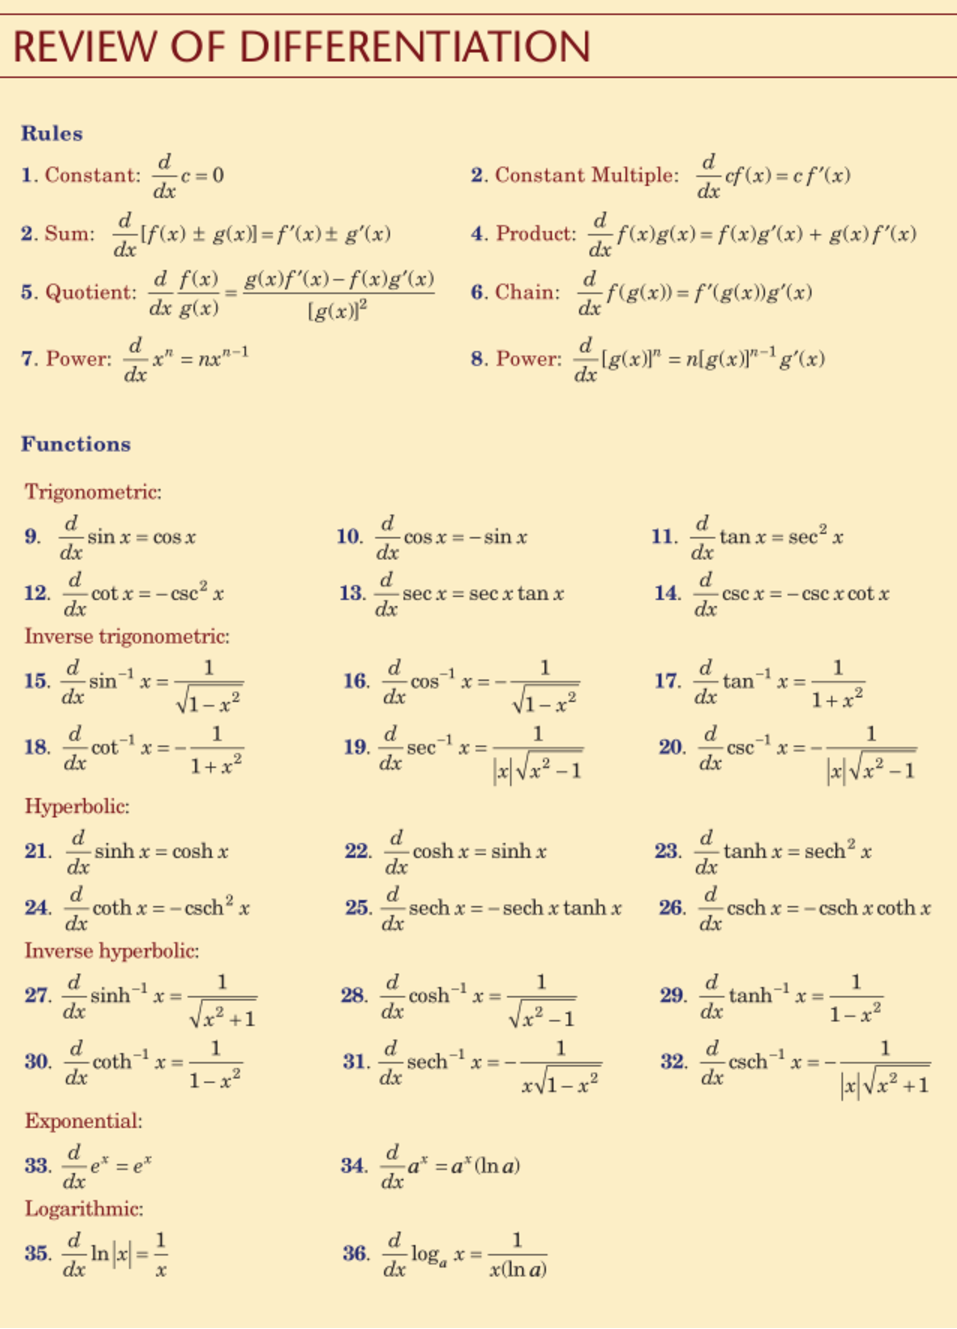
\includepdf[pages=1,pagecommand=\thispagestyle{fancy}, scale=0.8, pagecommand={\footnotetext{This "Review of Differentiation" is taken directly from Dennis G. Zill - A First Course in Differential Equations, 10th Ed. When time permits it will be re-created in an original format.}}]{Resources/DiffEQTable}
\newpage
\begin{fancybox}[Repeating product rule applied to arbitrary functions]{}
	Let $f:\mathbb{R}\rightarrow\mathbb{R}$ and $g:\mathbb{R}\rightarrow\mathbb{R}$ be continuous and differentiable functions of the variable $x$. Then the $m^{\textrm{th}}$ derivative of $f(x)g(x)$ with respect to $x$ is
	\begin{align*}
	\frac{d^m}{dx^m}f(x)g(x)=\sum_{i=0}^{n}{{n}\choose{i}}\bigg[\frac{d^i}{dx^i}f(x) \bigg]\bigg[\frac{d^{n-i}}{dx^{n-i}}g(x) \bigg].
	\end{align*}
\end{fancybox}




\section{Legendre differential equation}
The \textbf{Legendre polynomials}\index{Legendre polynomials} are normalized solutions to the Legendre differential equation
\begin{align}
	(1-x^2)\frac{d^2y}{dx^2}-2x\frac{dy}{dx}+\ell(\ell+1)y=0.
\end{align}
which have the general solution below. For even $\ell$, we must take $a_1 = 0$ to obtain a convergent solution, and for odd $\ell$, we must take $a_0 = 0$.
\begin{align}
	y=&a_0\left[1-\frac{\ell(\ell+1)}{2!}x^2+\frac{\ell(\ell+1)(\ell-2)(\ell+3)}{4!}x^4-\cdots\right] \\&+a_1\left[x-\frac{(\ell-1)(\ell+2)}{3!}x^3+\frac{(\ell-1)(\ell+2)(\ell-3)(\ell+4)}{5!}x^5-\cdots\right]
\end{align}
The Legendre polynomial $P_\ell(z)$ can be defined by the contour integral
\begin{align}
	P_\ell(z) = \frac{1}{2\pi i}\oint (1-2tz+t^2)^{-1/2}t^{-\ell-1} dt.
\end{align}
The first few Legendre Polynomials follow as:
\begin{multicols}{2}
	\noindent
\begin{align}
	P_0(x) &=1 \\
	P_1(x) &= x \\
	P_2(x) &= \frac{1}{2}(3x^2-1) \\
	P_3(x) &= \frac{1}{2}(5x^3 -3x) 
\end{align}
\begin{align}
	P_4(x) &= \frac{1}{8}(35x^4 - 30x^2 +3) \\
	P_5(x) &= \frac{1}{8}(63x^5-70x^3+15x) \\
	&\vdots \nonumber
\end{align}
\end{multicols}
The Rodrigues representation provides a formula for solving for the Legendre Polynomials
\begin{align}
	P_\ell(x) = \frac{1}{2^\ell \ell!}\frac{d^\ell}{dx^\ell}(x^2-1)^\ell
\end{align}
The Legendre polynomials are orthogonal over $(-1,1)$ with weighting function 1 and satisfy
\begin{align}
	\int_{-1}^{1}P_m(x)P_n(x)dx = \frac{2}{2n+1}\delta_{mn} \hspace{1cm} \textrm{and}\hspace{1cm}	\int_{0}^{1}P_m(x)P_n(x)dx = \frac{1}{2n+1}\delta_{mn}
\end{align} 
The associated Legendre differential equation is given by
\begin{align}
	\frac{d}{dx}\left[(1-x^2)\frac{dy}{dx}\right]
	+\left[\ell(\ell-1)-\frac{m^2}{1-x^2}\right]y=0
\end{align}
When $m,\ell \in \mathbb{Z}^+$ and $m \leq \ell$, the solutions to the above  equation are the \textbf{associated Legendre polynomials},
\begin{align}
	P_\ell^m(x) = (-1)^m(1-x^2)^{m/2}\frac{d^m}{dx^m}P_\ell(x) = \frac{(-1)^m}{2^\ell \ell!}(1-x^2)^{m/2}	\frac{d^{\ell+m}}{dx^{\ell+m}}(x^2-1)^\ell
\end{align}
The associated Legendre polynomials for $m < 0$ are defined by
\begin{align}
	P_\ell^{-m}(x) = (-1)^m \frac{(\ell - m)!}{(\ell+m)!}P_\ell^m(x)
\end{align}
The first few associated Legendre Polynomials with $m>0$ are
\begin{multicols}{2}
	\noindent
	\begin{align}
		P_0^0(x) &= 1 \\
		P_1^0(x) &= x \\
		P_1^1(x) &= -(1-x^2)^{1/2} \\
		P_2^0(x) &=\frac{1}{2}(3x^2-1) \\
		P_2^1(x) &= -3x(1-x^2)^{1/2} \\
		P_2^2(x) &= 3(1-x^2)
	\end{align}
	\begin{align}
		P_3^0(x) &= \frac{1}{2}x(5x^2-3) \\
		P_3^1(x) &= \frac{3}{2}(1-5x^2)(1-x^2)^{1/2} \\
		P_3^2(x) &= 15x(1-x^2) \\
		P_3^3(x) &= -15(1-x^2)^{3/2} \\
		&\vdots \nonumber
	\end{align}
\end{multicols}
The first few associated Legendre Polynomials with $m<0$ are
\begin{multicols}{2}
	\noindent
	\begin{align}
		P_1^{-1}(x) &= \frac{1}{2}(1-x^2)^{1/2} \\
		P_2^{-1}(x) &= \frac{1}{2}x(1-x^2)^{1/2} \\
		P_2^{-2}(x) &= \frac{1}{8}(1-x^2) \\
		P_3^{-1}(x) &= \frac{1}{8}(5x^2-1)(1-x^2)^{1/2} 
	\end{align}
	\begin{align}
		P_3^{-2}(x) &= \frac{1}{8}x(1-x^2) \\
		P_3^{-3}(x) &= \frac{1}{48}(1-x^2)^{3/2} \\
		P_4^{-1}(x) &= \frac{1}{8}(7x^3-3x)(1-x^2)^{1/2}\\
		&\vdots \nonumber
	\end{align}
\end{multicols}
The associated Legendre polynomials are orthogonal over $[-1,1]$ such that
\begin{align}
\int_{-1}^{1}P_\ell^m(x)P_{\ell'}^m(x)dx &= \frac{2}{2\ell+1}\frac{(\ell+1)!}{(\ell-1)!}\delta_{\ell\ell'} \\
\int_{-1}^{1}P_\ell^m(x)P_{\ell}^{m'}(x)\frac{dx}{1-x^2} &= \frac{(\ell+m)!}{m(\ell-m)!}\delta_{mm'}
\end{align}
The derivative about the origin for an associated Legendre polynomial is given by
\begin{align}
	\left[\frac{dP_\ell^m(x)}{dx}\right]_{x=0} = \frac{2^{m+1}\sin\left[\frac{1}{2}\pi(\ell+m)\right]\Gamma\left(\frac{1}{2}\ell+\frac{1}{2}m+1\right)}{\pi^{1/2
	}\Gamma\left(\frac{1}{2}\ell-\frac{1}{2}m+\frac{1}{2}\right)}
\end{align}
	


\newpage
\section{Laguerre differential equation}
The general associated Laguerre differential equation is defined by,
\begin{align}
	xy''(x)+(k+1-x)y'(x)+n y(x)=0.
\end{align}
A solution to the above differential equation is any generalized \textbf{Laguerre polynomial}\index{Laguerre polynomials} $L_n^k(x)$. The Rodrigues representation for the associated Laguerre polynomials is
\begin{align}
	L_n^k &= \frac{e^{x}x^{-k}}{n!}\frac{d^n}{dx^n}(e^{-x}x^{n+k}) 
	=(-1)^k\frac{d^k}{dx^k}[L_{n+k}(x)] = \sum_{m=0}^{n}\frac{(-1)^m(n+k)!x^m}{(n-m)!(k+m)!m!}.
\end{align} 
An alternate definitions of the Laguerre polynomials is given as
\begin{align}
	L_n^k(x)=\frac{1}{n!}\sum_{i=0}^{n}\frac{n!}{i!}{{k+n}\choose{n-i}}(-x)^i.
\end{align}
The associated Laguerre polynomials are orthogonal over $[0,\infty)$ in the following way,
\begin{align}
	\int_{0}^{\infty}e^{-x}x^kL_n^k(x)L_m^k(x)dx=\frac{(n+k)!}{n!}\delta_{mn}.
\end{align}
They also satisfy,
\begin{align}
	\int_{0}^{\infty}e^{-x}x^{k+1}[L_n^k(x)]^2dx=\frac{(n+k)!}{n!}(2n+k+1).
\end{align}
The first few Associated Laguerre polynomials are
\begin{align}
	L_0^k(x) &= 1 \\
	L_1^k(x) &= -x+k+1 \\
	L_2^k(x) &= \frac{1}{2}\left[x^2-2(k+2)x+(k+1)(k+2)\right]	\\
	L_3^k(x) &= \frac{1}{6}\left[-x^3+3(k+3)x^2-3(k+2)(k+3)x+(k+1)(k+2)(k+3)\right] \\
	&\vdots
\end{align}
A special case of the Associated Laguerre polynomials occurs when $k=0$ which can be defined by a sum, the Rodrigues representation, or the contour integral (respectively)
\begin{align}
	L_n(x) = \sum_{k=0}^{n}\frac{(-1)^k}{k!}{{n}\choose{k}}x^k \equiv \frac{e^x}{n!}\frac{d^n}{dx^n}(x^ne^{-x}) \equiv \frac{1}{2\pi i}\oint \frac{e^{-zt/(1-t)}}{(1-t)t^{n+1}}dt
\end{align}






\newpage
\section{Second-order Homogeneous}
\begin{align}
	\ddot{x}=0 &\implies x(t)=C_1x+C_2 \\
	\ddot{x}+Ax=0 &\implies x(t)=C_1e^{i\sqrt{A}t}+C_2e^{-i\sqrt{A}t} \\ &\implies x(t)=C_1\cos(\sqrt{A}t)+C_2\sin(\sqrt{A}t) \\
	\ddot{x}-Ax=0 &\implies x(t)=C_1e^{\sqrt{A}t}+C_2e^{-\sqrt{A}t} \\
	&\implies x(t)=C_1\sinh(\sqrt{A}t)+C_2\cosh(\sqrt{A}t) \\
	\ddot{x}\pm A \ddot{x}^2=0 &\implies x(t) = C_1\pm\frac{C_2}{A}\log(Ax\mp C_1) \\
	\ddot{x}\pm \frac{A}{x} \ddot{x}=0 &\implies x(t) = \frac{C_1}{1\mp A}x^{1\mp A}+C_2
\end{align} 



\begin{fancybox}[$\ddot{x}+A\dot{x}+Bx =0$]{}
Given any differential equation of the form $\ddot{x}+A\dot{x}+Bx =0$, a general solution of the following form exists:
\begin{align}
x(t)=C_1\exp\bigg[-\frac{1}{2}t(\sqrt{A^2-4B}+A)\bigg] +C_2\exp\bigg[\frac{1}{2}t(\sqrt{A^2-4B}-A)\bigg].
\end{align}
Following this, three special cases arise
\begin{enumerate}[(i)]
	\item $A^2>4B \implies$
	\begin{align}
	x(t)=C_1\exp\bigg[\frac{-At}{2}\bigg]\cosh\bigg(\frac{t\sqrt{A^2-4B}}{2} \bigg) +C_2\exp\bigg[\frac{-At}{2}\bigg]\sinh\bigg(\frac{t\sqrt{A^2-4B}}{2} \bigg)
	\end{align}
	\item $A^2<4B \implies$
	\begin{align}
	x(t)=C_1\exp\bigg[\frac{-At}{2}\bigg]\cos\bigg(\frac{t\sqrt{4B-A^2}}{2} \bigg) +C_2\exp\bigg[\frac{-At}{2}\bigg]i\sin\bigg(\frac{t\sqrt{4B-A^2}}{2} \bigg)	
	\end{align}
	\item $A^2=4B \implies $
	\begin{align}
	x(t)=C_1\exp\bigg[\frac{-At}{2}\bigg]
	\end{align}
\end{enumerate}
\end{fancybox}













\section{Second-order Linear Ordinary}
\begin{align}
\ddot{x}+Ax=B &\implies x(t)=\frac{B}{A}+C_1e^{i\sqrt{A}t}+C_2e^{-i\sqrt{A}t} \\ &\implies x(t)=\frac{B}{A}+C_1\cos(\sqrt{A}t)+C_2\sin(\sqrt{A}t) \\
\ddot{x}-Ax=B &\implies x(t)=-\frac{B}{A}+C_1e^{\sqrt{A}t}+C_2e^{-\sqrt{A}t} \\
&\implies x(t)=-\frac{B}{A}+C_1\sinh(\sqrt{A}t)+C_2\cosh(\sqrt{A}t) \\
\ddot{x}+x=t(A-t) &\implies x(t)=C_1\cos(t)+C_2\sin(t)-t^2+At+2 \\ 
\ddot{x}+A\dot{x}+Bx =t &\implies x(t)=C_1\exp\bigg[-\frac{1}{2}t(\sqrt{A^2-4B}+A)\bigg] \\& \hspace{3cm} +C_2\exp\bigg[\frac{1}{2}t(\sqrt{A^2-4B}-A)\bigg]-\frac{A}{B^2}+\frac{t}{B} \\
\ddot{x}+2\beta\dot{x}+\omega_0^2x=f_0e^{i\omega t} &\implies x(t)=\frac{f_0e^{i\omega t}}{\omega_0^2-\omega^2+2\beta i\omega} \\
&\implies x(t)=A\cos(\omega t-\delta)+A_{tr}e^{-\beta t}\cos(\omega_1t-\delta_{tr}) \\
&\hspace{1.6cm}\delta=\arctan\bigg(\frac{2\beta \omega}{\omega_0^2-\omega^2} \bigg) \\
&\implies x(t)=A\cos(\omega t-\delta)+e^{-\beta t}[B_1\cos(\omega_1 t)+B_2\sin(\omega_1 t)] \\
\ddot{x}+2\beta\dot{x}+x=te^{-\alpha t} &\implies x(t)=C_1e^{-\alpha t}+C_2te^{-\alpha t}+C_3e^{-\beta t}\sin(\omega_1 t)+C_4e^{-\beta t}\cos(\omega_1 t) \\
&\hspace{1.4cm}\omega_1^2=1-\beta^2
\end{align}




\section{Higher Order Differential Equations}
\begin{fancybox}[Particular solution to a sum of exponential functions]{}
	Let $f:\mathbb{R}\rightarrow\mathbb{R}$ be a continuous and differential function and let $C_n$, $a_n$, $b_n$ and $k_n$ be constant for all $n$. Given a differential equation of the form
	\begin{align*}
	\frac{d^n}{dt^n}f(t)+&\frac{d^{n-1}}{dt^{n-1}}C_{n-1}f(t)+\cdots+\frac{d}{dt}C_1f(t)+C_0f(t)=\sum_{i=0}^{\ell}a_i e^{k_i t},
	\end{align*}
	A solution of the following form exists:
	\begin{align*}
	f(t)=\sum_{i=0}^{\ell}b_i e^{k_i t}=\sum_{i=0}^{\ell}\frac{a_ie^{k_it}}{k_{\ell-i}^n +C_{n-1} k_{\ell-i}^{n-1} +\cdots+C_0} 
	\end{align*}
\end{fancybox}



\newpage
\section{Frobenius Method\index{Frobenius Method}}
Consider a second-order ordinary differential equation
\begin{align}
 	y''+P(x)y'+Q(x)y=0.
\end{align}
If P(x) and Q(x) remain finite at $x=x_0$, then $x_0$ is called an ordinary point. If either P(x) or Q(x) diverges as $x\rightarrow x_0$, then $x_0$ is called a singular point. If either P(x) or Q(x) diverges as $x\rightarrow x_0$ but $(x-x_0)P(x)$ and $(x-x_0)^2Q(x)$ remain finite as $x\rightarrow x_0$, then $x=x_0$ is called a \textbf{regular singular point} (or nonessential singularity)\cite{bib:Wolfram}. 
\begin{center}
	\noindent\makebox[\linewidth]{\rule{\textwidth}{0.4pt}}
\end{center}
If $x=0$ is a regular singular point of the ordinary differential equation, $y''(x)+P(x)y'(x)+Q(x)y(x)=0$, solutions may be found by the Frobenius method or by expansion in a Laurent series. In the Frobenius method, assume a solution of the form 
\begin{align}
	y(x) = x^\alpha \sum_{n=0}^{\infty}a_n x^n = \sum_{n=0}^{\infty}a_n x^{n+\alpha}.
\end{align}
Taking the first and second derivative of this with respect to $x$ yield
\begin{align}
	y'(x) &= \sum_{n=0}^{\infty}(n+\alpha)a_n x^{n+\alpha-1}, \hspace{1cm}\textrm{and}\hspace{1cm}
	y''(x) = \sum_{n=0}^{\infty}(n+\alpha)(n+\alpha-1)a_n x^{n+\alpha-2}.
\end{align}
If we allow $xP(x) = p_0+p_1x+p_2x^2+\cdots$ and $x^2Q(x) = q_0+q_1x+q_2x^2+\cdots$, then we can consolidate coefficients, take the limit as $x \rightarrow 0$ and arise at an \textbf{Indicial equation} to solve for possible $\alpha$ values
\begin{align}
	0&=\alpha(\alpha-1)+\alpha p_0+q_0 \hspace{0.5cm}\textrm{with} \hspace{0.5cm}\begin{cases}
	p_0 = \lim\limits_{x \rightarrow 0} xP(x) \\
	q_0 = \lim\limits_{x \rightarrow 0} x^2Q(x)
	\end{cases}
\end{align}
\begin{fancybox}[Fuchs's Theorem\index{Fuchs's Theorem} \cite{bib:Wolfram}]{1}
	At least one power series solution will be obtained when applying the Frobenius method if the expansion point is an ordinary, or regular, singular point. The number of roots is given by the roots of the indicial equation. 
\end{fancybox}
When the roots of the indicial equation are the same (or sometimes when they differ by an integer), there will be a Frobenious series solution $S_1(x)$ and another solution (where $S_2(x)$ is another Frobenious series) of the form
\begin{align}
	y(x) = S_1(x)\ln(x)+S_2(x) \implies y(x) = \ln(x)\sum_{n=0}^{\infty}a_n x^{n+\alpha} +\sum_{n=0}^{\infty}b_n x^{n+\beta}.
\end{align}



\newpage
\chapter{Integrals}
\thispagestyle{fancy}
Basic indefinite integrals ($c=$constant)
\begin{align}
	&\int \frac{dx}{a^2+x^2} = \frac{1}{a}\arctan\bigg(\frac{x}{a}\bigg) +c\\
	&\int \frac{dx}{\sqrt{a^2-x^2}}= \textrm{arcsin}\bigg(\frac{x}{|a|} \bigg)+c =\arctan\bigg(\frac{x}{\sqrt{a^2-x^2}} \bigg)+c\\
	&\int \frac{dx}{x+x^2} =\ln\bigg(\frac{x}{1+x} \bigg) +c\\
	&\int \frac{dx}{\sqrt{x^2-1}}= \textrm{arccosh}(x) +c\\
	&\int \frac{dx}{x\sqrt{x^2-1}}= \arccos\bigg(\frac{1}{x}\bigg)+c \\
	&\int \frac{dx}{(a^2+x^2)^{3/2}} = \frac{x}{a^2\sqrt{a^2+x^2}} +c\\
	&\int \frac{xdx}{(a^2+x^2)^{3/2}} = -\frac{1}{\sqrt{a^2+x^2}} +c\\
	&\int \frac{dx}{1-x^2} = \textrm{arctanh}(x) +c\\
	&\int \frac{dx}{\sqrt{a^2+x^2}} = \textrm{arcsinh}\bigg(\frac{x}{a}\bigg) +c = \ln\big|x+\sqrt{a^2+x^2}\big|+c\\
	&\int \frac{xdx}{1+x^2} =\frac{1}{2}\ln(1+x^2) +c\\
	&\int \frac{xdx}{\sqrt{1+x^2}}= \sqrt{1+x^2} +c\\
	&\int \frac{\sqrt{x}dx}{\sqrt{1-x}}= \arcsin(\sqrt{x})-\sqrt{x(1-x)} +c\\
	&\int \frac{x^2}{a^2+x^2} dx=\frac{-x}{2}\sqrt{a^2-x^2}+\frac{a^2}{2}\sin^{-1}\left(\frac{x}{a}\right)+c\\
	&\int \frac{1}{(a^2+x^2)^2}dx = \frac{x}{2a^2(x^2+a^2)}+\frac{1}{2a^3}\arctan\left(\frac{x}{a}\right) +c \\
	&\int \frac{x^2}{(a^2+x^2)^2}dx = \frac{-x}{2(x^2+a^2)}+\frac{1}{2a}\arctan\left(\frac{x}{a}\right) +c \\
	&\int \ln(x)=x\ln(x)-x+c 
\end{align}

\invisiblesection{Brief Table of Integrals}
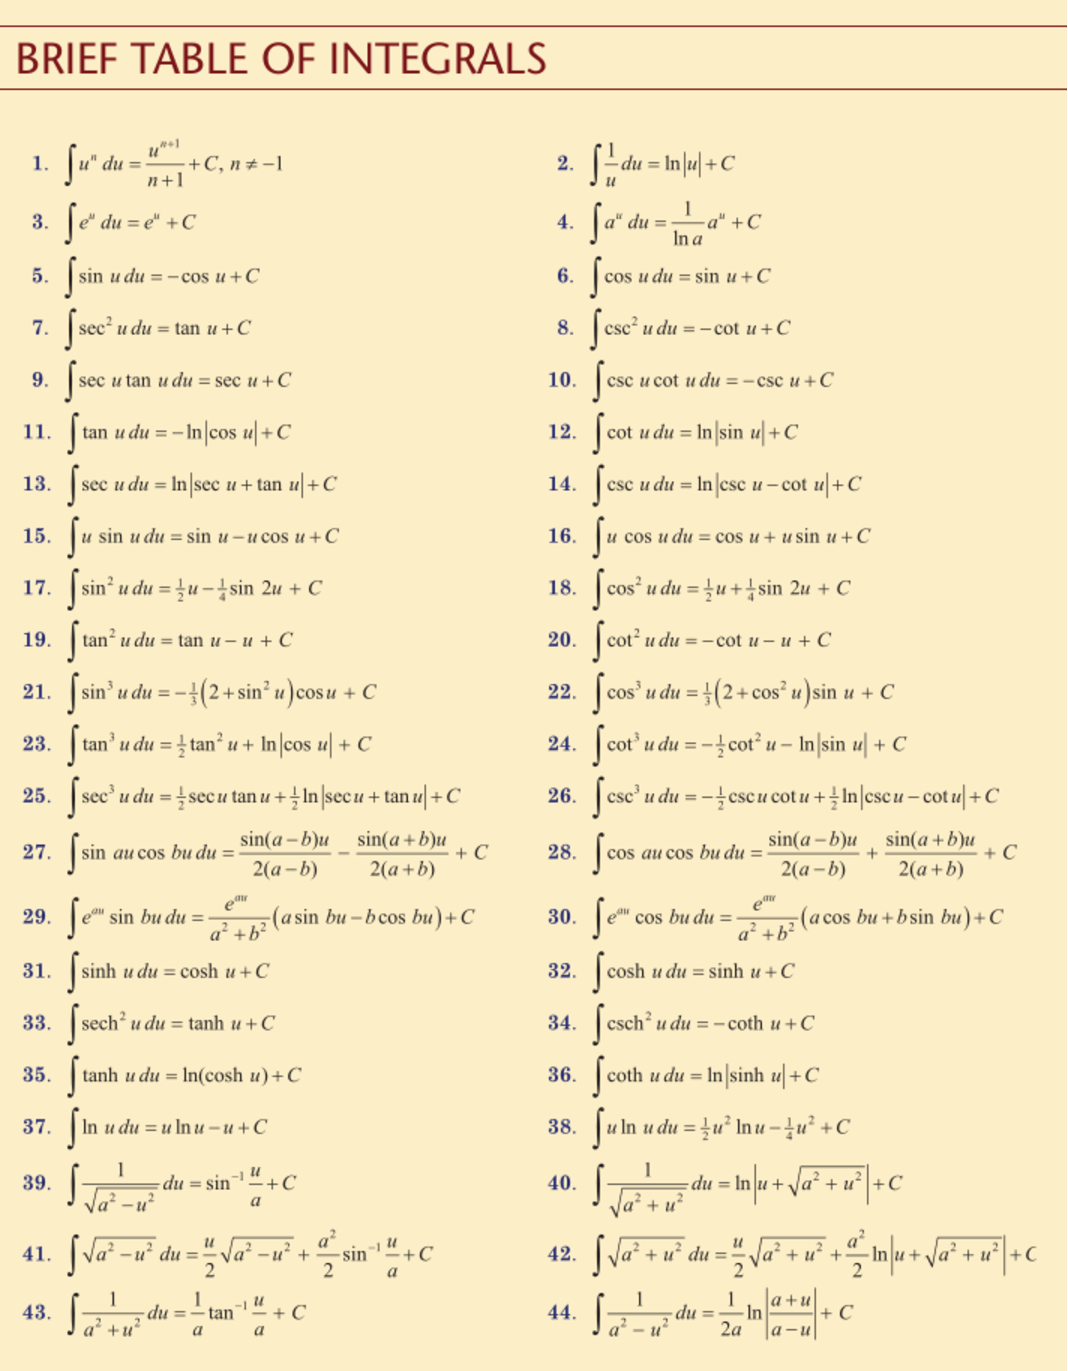
\includepdf[pages=1,pagecommand=\thispagestyle{fancy}, scale=0.8, pagecommand={\footnotetext{This "Brief Table of Integrals" is taken directly from Dennis G. Zill - A First Course in Differential Equations, 10th Ed. When time permits it will be re-created in an original format.}}]{Resources/IntegralTable}
\newpage

Exponential integrals
\begin{align}
	&\int_{-\infty}^{\infty} \frac{e^{-iax}}{(1+x^2)}dx = \pi e^{-|a|}
\end{align}
Trigonometric integrals 
\begin{align}
	&\int \tan(x)dx = -\ln(\cos(x)) +c\\
	&\int \tanh(x)dx = \ln(\cosh(x))+c \\
	&\int \sin^2(x)dx = \frac{1}{2}\big(x-\sin(x)\cos(x)\big)+c = \frac{1}{4}\big(2x-\sin(2x)\big)+c\\
	&\int \cos^2(x)dx = \frac{1}{2}\big(x+\sin(x)\cos(x)\big)+c = \frac{1}{4}\big(2x+\sin(2x)\big)+c \\
	&\int \sin^2(x)\cos(x)dx = \frac{1}{3}\sin^3(x)+c \\
	&\int \cos^2(x)\sin(x)dx = -\frac{1}{3}\cos^3(x)+c \\
	&\int \sin^3(x)dx = -\frac{1}{3}\cos(x)\big(\sin^2(x)+2\big)+c \\
	&\int x\sin^2(x)dx = \frac{1}{4}\big(x^2-x\sin(2x)-\frac{1}{2}\cos(2x)\big)+c\\
	&\int x^2\sin^2(x)dx =\frac{x^3}{6}-\bigg(\frac{x^2}{4}-\frac{1}{8}\bigg)\sin(2x)-\frac{x}{4}\cos(2x)+c \\
	&\int x^n \sin(ax)dx = -\frac{x^n}{a}\cos(ax)+ \frac{n}{a}\int x^{n-1}\cos(ax)dx \\
	&\int x^n \cos(ax)dx = \frac{x^n}{a}\sin(ax)- \frac{n}{a}\int x^{n-1}\sin(ax)dx		
\end{align}
The Wallis Cosine Formula
\begin{align}
\int_{0}^{\pi/2}\cos^n(x) dx = \int_{0}^{\pi/2}\sin^n(x) dx = \frac{(n-1)!!}{n!!}
\begin{cases}
\pi/2 &\textrm{ for } n=2,4,\dots\\
1 &\textrm{ for } n=3,5,\dots\\
\end{cases}
\end{align}




\newpage
\section{Gaussian Integrals}
The integral of an arbitrary Gaussian function is
\begin{align}
\int x^ne^{\beta x} dx = e^{\beta x}\sum_{k=0}^{n}(-1)^k\frac{n!x^{n-k}}{(n-k)!\beta^{k+1}}+c
\end{align}
Some general Gaussian integrals evaluate as
\begin{align}
\int_{-\infty}^{\infty} e^{-\alpha x^2} dx = \sqrt{\frac{\pi}{\alpha}} 
\end{align}
\begin{multicols}{2}
	\noindent
\begin{align}
I_n&=\int x^ne^{-x/\alpha}dx \\
I_0&= -\alpha e^{-x/\alpha} \\
I_1&= -(\alpha^2+\alpha x) e^{-x/\alpha} \\
I_2&= -(2\alpha^3+2\alpha^2 x+\alpha x^2) e^{-x/\alpha} \\
I_{n+1}&=\alpha^2\frac{\partial  I_n}{\partial \alpha} 
\end{align}
\begin{align}
&\int_{0}^{\infty}e^{-x/\alpha}dx = \alpha \\
&\int_{0}^{\infty}xe^{-x/\alpha}dx = \alpha^2 \\
&\int_{0}^{\infty}x^2e^{-x/\alpha}dx = 2\alpha^3 \\
&\int_{0}^{\infty}x^ne^{-x/\alpha}dx = n!\alpha^{n+1}
\end{align}
\end{multicols}
The integral of an arbitrary Gaussian function with an n-dimensional linear term (with $n \in \mathbb{Z}$) is
\begin{align}
\int_{0}^{\infty}x^{2n}e^{-\alpha x^2}dx = \sqrt{\frac{\pi}{\alpha}}\frac{(2n-1)!!}{2^{n+1}\alpha^n} &\implies  \int_{-\infty}^{\infty}x^{2n}e^{-\alpha x^2}dx = \sqrt{\frac{\pi}{\alpha}}\frac{(2n-1)!!}{(2\alpha)^n}\\
\int_{0}^{\infty}x^{2n+1}e^{-\alpha x^2}dx = \frac{n!}{2a^{n+1}} &\implies \int_{-\infty}^{\infty}x^{2n+1}e^{-\alpha x^2}dx = 0
\end{align}
Therefore a general solution is
\begin{align}
\int_{0}^{\infty}x^ne^{-\alpha x^2}dx = 
\begin{cases}
\displaystyle
\frac{(n-1)!!}{2^{n/2+1}a^{n/2}}\sqrt{\frac{\pi}{\alpha}} & \textrm{ for $n$ even} \\
\displaystyle
\frac{[\frac{1}{2}(n-1)]!}{2a^{(n+1)/2}}& \textrm{ for $n$ odd} 
\end{cases}
\end{align}
The below form of a gaussian integral evaluates to zero when $n$ is odd due to the function being odd, but when $n$ is even, the more general integral has the following closed form
\begin{align}
\int_{-\infty}^{\infty} x^ne^{-\alpha x^2+\beta x}=\sqrt{\frac{\pi}{\alpha}}e^{\beta^2/(4\alpha)}\sum_{k=0}^{\lfloor n/2\rfloor} {{n}\choose{2k}} (2k-1)!!(2a)^{k-n}\beta^{n-2k}
\end{align}


\newpage
\chapter{Fourier Series} \index{Fourier Series}
\thispagestyle{fancy}
The computation of the (usual) Fourier series is based on the integral identities 
\begin{multicols}{2}\noindent
\begin{align}
&\int_{-\pi}^{\pi}\sin(mx)\sin(nx)dx=\pi\delta_{mn} \\
&\int_{-\pi}^{\pi}\cos(mx)\cos(nx)dx=\pi\delta_{mn} \\
&\int_{-\pi}^{\pi}\sin(mx)\cos(nx)dx=0 
\end{align}
\begin{align}
&\int_{-\pi}^{\pi}\sin(mx)dx=0 \\
&\int_{-\pi}^{\pi}\cos(mx)dx=0 \\
&\delta_{mn} = \frac{1}{2\pi i}\oint_\gamma z^{m-n-1}dz
\end{align}
\end{multicols}
Using the method for a generalized Fourier series, the usual Fourier series involving sines and cosines is obtained by taking $f_1(x)=cosx$ and $f_2(x)=sinx$. Since these functions form a complete orthogonal system over $[-\pi,\pi]$, the Fourier series of a function $f(x)$ is given by (with $n\in \mathbb{N}$)
\begin{align}
f(x)&=\frac{1}{2}a_0+\sum_{n=1}^{\infty}a_n\cos(nx)+\sum_{n=1}^{\infty}b_n\sin(nx) \\
a_0&= \frac{1}{\pi} \int_{-\pi}^{\pi}f(x)dx \\
a_n&= \frac{1}{\pi} \int_{-\pi}^{\pi}f(x)\cos(nx)dx \\
b_n&= \frac{1}{\pi} \int_{-\pi}^{\pi}f(x)\sin(nx)dx
\end{align}
The notion of a Fourier series can also be extended to complex coefficients. 
\begin{align}
	f(x) &= \sum_{n=-\infty}^{\infty} A_n e^{inx} \hspace{0.5cm}\textrm{with}\hspace{0.5cm}
	A_n = \frac{1}{2\pi} \int_{-\pi}^{\pi}f(x)e^{-inx}dx
\end{align}
For a function f(x) periodic on an interval [-L,L] instead of [-pi,pi], a simple change of variables can be used to transform the interval of integration from [-pi,pi] to [-L,L]. Let 
\begin{align}
x &\equiv \frac{\pi x'}{L}  \Longleftrightarrow x'\equiv\frac{Lx}{\pi} \implies
dx = \frac{\pi dx'}{L}
\end{align}


\newpage
\chapter{Astronomy, Optics and Telescopes}
\thispagestyle{fancy}
\begin{multicols}{2}
A \textbf{parsec}\index{Parsec} is defined so
\begin{align}
1 \textrm{ parsec}=\frac{1\textrm{ AU}}{\tan(1")} \approx \frac{1\textrm{ AU}}{1"}
\end{align}
The \textbf{flux}\index{Flux} ($F$) of a star relates to it's luminosity ($L$) and distance ($d$) via
\begin{align}
F  &= \frac{L}{4\pi R^2} = \sigma_{SB} T_{eff}^4
\end{align}
The flux received by a telescope at distance d is then
\begin{align}
	F(d)  &= \frac{L}{4\pi d^2} = \sigma T_{eff}^4\left(\frac{R}{d}\right)^2
\end{align}
The ratio of two magnitudes using different filters from a single star gives a rough estimation of the stars color.
\begin{align}
B-V&=m_B-m_V=-2.5\log_{10}\bigg(\frac{F_B}{F_V}\bigg) \\
\frac{F_B}{F_V}&=10^{-(M_B-M_V)/2.5}
\end{align}
We define the \textbf{distance modulus}\index{Distance modulus} ($DM$) as the difference in apparent magnitude ($m$) between a given star and the absolute magnitude ($M$) it would have if it were at 10 pc.
\begin{align}
DM &\equiv m-m(10 \textrm{ pc}) \equiv m-M \\
M &\equiv m-DM
\end{align}
The full form of intensity as a function of angle from the beam axis is
\begin{align}
I=I_0\bigg[\frac{\sin(\pi D/\lambda \sin(\theta))}{\sin(\pi d/\lambda \sin(\theta))} \bigg]^2
\end{align}
Snell's Law: 
\begin{align}
\frac{\sin(\theta_1)}{\sin(\theta_2)} = \frac{v_1}{v_2} = \frac{\lambda_1}{\lambda_2}=\frac{n_2}{n_1}
\end{align}






\section{Celestial Orbits}
Suppose we have a exoplanet system with a planet $p$ and a star $s$. The vector from the star to the planet is $\vec{r}_{sp}=\vec{r}_p-\vec{r}_s$, and the force that the star exerts on the planet is ($\vec{r}_n$ is the vector from the origin to $n$)
\begin{align}
\vec{F}_{sp}=-\frac{GM_pM_s}{|\vec{r}_{sp}|^3}\vec{r}_{sp}
\end{align}
If we put the origin at the center of mass ($\vec{R}$ is the vector from the origin to the center of mass)
\begin{align}
\vec{R}=\frac{M_s\vec{r}_s+M_p\vec{r}_p}{M_s+M_p}
\end{align}
Then the star and planets have positions
\begin{align}
\vec{x}_s &= \vec{r}_s-\vec{R}=-\frac{M_p}{M_p+M_s}\vec{r}_{sp} \\
\vec{x}_p &= \vec{r}_p-\vec{R}=-\frac{M_s}{M_p+M_s}\vec{r}_{sp} 
\end{align}
And thus accelerations
\begin{align}
\frac{d^2\vec{x}_s}{dt^2} &=-\frac{M_p}{M_p+M_s}\frac{d^2 \vec{r}_{sp}}{dt^2} \\
\frac{d^2\vec{x}_p}{dt^2} &=-\frac{M_s}{M_p+M_s}\frac{d^2 \vec{r}_{sp}}{dt^2} 
\end{align}
Substituting the acceleration into the equation of motion for the planet,
\begin{align}
M_p\frac{d^2 \vec{x}_p}{dt^2}=\vec{F}_{sp}
\end{align}
Then we can get the reduced equation of motion as
\begin{align}
\frac{d^2 \vec{r}_{sp}}{dt^2}=-G\frac{M_s+M_p}{|\vec{r}_{sp}|^3}\vec{r}_{sp}
\end{align}
Keplar's Third law: The solution to this is an elliptical orbit with the center-of-force at one focus of the ellipse. The period ($T$) depends on the semi-major axis ($a$)
\begin{align}
T^2=\frac{4\pi^2}{G(M_s+M_p)}a^3 \\
a^3=\frac{G(M_s+M_p)}{4\pi^2}T^2
\end{align}
If the orbit is circular, so that $|\vec{r}_sp=a$ is constant, then the orbital speed of the star is
\begin{align}
v_s=\frac{2\pi aM_p}{T(M_p+M_s)}=\sqrt{\frac{GM_p^2}{a(M_p+M_s)}}
\end{align}
For a particle in a circular orbit, $v = r\Omega \hat{\theta}$; using Kepler’s law (r is the distance from the center of mass), we have
\begin{align}
L=mr^2\Omega = m\sqrt{GMr}.
\end{align}
The orbital angular momentum of the two-body system is
\begin{align}
L&=\frac{M_1M_2}{M_1+M_2} a^2\Omega\\
&= \frac{M_1M_2}{M_1+M_2}\sqrt{G(M_1+M_2)a}.
\end{align}
The angular momentum of a sphere is
\begin{align}
L=\frac{8\pi}{15}\rho\Omega R^5=\frac{2}{5}MR^2\Omega.
\end{align}
The equations of motion in a rotating frame are
\begin{align}
\frac{d^2\vec{r}'}{dt^2}&=\frac{1}{m}\vec{F}_{rot} \\
&=\frac{1}{m}\vec{F}+\underbrace{r\Omega^2\hat{r}}_\text{centrifugal}+\underbrace{2\Omega(v_\theta\hat{r}-v_r\hat{\theta})}_\text{coriolis}.
\end{align}
Particles within a sphere of radius $R_H$ are dominated by the gravitational attraction of $M_2$; $R_H$ (the Hill radius) is
\begin{align}
R_H\approx a\bigg[\frac{M_2}{3(M_1+M_2)} \bigg]^{1/3}.
\end{align}





\section{Celestial \& Stellar Atmospheres}
The equation of hydrostatic equilibrium\index{Hydrostatic equilibrium}
\begin{align}
\frac{dP}{dr}=-\rho g.
\end{align}
The ideal gas law can be written (with $m$=mass of 1 mole of our gas) as 
\begin{align}
P=\bigg(\frac{mN/N_A}{V} \bigg)\frac{kN_A}{m}T\equiv \rho \frac{kN_A}{m}T.
\end{align}
Combining the above two equations and assuming $T$=constant then yields a relation between pressure and height as
\begin{align}
\frac{dP}{P}=-\frac{mg}{N_AkT}dz.
\end{align}
This then gives a pressure Dependant on height as
\begin{align}
P(z)=P_0\exp\bigg[-\frac{mgz}{N_AkT} \bigg].
\end{align}

In addition to the Coriolis acceleration from the Earth rotation, horizontal pressure gradients will also produce an acceleration
\begin{align}
-\frac{1}{\rho}\nabla P.
\end{align}
The equation for force and acceleration along r$\hat{r}$ is therefore
\begin{align}
\underbrace{\frac{v^2}{r}}_\text{centripital}+\underbrace{2v\Omega \sin(\lambda)}_\text{coriolis}-\underbrace{\frac{1}{\rho}\frac{dP}{dr}}_\text{pressure}=0.	
\end{align}
If matter is in thermal equilibrium, then populations of a two different
states of a given atom are given by Boltzmann’s formula\index{Boltzmann’s formula},
\begin{align}
	\frac{n_i}{n_j}=\frac{g_i}{g_j}exp\left(\frac{E_j-E_i}{kT}\right).
\end{align}
Hydrostatic equilibrium (where $m$ is the mass within a sphere of radius $r$, $P$ is the pressure, and $\rho$ is the mass density) gives two equations of stellar structure,
\begin{align}
	\frac{dm}{dr} &= 4\pi r^2 \rho \andspace{0.5cm}
	\frac{dP}{dr} = -\rho \frac{Gm}{r^2}
\end{align}
From the virial theorem, the average pressure and density are
\begin{align}
	\bar{\rho} &= \frac{GM}{4\pi R^3} \andspace{0.5cm}
	\bar{P} \propto \frac{GM^2}{R^4}
\end{align}
The optical depth for an outward-directed ray is
\begin{align}
	\tau_\mu = \int_z^\infty\rho \kappa_\mu dz' \implies \frac{d\tau}{dz}=-\rho \kappa
\end{align}
From this, an estimate of the photospheric pressure can be determined  for a gray atmosphere in LTE\footnote{Local Thermodynamical Equilibrium} by,
\begin{align}
	\frac{dP}{d\tau} = -\left(\frac{d\tau}{dz}\right)^{-1}\rho g = \frac{g}{\kappa}.
\end{align}
From hydrostatic equilibrium and taking $\rho=constant$ (where $\mu m_u$ is the average mass of a particle in the plasma), the central pressure and temperature are given by
\begin{align}
	T_c &=\frac{GM\mu m_u}{2Rk_B} \\
	P_c &= \frac{3GM^2}{8\pi R^4}
\end{align}
Bringing a small amount of mass $dm$ from infinity onto a sphere of mass m and radius r gives a potential change of
\begin{align}
	d\Omega = -\frac{Gm}{r}dm.
\end{align}
For a constant density, we have $r=R(m/M)^{1/3}$ and so
\begin{align}
	\Omega = -\frac{3GM^2}{5R}.
\end{align}
Using this, the mean temperature and pressure for a constant density sphere is
\begin{align}
	\bar{T} &= \frac{GM\mu m_u}{5Rk_B} \\
	\bar{P} &= \frac{3GM^2}{20\pi R^4}.
\end{align}
The free fall time it would take for a star to collapse if all internal pressures were removed is \begin{align}
	\tau_{ff} = \frac{\pi}{\sqrt{GM}}\left(\frac{R}{2}\right)^{3/2} = \left(\frac{3}{32\pi}\right)^{1/2}\frac{1}{\sqrt{G\bar{\rho}}}.
\end{align}
The \textbf{dynamical timescale}\index{Dynamical timescale} of the star is defined from the proportionality constant of the free fall time
\begin{align}
	t_{dyn} \equiv \frac{1}{\sqrt{G\bar{\rho}}}.
\end{align}
Any change in pressure is communicated through a star by sound waves which travel at the speed
\begin{align}
	c_s = \left(\gamma \frac{P}{\rho}\right)^{1/2}=\left(\gamma \frac{k_BT}{\mu m_u}\right)^{1/2}.
\end{align}
The time it takes for a sound wave to travel a distance R is then
\begin{align}
	\tau_{sc} = \frac{R}{c_s} = \sqrt{\frac{3R^3}{GM}} = \left(\frac{3}{2\sqrt{\pi}}\right)\frac{1}{\sqrt{G\bar{\rho}}}.
\end{align}
The \textbf{Kelvin-Helmholtz timescale} is the time it would take the sun to radiate all of it's gravitational energy away with it's current luminosity $L_\odot$,
\begin{align}
	t_{KH} \approx \frac{GM_\odot^2}{R_\odot L_\odot} \approx 3 \times 10^7 yr.
\end{align}
{\centering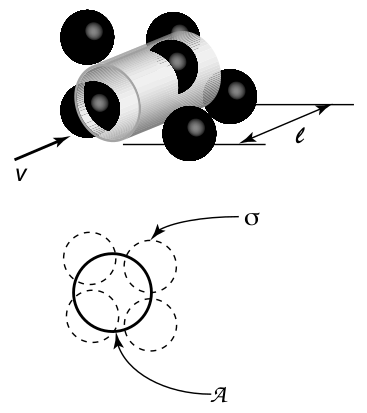
\includegraphics[width=0.8\columnwidth]{./Images/Diagrams/meanfreepath.png}}\\
As displayed by the image above\footnote{"Schematic of a particle incident on a group of particles." \cite{bib:AST304}.}, the probability of a particle making it through a density of obstacles $n$ with cross section $\sigma$ is
\begin{align}
	\mathcal{P} = \frac{n(\mathcal{A}\ell)\sigma}{\mathcal{A}} = n\sigma \ell.
\end{align}
The \textbf{mean free path} is defined to be the length at which $\mathcal{P}\rightarrow 1$ which is when the particle will suffer a collision:
\begin{align}
\ell = \frac{1}{n\sigma}.
\end{align}


\section{Convection}
The temperature gradient in a star ($\kappa= opacity$) is
\begin{align}
\frac{dT}{dr} = -\frac{3\rho\kappa}{4acT^3}\frac{L(r)}{4\pi r^2}.
\end{align}
From the first law of thermodynamics,
\begin{align}
dQ &= dU - \frac{P}{\rho^2}d\rho \\
dU &=  \left(\frac{\partial U}{\partial T}\right)_\rho dT +\left(\frac{\partial U}{\partial \rho}\right)_T d\rho \\
dQ &= \left(\frac{\partial U}{\partial T}\right)_\rho dT +\left[\left(\frac{\partial U}{\partial \rho}\right)_T- \frac{P}{\rho^2}\right] d\rho.
\end{align}
While holding density fixed, the heat needed to raise the temperature of one kilogram of fluid is then
\begin{align}
C_\rho \equiv \left(\frac{\partial Q}{\partial T}\right)_\rho = \left(\frac{\partial U}{\partial T}\right)_\rho.
\end{align}
From this, heat transfer can be expressed as a function of temperature and pressure
\begin{align}
dQ &= \left[C_\rho+\frac{P}{\rho T}\right]dT - \frac{1}{\rho}dP \\
&= \left[C_\rho+\frac{k_B}{\mu m_u}\right]dT - \frac{1}{\rho}dP.
\end{align}
Hence, while holding pressure fixed, the heat needed to raise the temperature of one kilogram of fluid is
\begin{align}
C_P = \left(\frac{\partial Q}{\partial T}\right)_P = C_\rho + \frac{k_B}{\mu m_u}.
\end{align}
For a plasma of ions and electrons,
\begin{align}
C_\rho =\frac{3k_B}{2\mu m_u} = \frac{3}{5} C_P.
\end{align}
Thus the ratio of specific heats for an ideal gas is
\begin{align}
\gamma = \frac{C_P}{C_\rho} = \frac{5}{3}.
\end{align}
During adiabatic motion, no heat exchange occurs and so $TdS = dQ =0$ which leads to
\begin{align}
T=T_0\left(\frac{P}{P_0}\right)^{(\gamma -1)/\gamma}.
\end{align}
The temperature change with pressure in an adiabatically stratified gas is given by
\begin{align}
\frac{P}{T}\left(\frac{\partial T}{\partial P}\right)_S = \left(\frac{\partial \ln T}{\partial \ln P}\right)_S = \frac{\gamma -1}{\gamma}.
\end{align}
For stable convection, we must have
\begin{align}
\left(\frac{\partial V}{\partial S}\right)_P\frac{dS}{dr} = \frac{T}{C_P}\left(\frac{\partial V}{\partial T}\right)_P\frac{dS}{dr} > 0.
\end{align}
The stability requirements for convection can also be derived in terms of local gradients of temperature and pressure. The fluid is unstable to convection if
\begin{align}
\frac{P}{P_{rad}}\frac{\kappa}{16\pi Gc}\frac{L(r)}{m(r)} > \left(\frac{\partial \ln T}{\partial \ln P}\right)_S = \frac{\gamma-1}{\gamma}.
\end{align}
\section{Main Sequence Stars}
For an enclosed mass we have the following relations for radiative and convective regions respectively
\begin{align}
	\frac{dT}{dr} &= -\frac{L}{4\pi r^2}\frac{3\rho \kappa}{4acT^3} \\
	\frac{dT}{dr} &= \frac{T}{P}\left(\frac{\partial \ln T}{\partial \ln P}\right)_S \frac{dP}{dr}.
\end{align}
The fourth order equation of stellar structure  (with $\epsilon$ being the heating rate per unit mass) is
\begin{align}
	\frac{dL}{dr} = 4\pi r^2\rho \epsilon.
\end{align}
\end{multicols}


\newpage
\chapter{Classical Mechanics}
\thispagestyle{fancy}
\begin{multicols}{2}
Newtons Second Law in Cartesian coordinates and 2D Polar coordinates
\begin{align}
\vec{F}=m\vec{a} = m\boldsymbol{{\ddot{r}}} &\Longleftrightarrow \begin{cases}
F_x = m\ddot{x} \\ F_y = m\ddot{y} \\ F_z = m\ddot{z}
\end{cases}
\\&\Longleftrightarrow \begin{cases}
F_r=m(\ddot{r}-r\dot{\phi}^2) \\
F_\phi=m(r\ddot{\phi}+2\dot{r}\dot{\phi})
\end{cases}
\end{align}
Conservation of energy
\begin{align}
E =\textrm{constant} &=KE+PE \\ &=\frac{1}{2}m|\vec{v}|^2+mgh
\end{align}
Equation of motion for a rocket
\begin{align}
m\dot{v}=-\dot{m}v_{ex}+F^{external}
\end{align}
The center of mass of several particles with a total mass $M$ is
\begin{align}
\vec{R} &=\frac{1}{M}\sum_{\alpha=1}^{n}m_\alpha\vec{r}_\alpha = \frac{m_1\vec{r}_1+\cdots m_n\vec{r}_n}{M} \\
\vec{R} &= \frac{1}{M}\int \vec{r} dm = \frac{1}{M} \int \rho \vec{r} dV 
\end{align}
The mass of an object is defined by the density multiplied by the volume.
\begin{align}
M\equiv \rho V\equiv \iiint_Q\rho(x,y,z) dV
\end{align}
The moment of inertia with respect to a given axis of a solid body with density $\rho(r)$, where $r_\perp$ is the perpendicular distance from the axis of rotation, is defined by the volume integral
\begin{align}
I \equiv \int \rho(\boldsymbol{r}) r_\perp^2 dV \equiv \iiint_{Q}\rho(x,y,z)||\boldsymbol{r}||^2dV 
\end{align}
Angular momentum
\begin{align}
\vec{L}=\vec{r}\times \vec{p}=I\vec{\omega}=I\dot{\theta}
\end{align}
The net external torque is given by
\begin{align}
\vec{\tau}_{ext} = \vec{r} \times \vec{F}= \frac{d\vec{L}}{dt}
\end{align}
The change in kinetic energy as it moves from point a to point b is
\begin{align}
\Delta K &\equiv K_2-K_1= \int_{a}^{b}\vec{F}\cdot d\vec{r} \equiv W(a \rightarrow b) \\
K &=\frac{1}{2}mv^2=\frac{1}{2}I\omega^2=\frac{1}{2}I\dot{\theta}^2
\end{align}
A force $\vec{F}$ on a particle is \textbf{conservative} if (i) it depends only on the particles position, $\vec{F}= \vec{F}(\vec{r})$ and (ii) $\nabla \times \vec{F} = 0$. If $\vec{F}$ is conservative we can define a corresponding \textbf{potential energy} so that
\begin{align}
U(\boldsymbol{r}) &= -W(\boldsymbol{r}_0 \rightarrow \boldsymbol{r}) \equiv \int_{\boldsymbol{r}_0}^{\boldsymbol{r}}\boldsymbol{F}(\boldsymbol{r} ')\cdot d\boldsymbol{r}' \\ 
\vec{F}&=-\nabla \vec{U}
\end{align}
Hooke's Law states that the force needed to extend or compress a spring by some distance is proportional to that distance.
\begin{align}
F=-kx \Longleftrightarrow U=\textrm{constant}+\frac{1}{2}kx^2
\end{align}	
Simple harmonic motion
\begin{align}
\ddot{x}=-\omega^2x \Longleftrightarrow A\cos(\omega t - \delta)
\end{align}
Damped oscillations: If the oscillator is subject to a damping force $-bv$, the
\begin{align}
\ddot{x}+2\beta\dot{x}+\omega_0^2x=0 \textrm{ and } \beta < \omega_0  \nonumber\\ \Longleftrightarrow x(t) =Ae^{-\beta t}\cos(\omega_1t-\delta) \\
\beta = \frac{b}{2m}, \textrm{ }\textrm{ }\textrm{ }
\omega_0 = \sqrt{\frac{k}{m}},\textrm{ }\textrm{ }\textrm{ }
\omega_1 = \sqrt{\omega_0^2-\beta^2}
\end{align}
If the oscillator is also subject to a sinusoidal driving force $F(t)=mf_0\cos(\omega t)$, the long-term motion has the form
\begin{align}
x(t)&=A\cos(\omega t-\delta) \\
A^2 &= \frac{f_0^2}{(\omega_0^2-\omega^2)^2+4\beta^2\omega^2}
\end{align}
\end{multicols}
It is always possible to write a sum of sinusoidal functions as a single sinusoid the form
\begin{align}
f(\theta)=A\cos(\theta)+B\sin(\theta) &\Longleftrightarrow  f(\theta)=C\cos(\theta+\delta) \\
\delta = \arctan(-B/A) \hspace{1cm}&\textrm{and}\hspace{1cm} C = \pm\sqrt{A^2+B^2} \\
f(\theta)=A\cos(\theta)+B\sin(\theta) &\Longleftrightarrow f(\theta)=\textrm{sgn}(A)\sqrt{A^2+B^2}\cos\big(\theta+\arctan(-B/A)\big)
\end{align} 


\begin{multicols}{2}
Any periodic function with period $\tau$ can be written as (A Fourier series with $n \geq 1$)
\begin{align}
f(t)&=\sum_{n=0}^{\infty}[a_n\cos(n\omega t)+b_n\sin(n\omega t)] \\
a_n&= \frac{2}{\tau}\int_{-\tau/2}^{\tau/2}f(t)\cos(n\omega t)dt \\
b_n&= \frac{2}{\tau}\int_{-\tau/2}^{\tau/2}f(t)\sin(n\omega t)dt \\
a_0&= \frac{1}{\tau}\int_{-\tau/2}^{\tau/2}f(t)dt
\end{align}
It is sometimes useful to express the above Fourier series as an exponential
\begin{align}
f(t)&=\sum_{n=-\infty}^{\infty}A_ne^{in\omega t} \\
A_n&=\frac{1}{\tau}\int_{-\tau/2}^{\tau/2}f(t)e^{-in\omega t}dt
\end{align} 
It is important to know $A_n=A^*_{-n}$ so we can write $A_n=\mathfrak{R}(A_n)+i\mathfrak{I}(A_n)$. An important relationship between $A_n$, $a_n$ and $b_n$ then follows as, 
\begin{align}
a_n&=2\mathfrak{R}(A_n)\hspace{0.3cm}\textrm{ and }\hspace{0.3cm} b_n=-2\mathfrak{I}(A_n)
\end{align}
The root-mean square displacement is a good measure of the average response of the oscillator and is given by parseval's theorem
\begin{align}
x_{rms}&=\sqrt{\frac{1}{\tau}\int_{0}^{\tau}x^2dt} \\ &=
\sqrt{A_0^2+\frac{1}{2}\sum_{n=1}^{\infty}A_n^2}
\end{align}
The non-relativistic Lagrangian $\mathcal{L}$ for a conservative system can be defined in terms of the kinetic energy and potential energy of a system as
\begin{align}
\mathcal{L}=KE-PE
\end{align}
An integral of the form
\begin{align}
S=\int_{x_1}^{x_2}f[y(x),y'(x),x]dx
\end{align}
taken along a path $y=y(x)$ is stationary with respect to variations of that path if and only if $y(x)$ satisfies the Euler-Lagrange Equation
\begin{align}
\frac{\partial f}{\partial y}-\frac{d}{dx}\frac{\partial f}{\partial y'}=0.
\end{align}
If there are $n$ dependent variables in the original integral, there are $n$ Euler-Langrange equations. For instance, an integral of the form
\begin{align}
S=\int_{u_1}^{u_2}f[x(u),y(u),x'(u),y'(u),u]du
\end{align}
with two dependent variables [$x(u)$ and $y(u)$], is stationary with respect to variations of $x(u)$ and $y(u)$ if and only if these two functions satisfy the two equations
\begin{align}
\frac{\partial f}{\partial x}&=\frac{d}{du}\frac{\partial f}{\partial x'} \hspace{0.3cm}\textrm{ and }\hspace{0.3cm} \frac{\partial f}{\partial y}=\frac{d}{du}\frac{\partial f}{\partial y'}
\end{align}
For any holonomic system, Newtons second law is equivalent to the $n$ Lagrange equations
\begin{align}
\frac{\partial \mathcal{L}}{\partial q_i}=\frac{d}{dt}\frac{\partial \mathcal{L}}{\partial \dot{q}_i}
\end{align}
The $i$th generalized momentum $p_i$ is defined to be the derivative
\begin{align}
p_i=\frac{\partial \mathcal{L}}{\partial \dot{q}_i}
\end{align}
If $\partial \mathcal{L}/\partial t=0$ then $\mathcal{H}$ is conserved; if the coordinates $q_1,\dots,q_n$ are natural, $\mathcal{H}$ is just the energy of the system. The Hamiltonian $\mathcal{H}$ is defined as
\begin{align}
\mathcal{H}=\sum_{i=1}^{n}p_i\dot{q}_i-\mathcal{L}
\end{align}
The time evolution of a system is given by Hamilton's equations
\begin{align}
\dot{q}_i=\frac{\partial \mathcal{H}}{\partial p_i} \hspace{0.3cm}\textrm{ and }\hspace{0.3cm}\dot{p}_i=-\frac{\partial \mathcal{H}}{\partial q_i}
\end{align}
The Lagrangian for a charge $q$ in an electromagnetic field is
\begin{align}
\mathcal{L}(\boldsymbol{r}, \dot{\boldsymbol{r}}, t)=\frac{1}{2}m\dot{\boldsymbol{r}}^2-q(V-\dot{\boldsymbol{r}}\cdot\boldsymbol{A})
\end{align}
\end{multicols}


\newpage
\chapter{Electricity and Magnetism}
\thispagestyle{fancy}
\textbf{Maxwell's Equations:\index{Maxwell's Equations}} The system of partial differential equations describing classical electromagnetism. $\vec{P}$ is the polarization field, $\vec{D}$ is the electric displacement field, $\rho$ is the charge density, $\vec{E}$ is the electric field, $\vec{B}$ is the magnetic field, and $\vec{J}$ is the current density. In the so-called cgs system of units, the Maxwell equations are given by 
\begin{multicols}{2}
	\noindent
\begin{align}
	\nabla \cdot \vec{E} &= 4\pi\rho \\
	\nabla \times \vec{E} &= -\frac{1}{c}\frac{\partial \vec{B}}{\partial t} 
\end{align}
\begin{align}
	\nabla \cdot \vec{B} &= 0 \\
	\nabla \times \vec{B} &= \frac{4\pi}{c}\vec{J}+\frac{1}{c}\frac{\partial \vec{E}}{\partial t} 
\end{align}
\end{multicols}
In the MKS system of units (where $\epsilon_0$ is the permittivity of free space and $\mu_0$ is the permeability of free space), the equations are written 
\begin{multicols}{2}
	\noindent
	\begin{align}
		\nabla \cdot \vec{E} &= \frac{\rho}{\epsilon_0}\\
		\nabla \times \vec{E} &= -\frac{\partial \vec{B}}{\partial t} 
	\end{align}
	\begin{align}
		\nabla \cdot \vec{B} &= 0 \\
		\nabla \times \vec{B} &= \mu_0\vec{J}+\epsilon_0\mu_0\frac{\partial \vec{E}}{\partial t} 
	\end{align}
\end{multicols}
In the special case of a steady state, known as \textbf{electrostatics}, with stationary charges and currents, \begin{align}
 \nabla \times \vec{E} = 0 \implies \oint \vec{E} \cdot d\vec{\ell} = 0 
\end{align}	
If we consider both bound and free charges (where the free charges are the charges we place within a system), we have
\begin{align}
	&\nabla \cdot \vec{E} = \frac{\rho}{\epsilon_0} = \frac{\rho_{bound}+\rho_{free}}{\epsilon_0} = \frac{-\nabla \cdot \vec{P}}{\epsilon_0}+\frac{\rho_{free}}{\epsilon_0} \\ \implies &\nabla \cdot \vec{D} = \rho_{free} \implies \oint_S \vec{D} \cdot d\vec{a} = Q_{free} = \int \rho_{free} d\tau'.
\end{align}
The dipole moment is defined by
\begin{align}
	\vec{p} \equiv \sum_{i}^{}q_i \vec{r}_i \hspace{2cm} \vec{p}\equiv \int_V \rho(\vec{r}')\vec{r}' d\tau'
\end{align}
The \textbf{polarization field}\index{Polarization field} of a linearly polarized dielectric is characterized by its dipole moment per unit volume and can be defined by the susceptibility constant $\chi_e$ and the dielectric constant $\epsilon_R$,
\begin{align}
	\vec{P} =\lim \frac{\Delta \vec{p}}{\Delta v} = \frac{1}{\Delta v}\sum_{i}\vec{p}_i\equiv \epsilon_0 \chi_e \vec{E}  = \frac{\chi_e}{1+\chi_e}\vec{D} = \frac{\chi_e}{\epsilon_R}\vec{D}\hspace{0.3cm}\longrightarrow \hspace{0.3cm}\begin{cases}
		\chi_e \rightarrow 0 & \implies \vec{P} \textrm{ for a vacuum} \\ \chi_e \rightarrow \infty & \implies \vec{P} \textrm{ for a metal}
		\end{cases}
\end{align}
From this, the bound charge densities for both the surface and volume are defined by
\begin{align}
	\rho_B = -\nabla \cdot \vec{P} \hspace{1cm}\textrm{and}\hspace{1cm}	\sigma_B = \vec{P} \cdot \hat{n}.
\end{align} 
The electric displacement field is defined such that
\begin{align}
	\vec{D} = \epsilon_0\vec{E}+\vec{P} \implies \vec{D} = \epsilon_0(1+\chi_e)\vec{E}=\epsilon_0 \epsilon_R \vec{E}\Longleftrightarrow \vec{P} = \epsilon_0(1-\epsilon_R)\vec{E}.
\end{align}
\textbf{Coulomb's Law:} The force on a test charge Q due to a single point charge $q$ with the separation between them being $|\vec{\mathfrak{r}}|$ (note: $\vec{\mathfrak{r}}=\vec{r}-\vec{r}'$ is the separation vector from the location of $q$ - denoted $\vec{r}'$ - to the location of Q - denoted $\vec{r}$)) is given by
\begin{align}
	\vec{F} = \frac{1}{4\pi\epsilon_0}\frac{qQ}{|\vec{\mathfrak{r}}|^2}\hat{\mathfrak{r}}
\end{align}
Given stationary charges and currents, the electric field $\vec{E}(\vec{r})$ can be written as
\begin{align}
	\vec{E}(\vec{r}) &= \frac{1}{4\pi\epsilon_0}\int \frac{dq}{|\vec{\mathfrak{r}}|^2}\hat{\mathfrak{r}} \\
	&\equiv \frac{1}{4\pi\epsilon_0}\iiint_V \frac{\rho(\vec{r}')}{|\vec{\mathfrak{r}}|^2}\hat{\mathfrak{r}}d\tau'\hspace{1cm}\textrm{(volume charge)}\\
	&\equiv \frac{1}{4\pi\epsilon_0}\iint_A \frac{\sigma(\vec{r}')}{|\vec{\mathfrak{r}}|^2}\hat{\mathfrak{r}}da'\hspace{1cm}\textrm{(area charge)}\\
	&\equiv \frac{1}{4\pi\epsilon_0}\int_l \frac{\lambda(\vec{r}')}{|\vec{\mathfrak{r}}|^2}\hat{\mathfrak{r}}d\ell'\hspace{1cm}\textrm{(line charge)}
\end{align}
\textbf{Gauss's Law:\index{Gauss's Law}} The electric flux $\Phi_E$ through a surface $S$ enclosing any volume is proportional to the total charge enclosed within the volume. This is an alternate form of one of Maxwell's equations.
\begin{align}
	\Phi_E = \oiint_S \vec{E} \cdot d\vec{a} = \oiint_S (\vec{E} \cdot \hat{n}) da = \frac{Q_{enc}}{\epsilon_0}
\end{align}
An electric potential $V$ is a continuous function and is defined as
\begin{align}
	V(\vec{r}) &\equiv -\int_{\mathcal{O}}^{r}\vec{E}(\vec{r}')\cdot d\vec{\ell}' \equiv \frac{1}{4\pi\epsilon_0}\iiint_V \frac{\rho(\vec{r}')}{|\vec{\mathfrak{r}}|}d\tau'
\end{align} 
Using this and the fundamental theorem for gradients, we have
\begin{align}
	\int_{a}^{b}(\nabla V)\cdot d\vec{\ell}=-\int_{a}^{b}\vec{E}\cdot d\vec{\ell} \implies \vec{E} = -\nabla V
\end{align} 
\textbf{Poisson's equation}\index{Poisson's equation} can be used to determine the charge density of a function from the electric potential. 
\begin{align}
	\nabla^2 V(\vec{r}) = -\frac{\rho(\vec{r}')}{\epsilon_0}
\end{align} 
Using a special case of Poisson's equation when $\rho =0$, we can derive the multi-pole expansion.
\begin{align}
	V(\vec{r}) = \frac{1}{4\pi\epsilon_0}\sum_{i}\frac{q_i}{|\vec{\mathfrak{r}}_i|}\frac{1}{4\pi\epsilon_0}\sum_{i}\frac{q_i}{|\vec{r}-\vec{r}_i'|}
\end{align}
From \textbf{the multi-pole expansion\index{Multi-pole expansion}}, we can approximate the potential as
\begin{align}
	V(r,\theta) \approx \underbrace{\frac{Q_{tot}}{4\pi\epsilon_0 r}}_{monopole} + \underbrace{\frac{\vec{p} \cdot \hat{r}}{4\pi\epsilon_0 r^2}}_{dipole} = \frac{Q_{tot}}{4\pi\epsilon_0 r} + \frac{1}{4\pi\epsilon_0r^2}\int_V \rho(\vec{r}')\vec{r}'\cdot \hat{r} d\tau'
\end{align}
The work on a system due to an electric field is given by
\begin{align}
	W_{sys} \equiv \sum_{j=1}^{m} W_j= \sum_{j=1}^{m} \left(\sum_{k=1}^{j-1} \frac{q_jq_k}{4\pi\epsilon_0r_{jk}}\right) \equiv \frac{1}{2}\int \rho(\vec{r})V(\vec{r})d\tau \implies W_{sys}= \frac{\epsilon_0}{2}\int E^2 d\tau
\end{align}
The energy stored due to an electric field and magnetic field is given by
\begin{align}
	U= \frac{1}{2}\int \bigg(\epsilon_0E^2+\frac{1}{\mu_0}B^2\bigg) d\tau
\end{align}
\textbf{The Lorentz force law\index{Lorentz force law}:} The magnetic force on a charge $q$, moving with velocity $\vec{v}$ due to a magnetic field $\vec{B}$ and an electric field $\vec{E}$ is
\begin{align}
	\vec{F} = q[\vec{E}+(\vec{v}\times \vec{B})]
\end{align}
A line charge $\lambda$ traveling down a wire at speed $v$ constitutes a \textbf{current} $\vec{I}=\lambda \vec{v}$ \cite{bib:Griffiths}. The magnetic force on a segment of current-carrying wire is
\begin{align}
	\vec{F}_{mag} = \int (\vec{v}\times \vec{B})dq = \int (\vec{v}\times \vec{B})\lambda d\ell = \int (\vec{I}\times \vec{B})d\ell = \int I (d\vec{\ell}\times \vec{B}).
\end{align} 
When charge (q) flows over a surface or through a volume, we describe it by the surface current density $\vec{K}$ and the volume current density $\vec{J}$ respectively. By definition (where N is number of charge carriers for unit volume with some velocity $\vec{v}$), these are
\begin{align}
	\vec{K} \equiv \frac{d\vec{I}}{d\ell_\perp} \hspace{1cm}\textrm{and}\hspace{1cm}\vec{J}\equiv \frac{d\vec{I}}{da_\perp} = \vec{J}_{bound}+\vec{J}_{free} \equiv \sum_{i}N_iq_i\vec{v}_i.
\end{align}
The total \textbf{current}\index{Current} through a surface can be defined
\begin{align}
	I = \int_S (\vec{J}\cdot \hat{n})da = \frac{dQ}{dt} 
\end{align}
From the surface and volume currents, we can express the magnetic force as
\begin{align}
	\vec{F}_{mag} &\equiv \int (\vec{v}\times \vec{B})\sigma da = \int (\vec{K}\times \vec{B})da \\
	\vec{F}_{mag} &\equiv \int (\vec{v}\times \vec{B})\rho d\tau = \int (\vec{J}\times \vec{B})d\tau.
\end{align} 
The \textbf{continuity equation}\index{Continuity equation} is a precise mathematical statement of local charge conservation.
\begin{align}
	\nabla \cdot \vec{J} = -\frac{\partial \rho}{\partial t}, \hspace{1cm}\textrm{Magneto-statics} \implies \nabla \cdot \vec{J} = 0 
\end{align}
The \textbf{Biot-Savart law\index{Biot-Savart law}} gives the magnetic field of a steady state line current
\begin{align}
	\vec{B}(\vec{r})=\frac{\mu_0}{4\pi}\int \frac{\vec{I}\times \mathfrak{\hat{r}}}{|\vec{\mathfrak{r}}|^2}d\ell' =\frac{\mu_0}{4\pi}I\int \frac{d\vec{\ell}'\times \mathfrak{\hat{r}}}{|\vec{\mathfrak{r}}|^2}. 
\end{align}
When dealing with surface and volume currents, the Biot-Savart law becomes
\begin{align}
	\vec{B}(\vec{r})=\frac{\mu_0}{4\pi}\int \frac{\vec{K}(\vec{r}')\times \mathfrak{\hat{r}}}{|\vec{\mathfrak{r}}|^2}da'\hspace{1cm}\textrm{and}\hspace{1cm}\vec{B}(\vec{r})=\frac{\mu_0}{4\pi}\int \frac{\vec{J}(\vec{r}')\times \mathfrak{\hat{r}}}{|\vec{\mathfrak{r}}|^2}d\tau'
\end{align}
\textbf{Ampere's Law:\index{Ampere's Law}} For a straight line current, the integral of $\vec{B}$ around an Amperien path centered at a wire is related to the total enclosed current by
\begin{align}
	\oint\vec{B}\cdot d\vec{\ell} = \mu_0 I_{enc} = \mu_0 \int \vec{J} \cdot d\vec{a} = \int (\nabla \times \vec{B})\cdot d\vec{a}
\end{align}
From Maxwell's equation $\nabla \cdot \vec{B}=0$, we can define the vector potential $\vec{A}$ such that $\nabla \cdot (\nabla \times \vec{A}) = 0 \implies \vec{B} = \nabla \times \vec{A}$. From this, we can also define the gauge freedom such that $\nabla \cdot (\nabla \vec{A})=0$ which gives us
\begin{align}
	\nabla^2\vec{A} = -\mu_0 \vec{J} \implies \vec{A}(\vec{r}) = \frac{\mu_0}{4\pi}\int \frac{\vec{J}(\vec{r}')d\tau'}{|\vec{\mathfrak{r}}|} \equiv \frac{\mu_0}{4\pi}\int \frac{\vec{K}(\vec{r}')da'}{|\vec{\mathfrak{r}}|}
\end{align}
We can define the \textbf{magnetic dipole moment}\index{Magnetic dipole moment} $\vec{m}$ (which is a measurable quantity) and the magnetization $\vec{M}$ of a material in terms of a line current or surface current density to be
\begin{align}
	\vec{m} \equiv I \int_S d\vec{a} = I\vec{a}, \hspace{0.5cm}&\textrm{or}\hspace{0.5cm} \vec{m} \equiv \frac{1}{2}\int_V(\vec{r}\times \vec{J})dV= \int_V \vec{M}  dV = \frac{I}{2}\oint_C \vec{r}\times d\vec{\ell}, \\ &\textrm{with}\hspace{0.5cm} \vec{M} = \frac{d\vec{m}}{dV} \equiv \lim\limits_{\Delta v \rightarrow 0}\frac{1}{\Delta v}\sum_{i}\vec{m}_i 
\end{align} 
From this, we can do a multi-pole expansion of the vector potential. The mono-pole term evaluates to zero and the dipole term becomes useful in many cases and can be written as follows by use of Stokes theorem.
\begin{align}
	\vec{A}(\vec{r}) = \frac{\mu_0 I}{4\pi}\oint\frac{d\vec{\ell}}{|\vec{\mathfrak{r}}|} &= \frac{\mu_0 I}{4\pi}\sum_{n=0}^{\infty}\frac{1}{r^{n+1}}\oint(\vec{r}')^nP_n(\cos\alpha)
	d\vec{\ell}\implies \vec{A}_{dip}(\vec{r}) = \frac{\mu_0}{4\pi}\frac{\vec{m}\times\hat{r}}{r^2} \\
	&\vec{A}(\vec{r})=\frac{\mu_0}{4\pi}\int_S\frac{\vec{K}_B(\vec{r}')}{|\vec{\mathfrak{r}}|}da'+\frac{\mu_0}{4\pi}\int_V\frac{\vec{J}_B(\vec{r}')}{|\vec{\mathfrak{r}}|}d\tau'
\end{align}
Using the solution form of the Biot-Savart law, we can write an expression for the vector potential
\begin{align}
	\vec{A}(\vec{r}) = \frac{1}{4\pi}\int\frac{\vec{B}(\vec{r}')\times \hat{\mathfrak{r}}}{|\vec{\mathfrak{r}}|^2}d\tau'
\end{align}
From this, if we place $\vec{m}$ at the origin pointing in the $\hat{z}$ direction, the magnetic field of a perfect dipole is calculated as follows. 
\begin{align}
	\vec{B}_{dip}(\vec{r}) = \underbrace{\frac{\mu_0}{4\pi r^3}\left[3(\vec{m}\cdot \hat{r})\hat{r}-\vec{m}\right]+\frac{2\mu_0}{3}\vec{m}\delta^3(\vec{r})}_{\textrm{The true field of a magnetic dipole.\footnotemark}} \equiv \frac{\mu_0 m}{4\pi r^3}\left(2\cos\theta\hat{r}+\sin\theta\hat{\theta}\right).
\end{align}
\footnotetext{The delta-function is responsible for the hyperfine splitting in atomic spectra\cite{bib:Griffiths}}
We can define the potential of a bound volume current $\vec{J}_B$ and bound surface current $\vec{K}_B$ as
\begin{align}
	\vec{J}_B = \nabla \times \vec{M} \hspace{1cm}\textrm{and}\hspace{1cm}\vec{K}_B = \vec{M}\times \hat{n}
\end{align}
From Ampere's Law we can define the \textbf{magnetizing field}\index{Magnetizing field} $\vec{H}$ and thus have,
\begin{align}
	&\frac{1}{\mu_0}(\nabla \times \vec{B}) = \vec{J}_{f}+(\nabla \times \vec{M}) \implies \nabla \times \left(\frac{\vec{B}}{\mu_0}-\vec{M}\right) = \nabla \times \vec{H}=\vec{J}_f \\ \implies \oint &\vec{H}\cdot d\vec{\ell} = I_{free} = \int \vec{J}_{free}\cdot d\vec{a}  \andspace{1cm}
	\int (\nabla \times \vec{H})\cdot d\vec{a} = \int \vec{J}\cdot d\vec{a}
\end{align}
The \textbf{magnetic susceptibility}\index{Magnetic susceptibility} $\chi_m$ is a dimensionless quantity that is dependent on the substance. For a linear media, we have the relation
\begin{align}
	\vec{M} = \chi_m \vec{H} \implies \vec{B} = \mu_0(1+\chi_m)\vec{H}\hspace{1cm}\textrm{with}\hspace{1cm}
	\begin{cases}
		\chi_m > 0, & \textrm{paramagnetic} \\
		\chi_m < 0, & \textrm{diamagnetic} \\
		\chi_m = 0, & \textrm{vacuum}
	\end{cases}
\end{align}
The force on a magnetic dipole due to a varying magnetic field is
\begin{align}
	F=\nabla (\vec{m}\cdot \vec{B})
\end{align}
\textbf{Kirchhoff's Laws}\index{Kirchhoff's Laws} apply for electric circuits and are derived from the static equations $\nabla \cdot \vec{J}=0$ and $\nabla \times \vec{E}=0$ which become
\begin{align}
	\sum I_i = 0 \textrm{ at a branch point}\hspace{2cm}\sum V_i = 0 \textrm{ around a loop}
\end{align}

\newpage
\chapter{Electronics}
\thispagestyle{fancy}
\section{Electronic Symbols \& Circuit Diagrams}
Circuit diagrams are a major part of understanding and representing electronic circuits. Some common \textbf{circuit diagram symbols} follow:

\vspace{0.5cm}

\begin{circuitikz} 
	\draw 
	(0,0) to[ammeter, o-o, l=ammeter] (1.75,0)
	(1.75,0) to[voltmeter, o-o, l=voltmeter] (3.75,0)
	(3.75,0) to[ohmmeter, o-o, l=ohmmeter] (5.75,0)
	(5.75,0) to[lamp, o-o, l=lamp] (7,0)
	(7,0) to[american voltage source, o-o, l=voltage source] (9.5,0)
	(9.5,0) to[american current source, o-o, l=current source] (12.5,0)
	(12.5,0) to[sV, o-o, l=sinusoidal voltage source] (17,0)
	;
\end{circuitikz}

\begin{circuitikz}
	\draw 
	(0,0) to[sqV, o-o, l=square voltage source] (4,0)
	(4,0) to[esource, o-o, l=empty voltage source] (8,0)
	(8,0) to[dcisource, o-o, l=DC current source] (11.5,0)
	(11.5,0) to[dcvsource, o-o, l=DC voltage source] (15,0)
	(15,0) to[vsourcetri, o-o, l=$\Delta$ voltage source] (18,0)
	;
\end{circuitikz}

\begin{circuitikz}
	\draw
	(0,0) to[R, o-o, l=resistor] (2,0)
	(2,0) to[vR, o-o, l=variable resistor] (5,0)
	(5,0) to[pR, o-o, l=potentiometer] (8,0)
	(8,0) to[fuse, o-o, l=fuse] (10,0)
	(10,0) to[afuse, o-o, l=asymmetric fuse] (13,0)
	(13,0) to[Do, o-o, l=empty diode] (15.5,0)
	(15.5,0) to[D*, o-o, l=full diode] (18,0)	
	;
\end{circuitikz}

\begin{circuitikz}
	\draw
	(0,0) to[C, o-o, l=capacitor] (2,0)
	(2,0) to[vC, o-o, l=variable capacitor] (5,0)
	(5,0) to[L, o-o, l=inductor] (7,0)
	(7,0) to[vL, o-o, l=variable inductor] (10,0)
	(10,0) to[american inductor, o-o, l=inductor] (12,0)
	(12,0) to[variable american inductor, o-o, l=variable inductor] (15,0)
	(15,0) to[transmission line, o-o, l=transmission line] (18,0)
	;
\end{circuitikz}

\begin{circuitikz}
	\draw
	(0,0) to[battery1, o-o, l=battery] (2,0)
	(2,0) to[battery, o-o, l=battery] (4,0)
	(4,0) to[switch, o-o, l=switch] (6,0)
	(6,0) to[push button, o-o, l=push button] (9,0)
	(9,0) to[amp, o-o, l=amplifier] (11,0)
	(11,0) to[vamp, o-o, l=VGA] (13,0)
	(13,0) -- (13,0.3) -- (14.5,0.3) node[pground]{} -- (15,0.3) -- (17.3,0.3) node[ground]{}
	;
	\draw (14.5,0.3)node[above]{protective ground};
	\draw (17.3,0.3)node[above]{ground};
\end{circuitikz}

An elementary building block of a circuit is a \textbf{logic gate}. At any given time, the 3 nodes of a logic gate are either true (1) or false (0). The common notation for the logic gates follow:

\vspace{0.5cm}

\begin{circuitikz}
	\draw (0,0) node[american and port]{};
	\draw (-0.7,0.7)node[above]{AND};
	\draw (2,0) node[american or port]{};
	\draw (1.3,0.7)node[above]{OR};
	\draw (4,0) node[american nand port]{};
	\draw (3.3,0.7)node[above]{NAND};
	\draw (6,0) node[american nor port]{};
	\draw (5.3,0.7)node[above]{NOR};
	\draw (7.5,0) node[american not port]{};
	\draw (7.3,0.7)node[above]{NOT};
	\draw (10,0) node[american xor port]{};
	\draw (9.3,0.7)node[above]{XOR};
	\draw (12,0) node[american xnor port]{};
	\draw (11.3,0.7)node[above]{XNOR};
\end{circuitikz}

\section{Equivalent Circuits}
When dealing with circuit diagrams, it is often helpful to simplify a circuit using an equivalent circuit. Some basic \textbf{circuit equivalences} follow:

\begin{circuitikz}
	\draw (0,0) to[battery1, i=I,  l=V] (0,2)
	(0,2) to[R, l=$R_1$] (2,2)
	(2,2) to[R, l=$R_2$] (2,0)
	(2,0) -- (0,0); 
	
	\draw (3.5,1) node[]{$\Longleftrightarrow$} (3.5,1);
	
	\draw (5,0) to[battery1, i=I, l=V] (5,2)
	(7,2) -- (7,0)
	(5,2) to[R, l={$R_1+R_2$}] (7,2)
	(7,0) -- (5,0); 
	
	\draw (9,0) to[battery1, i=I,  l=V] (9,2)
	(9,2) -- (10.5,2)
	(10.5,2) to[C, l=$C_1$] (10.5,0)
	(10.5,2) to[C, l=$C_2$] (12,2)
	(12,2) -- (12,0)
	(9,0) -- (12,0); 
	
	\draw (13,1) node[]{$\Longleftrightarrow$} (13,1);
	
	\draw (14.5,0) to[battery1, i=I, l=V] (14.5,2)
	(14.5,2) to[C, l=$C_1+C_2$] (16,2)
	(16,2) -- (16,0)
	(16,0) -- (14.5,0); 
\end{circuitikz}

\vspace{0.5cm}

\begin{circuitikz}
	\draw (0,0) to[battery1, i=I,  l=V] (0,2)
	(1.5,0) to[R, l=$R_1$] (1.5,2)
	(3,0) to[R, l=$R_2$] (3,2)
	(0,0) -- (3,0)
	(0,2) -- (3,2); 
	
	\draw (4,1) node[]{$\Longleftrightarrow$} (4,1);
	
	\draw (5.5,0) to[battery1, i=I, l=V] (5.5,2)
	(5.5,2) to[R, l=\hspace{0.5cm}$\left(\frac{1}{R_1}+\frac{1}{R_2}\right)^{-1}$] (7.5,2)
	(7.5,2) -- (7.5,0)
	(7.5,0) -- (5.5,0); 
	
	\draw (10,0) to[battery1, i=I,  l=V] (10,2)
	(10,2) to[C, l=$C_1$] (11.5,2)
	(11.5,2) to[C, l=$C_2$] (11.5,0)
	(11.5,0) -- (10,0); 
	
	\draw (13,1) node[]{$\Longleftrightarrow$} (13,1);
	
	\draw (14.5,0) to[battery1, i=I, l=V] (14.5,2)
	(14.5,2) to[C, l=\hspace{0.5cm}$\left(\frac{1}{C_1}+\frac{1}{C_2}\right)^{-1}$] (16,2)
	(16,2) -- (16,0)
	(16,0) -- (14.5,0); 
\end{circuitikz}

\vspace{0.5cm}
\begin{multicols}{2}
A \textbf{voltage divider}:
\begin{center}
\begin{circuitikz}
	\draw (0,0) to[battery1, i=I,  l=V] (0,2)
	(0,2) to[R, l=$R_1$] (2,2)
	(2,2) to[R, l=$R_2$] (2,0)
	(2,0) -- (0,0)
	(2,2) -- (3.5,2)
	(2,0) -- (3.5,0); 
	\draw[-latex] (3.5,1.3) -- (3.5,1.9) {};
	\draw[-latex] (3.5,0.7) -- (3.5,0.1) {};
	\draw (3.5,1) node[]{$V_2$} (3.5,1);	
\end{circuitikz}
\end{center}

\begin{align}
V_2 &= \frac{VR_2}{R_1+R_2} \\
V &= I_1(R_1+R_2) = I_2(R_1+R_2)
\end{align}

A \textbf{Current divider}:
\begin{center}
	\begin{circuitikz}
		\draw (0,0) to[american current source,  l=I] (0,2)
		(1.5,0) to[R, l=$R_1$] (1.5,2)
		(3,0) to[R, l=$R_2$] (3,2)
		(0,0) -- (3,0)
		(0,2) -- (3,2)
		(2,0) -- (0,0);
		\draw[-latex] (3.4,1.5) -> (3.4,0.5);
		\draw (3.7,1) node[]{$I_2$} (3.5,1);	
	\end{circuitikz}
\end{center}

\begin{align}
I_2 &= \frac{I R_1  }{R_1+R_2}
\end{align}
\end{multicols}

\newpage	
\chapter{Special Relativity}
\thispagestyle{fancy}
\begin{multicols}{2}
Relativistic time dilation and length contraction.
\begin{align}
\Delta t &= \frac{\Delta t_o}{\sqrt{1-\beta^2}} = \gamma \Delta t_0 \\
\Delta l &= \Delta l_0 \sqrt{1 - \beta^2} = \frac{\Delta l_0}{\gamma} \\
\beta &= \frac{v}{c} \\
\gamma &= \frac{1}{\sqrt{1-\beta^2}}
\end{align}

Lorentz Transformations for space and time coordinates.
\begin{align}
x'&= \gamma(x-vt) \\
y'&=y \\
z' &= z \\
t'&= \gamma (t-vx/c^2)
\end{align}

The relativistic velocity transformation is.
\begin{align}
u' &= \frac{u-v}{1-vu/c^2} \\
u &= \frac{u'+v}{1+vu'/c^2}
\end{align}

The rest energy of a particle
\begin{align}
E_0=mc^2
\end{align}
the lorentz transformation for momentum and energy is.
\begin{align}
p_x' &= \gamma(p_x-vE/c^2) \\
p_y' &= p_y \\
p_z' &= p_z \\
E' &= \gamma(E-vp_x)
\end{align}
Relativistic mass and momentum.
\begin{align}
E &=\gamma mc^2 \\
p &= \gamma mv
\end{align}
Combining the above equations give 
\begin{align}
\frac{E}{p} = \frac{c^2}{v} \implies E=\frac{pc^2}{v}
\end{align}
Mass-energy equivalence and kinetic energy ($K_E$).
\begin{align}
E^2 &=(mc^2)^2 + (pc)^2 \\
E &= K_E + E_0 \\
K_E &= (\gamma - 1)mc^2 
\end{align}

Combining the above equations gives
\begin{align}
p=\frac{1}{c}\sqrt{K_E^2 + 2K_EE_0}
\end{align}

Invariant dot product in c=1 notation
\begin{align}
A \cdot B = (E, \vec{p}) \cdot (U, \vec{q}) = EU - \vec{p} \cdot \vec{q}
\end{align}
Relativistic frequency and wavelength shifts
\begin{align}
f &= f_0 \sqrt{\frac{c \pm v}{c \mp v}} 
\Longleftrightarrow \pm v=\frac{f^2-f_0^2}{f^2+f_0^2}  \\
\lambda &= \lambda_0 \sqrt{\frac{c \mp v}{c \pm v}} 
\Longleftrightarrow \mp v =\frac{\lambda^2-\lambda_0^2}{\lambda^2+\lambda_0^2}
\end{align}
Space-time equivalence (same in all reference frames)
\begin{align}
S \equiv (c \Delta t)^2 - (\Delta x)^2 \equiv E^2-(pc)^2
\end{align}
\end{multicols}


\newpage
\chapter{Statistics}
\thispagestyle{fancy}
A probability distribution: Given a Poisson process, the probability of obtaining exactly m successes in n trials is given by the limit of a binomial distribution
\begin{align}
\mathcal{P}_n(m;p)={{n}\choose{m}}p^m(1-p)^{n-m}
\end{align}
Letting the sample size n become large, the distribution then approaches the Poisson Distribution
\begin{align}
\mathcal{P}(m,\lambda) &= \frac{\lambda^m}{m!}e^{-\lambda} 
\end{align}
The mean number of events is
\begin{align}
\langle m\rangle = \sum_{m=0}^{\infty}m \frac{\lambda^m}{m!}e^{-\lambda} = \lambda
\end{align}
And the standard deviation is 
\begin{align}
\sigma = \sqrt{\lambda}
\end{align}
The normal, or Gaussian distribution
\begin{align}
\mathcal{P}(x; \mu, \sigma) &= \frac{1}{\sqrt{2\pi}\sigma}exp\bigg[-\frac{(x-\mu)^2}{2\sigma^2}\bigg] \\
\mathcal{P}(a\leq x \leq b) &= \int_{a}^{b} \frac{1}{\sqrt{2\pi}\sigma}exp\bigg[-\frac{(x-\mu)^2}{2\sigma^2}\bigg] 
\end{align}
If the mean is not equal to zero, a more general distribution known as the noncentral chi-squared distribution results. In particular, if $x_i$ are independent variates with a normal distribution having means $\mu_i$ and variances $\sigma_i^2$ for $i=1, ..., n$, then 
\begin{align}
\chi^2 \equiv \sum_{i=1}^n \frac{(x_i - \mu_i)^2}{\sigma_i^2}.
\end{align}

Given some function $f(x_1, x_2, \dots, x_n)$, the error of a calculation with each respective variable being denoted by $\sigma_i$, can be determined by
\begin{align}
\sigma_f^2= \bigg( \frac{\partial f}{\partial x_1}\bigg)^2\sigma_{x_1}^2+\bigg( \frac{\partial f}{\partial x_2}\bigg)^2\sigma_{x_2}^2 + \cdots +\bigg( \frac{\partial f}{\partial x_n}\bigg)^2\sigma_{x_n}^2 = \sum_{i=1}^{n}\bigg( \frac{\partial f}{\partial x_i}\bigg)^2\sigma_{x_i}^2
\end{align}


\newpage
\chapter{Thermodynamics}
\thispagestyle{fancy}
\begin{multicols}{2}
Useful constants: the specific heat of water is $c$
\begin{align}
c &\textrm{ = 4186 J/(kg$\cdot$K)}. \\
1 \textrm{ cal} &= 4.186 \textrm{ J}
\end{align}
Temperature relationships.
\begin{align}
^\circ F &= \frac{9}{5}^\circ C + 32 \\
 ^\circ C &= \frac{5}{9}(^\circ F - 32) \\
 ^\circ K &= ^\circ C + 273.15
\end{align}
The heat required to raise the temperature of a mass $m$ by $\Delta T$ is
\begin{align}
Q=cm\Delta T
\end{align}he temperature of an object determines the radiated power of the object, which is given by the \textbf{Stefan-Boltzmann equation}
\begin{align}
P_{radiated} &=\sigma \epsilon A T^4 \\
\sigma &= 5.67 \times 10^{-8} \textrm{ W/$K^4m^2$} \\
\epsilon &= \textrm{emissivity, and }0 \leq \epsilon \leq 1
\end{align}
The work done on a system in going from initial volume ($V_i$) to a final volume ($V_f$) is
\begin{align}
W=\int dW = \int_{V_i}^{V_f} pdV.
\end{align}
The first law of thermodynamics, with internal energy ($dU$), heat transferred ($dQ$), pressure ($P$) and volume ($dV$)
\begin{align}
\Delta E_{internal}&=Q-W \\
dU &= dQ - PdV
\end{align}

different processes include
\begin{enumerate}[(i)]
	\item An adiabatic process is one where $dQ=0$.
	\item In a constant-volume process, $W=0$.
	\item In a closed-loop process, $Q=W$.
	\item In an adiabatic free expansion, $Q=W=\Delta E_{internal}=0$.
\end{enumerate}
The efficiency of a system is defined by
\begin{align}
Eff = \frac{W_{cycle}}{Q_{in}}=1-\frac{Q_c}{Q_h}<100\%
\end{align}
If heat is added to an object, its change in temperature (with $C=$heat capacity of the object) is given by 
\begin{align}
\Delta T &= \frac{Q}{C}
\end{align}
If heat is added to an object with mass m, its change in temperature (with $c=$specific heat of the object) is given by 
\begin{align}
\Delta T &= \frac{Q}{cm}
\end{align}
The ideal gas law: For an ideal gas of n particles in a volume V at pressure and temperature P and T, the equation of state is
\begin{align}
PV &=nN_AkT\equiv nRT
\end{align}
With a constant number of moles we get from the ideal gas law the following relation:
\begin{align}
\frac{P_1V_1}{T_1}=\frac{P_2V_2}{T_2}
\end{align}
Dalton's law - The total pressure exerted by a mixture of gases is equal to the sum of the partial pressures pf the gases in the mixture.
\begin{align}
P_{total}=P_1+P_2+P_3+\dots + P_n
\end{align}
The work done by an ideal gas at constant temperature is
\begin{align}
W=nRT\ln\bigg(\frac{V_f}{V_i}\bigg)
\end{align}
The average kinetic energy of an ideal gas
\begin{align}
K_{ave} &=\frac{1}{N}\sum_{i=1}^{N}K_i\\&=\frac{1}{N}\sum_{i=1}^{N}\frac{1}{2}mv_i^2\\&= \frac{1}{2}mv_{rms}^2
\end{align}
The root-mean-square speed of gas molecules is
\begin{align}
v_{rms}=\sqrt{\frac{1}{N}\sum_{i=1}^{N}v_i^2}=\sqrt{\frac{3RT}{m}}
\end{align}
For an adiabatic process (with $C_V$=specific heat at constant volume, $C_P$=specific heat at constant pressure), we have
\begin{align}
dE_{internal} &=-PdV=nC_VdT \\
PV^\gamma &= \textrm{constant} \\
\gamma &= \frac{C_P}{C_V} \\
P_fV_f^\gamma &= P_iV_i^\gamma \\
T_fV_f^{\gamma-1} &= T_iV_i^{\gamma-1}
\end{align}
\end{multicols}


\newpage
\chapter{Thermal \& Statistical Physics}
\thispagestyle{fancy}

\begin{multicols}{2}
	\section{States of a Model System}
	The multiplicity function\index{Multiplicity function} for a system of N magnets with a spin excess $2s=	N_{\uparrow}-N_{\downarrow}$ is
	\begin{align}
		g(N,s)=\frac{N!}{(\frac{N}{2}+s)!(\frac{N}{2}-s)!} = \frac{N!}{N_{\uparrow}!N_{\downarrow}!}.
	\end{align}
	It is often useful to evaluate $g(N,s)$ within a logarithm in which the \textbf{Stirling approximation}\index{Stirling approximation} becomes useful.
	\begin{align}
		N! \approx N^N\sqrt{2\pi N} \exp\left(-N+\frac{1}{12N}+\cdots\right).
	\end{align}
	It is often useful to take the logarithm of this which gives
	\begin{align}
		\log N!\cong \frac{\log 2\pi}{2}+\left(N+\frac{1}{2}\right)
		\log N-N.
	\end{align}
	In the limit $s/N << 1$, with $N>>1$, we have the Gaussian approximation 
	\begin{align}
		g(N,s) &\cong g(N,0)\exp\left(\frac{-2s^2}{N}\right) \\
		g(N,0)&\simeq 2^N\sqrt{\frac{2}{\pi N}}.
	\end{align}
	The exact value of $g(N,0)$ is given by
	\begin{align}
		g(N,0) = \frac{N!}{(N/2)!(N/2)!}.
	\end{align}
	The average value, or mean value, of a function f(s) taken over a probability distribution P(s) is defined as
	\begin{align}
		\langle f \rangle &=\sum_{s} f(s)P(s), \\
		1 &= \sum_{s} P(s).
	\end{align}
	The binomial distribution has the property 
	\begin{align}
		\sum_{s}g(N,s)=2^N.
	\end{align}
	If all states of the model spin system are equally likely, the average value of $s^2$ is
	\begin{align}
		\langle s^2 \rangle = \frac{\int_{-\infty}^{\infty}s^2 g(N,s) ds }{\int_{-\infty}^{\infty} g(N,s) ds } = \frac{N}{4}
	\end{align}
	The energy interaction of a single magnetic moment\index{Magnetic!Moment} $\vec{m}$ with a fixed external magnetic field $\vec{B}$ is
	\begin{align}
		U=-\vec{m}\cdot \vec{B}.
	\end{align}
	For a model system of N elementary magnets, each with two allowed orientations in a uniform magnetic field $\vec{B}$, the total potential energy U is
	\begin{align}
		U &=\sum_{i=0}^{N}U_i=-\vec{B}\cdot \sum_{i=0}^{N}m_i \\
		&=-2smB = -MB.
	\end{align}
	\section{Entropy And Temperature}
	If $P(s)$ is the probability that a system is in the state $X$, the average value of a quantity $X$ is 
	\begin{align}
		\langle X \rangle = \sum_{s}X(s)P(s).
	\end{align}
	The number of combined systems 1 and 2 (with $s=s_1+s_2$) is
	\begin{align}
		g(s) = \sum_s g_1(s_1)g_2(s-s_1).
	\end{align}
	The relation $s=k_B\sigma$ connects the conventional entropy S with the fundamental entropy $\sigma$. The \textbf{entropy}\index{Entropy} $\sigma(N,U)$ is given by 
	\begin{align}
		\sigma(N,U) = \log g(N,U).
	\end{align}
	The fundamental temperature $\tau$ is defined by the relation
	\begin{align}
		\frac{1}{\tau} = \left(\frac{\partial \sigma}{\partial U}\right)_{N,V}.
	\end{align}
	\section{Boltzmann Distribution and Helmholtz Free Energy}
	The \textbf{partition function}\index{Partition function} Z is
	\begin{align}
		Z \equiv \sum_{s} \exp\left(-\frac{\epsilon_s}{\tau}\right).
	\end{align}
	The probability of finding a system of N particles in a state s of energy $\epsilon_s$ when the system is in thermal contact with a large reservoir at temperature $\tau$ is
	\begin{align}
		P(\epsilon_s) = \frac{1}{Z}\exp\left(-\frac{\epsilon_s}{\tau}\right).
	\end{align} 
	The pressure is given by
	\begin{align}
		P = -\left(\frac{\partial U}{\partial V}\right)_\sigma = \tau\left(\frac{\partial \sigma}{\partial V}\right)_U.
	\end{align}
	The \textbf{Helmholtz Free Energy}\index{Helmholtz Free Energy} is a minimum in equilibrium for a system held at constant $\tau, V$ and is defined as
	\begin{align}
		F\equiv U-\tau \sigma.	
	\end{align}
	From this we have
	\begin{align}
		\sigma &= -\left(\frac{\partial F}{\partial \tau}\right)_V \\
		P &= -\left(\frac{\partial F}{\partial V}\right)_\tau.
	\end{align}
	For an ideal monotonic gas of N atoms of spin zero with $n=N/V << n_Q$,
	\begin{align}
		Z_n = \frac{Z_1^N}{N!}=\frac{(n_Q V)^N}{N!},
	\end{align}
	The quantum concentration $n_Q$ is defined by
	\begin{align}
		n_Q \equiv \left(\frac{M\tau}{2\pi\hbar^2}\right)^{3/2}.
	\end{align}
	Furthermore, we have
	\begin{align}
		PV&=N\tau \\
		\sigma &=N\left[\log\left(\frac{n_Q}{n}\right)+\frac{5}{2}\right] \\
		C_V&=\frac{3}{2}N.  
	\end{align}
	The thermal average energy of an atom a a box is
	\begin{align}
		U = \langle \epsilon \rangle = \tau^2 \frac{\partial \log (Z_1)}{\partial \tau}.
	\end{align}
	For a system of fixed volume in thermal contact with a reservoir, the mean square fluctuation in energy of the system is
	\begin{align}
		\langle(\epsilon - 	\langle\epsilon \rangle)^2 \rangle = \tau^2\left(\frac{\partial U}{\partial \tau}\right)_V
	\end{align}  
	\section{Thermal Radiation and Planck Distribution}
	The \textbf{Planck distribution function}\index{Planck distribution function} for the thermal average number of photons in a cavity mode of frequency $\omega$ is
	\begin{align}
		\langle s \rangle = \frac{1}{\exp(\hbar \omega/t)-1}.
	\end{align}
	The \textbf{Stefan-Boltzmann law}\index{Stefan-Boltzmann law} for the radiant energy density in a cavity at temperature $\tau$ is
	\begin{align}
		\frac{U}{V} = \frac{\pi^2}{15\hbar^3 c^3}\tau^4.	
	\end{align}
	The \textbf{Planck radiation law}\index{Planck radiation law} for the energy per unit volume per unit range of frequency is
	\begin{align}
		u_\omega = \frac{\hbar}{\pi^2c^3}\frac{\omega^3}{\exp(\hbar \omega/t)-1}.
	\end{align}
	The flux density of radiant energy $J_\nu$ and the Stefan-Boltzmann constant are
	\begin{align}
		J_\nu &= \sigma_BT^4 \\
		\sigma_B &= \frac{\pi^2k_B^4}{60\hbar^3c^3}.
	\end{align}
	The Debye\index{Debye} low temperature limit of the heat capacity of a dielectric solid (where $\vartheta$ is the Debye temperature) is, in conventional units,
	\begin{align}
		C_V &= \frac{12\pi^4Nk_B}{5}\left(\frac{T}{\vartheta}\right)^3 \\
		\vartheta &= \frac{\hbar c}{k_B}\left(\frac{6\pi^2N}{V}\right)^{1/3}.
	\end{align}
	\section{Chemical Potential and Gibbs Distribution}
	The \textbf{chemical potential}\index{Chemical potential} is defined as follows. Two systems are in diffusive equilibrium if $\mu_1=\mu_2$.
	\begin{align}
		\mu(\tau,V,N)&\equiv \left(\frac{\partial F}{\partial N}\right)_{\tau,V} \\ \mu 	&= \left(\frac{\partial U}{\partial N}\right)_{\sigma,V} = -\tau\left(\frac{\partial \sigma}{\partial N}\right)_{U,V}.
	\end{align}
	The chemical potential is made up of two parts, external and internal. The external part is the potential energy of a particle in an external field of force. The internal part is of thermal origin; for an ideal \textbf{monatomic gas}\index{Monatomic gas}
	\begin{align}
		\mu(int) = \tau \log\left(\frac{n}{n_Q}\right).
	\end{align}
	The \textbf{Gibbs factor}\index{Gibbs!Factor} gives the probability that a system at chemical potential $\mu$ and temperature $\tau$ will have N particles and be in a quantum state s of energy $\epsilon_s$.
	\begin{align}
		P(N,\epsilon_s) = \frac{1}{\mathscr{Z}}\exp\left[\frac{N\mu-\epsilon_{s}}{\tau}\right]. 
	\end{align} 
	The \textbf{Gibbs sum}\index{Gibbs!Sum} is taken over all states for all numbers of particles.
	\begin{align}
	\mathscr{Z} \equiv \sum_{ASN} \exp\left[\frac{N\mu-\epsilon_{s(N)}}{\tau}\right].
	\end{align}
	The \textbf{absolute activity}\index{Absolute activity} $\lambda$ is defined by
	\begin{align}
	\lambda \equiv \exp\left[\frac{\mu}{\tau}\right].
	\end{align}
	The thermal average number of particles is
	\begin{align}
	\langle N \rangle = \lambda \frac{\partial}{\partial \lambda}\log(\mathscr{Z}).
	\end{align}
	For a system in diffusive contact with a reservoir, the number of particles is not constant and
	\begin{align}
	\langle N \rangle &= \frac{\tau}{\mathscr{Z}}\left(\frac{\partial \mathscr{Z}}{\partial \mu}\right)_{\tau,V} \\
	\langle N^2 \rangle &= \frac{\tau^2}{\mathscr{Z}}\left(\frac{\partial^2 \mathscr{Z}}{\partial \mu^2}\right).
	\end{align}
	\section{Ideal Gas}
	The Fermi-Dirac (+) and Bose-Einstein (-) distribution functions are
	\begin{align}
	f(\epsilon) = \frac{1}{\exp[(\epsilon-\mu)/\tau]\pm 1}
	\end{align}
	Occupancy of an orbital in the classical limit of $f(\epsilon) << 1$
	\begin{align}
	f(\epsilon) = \lambda \exp(-\epsilon/\tau).
	\end{align}
	Given N, we can determine $\lambda$ in the classical limit as
	\begin{align}
	\lambda = \frac{N}{\sum \exp(-\epsilon_n/\tau)} = \frac{N}{n_Q V}.
	\end{align}
	The energy of a free particle orbital of quantum number n in a cube of volume V is
	\begin{align}
	\epsilon_n = \frac{1}{2M}\left(\frac{n \pi \hbar}{V^{1/3}}\right)^2.
	\end{align}
	A useful transformation from the summation to the integral follows as
	\begin{align}
	\sum_n e^{-\epsilon_n/\tau} = \frac{\pi}{2}\int n^2 e^{-\epsilon_n/\tau} dn.
	\end{align}
	Some important relationships are
	\begin{align}
	F &= \int \mu dN = N\tau[\log(n/n_Q)-1] \\
	P&= -\left(\frac{\partial F}{\partial V}\right)_{\tau,N} = \frac{N\tau}{V}.
	\end{align}
	For an ideal gas, the \textbf{entropy}\index{Entropy} (with $\sigma_1$ beign a constant independent of $\tau$ and V)is
	\begin{align}
	\sigma = C_v \log(\tau)+N\log(V)+\sigma_1.
	\end{align}
	The average pressure in a system in thermal contact with a heat reservoir is given by 
	\begin{align}
	P= -\frac{1}{Z}\sum_s \left(\frac{\partial \epsilon_s}{\partial  V}\right)_N e^{-\epsilon_s/\tau}.
	\end{align}
	For a gas of free particles
	\begin{align}
	\left(\frac{\partial \epsilon_s}{\partial  V}\right)_N = -\frac{2\epsilon_s}{3V}.
	\end{align}
	The Gibbs sum for an ideal gas with identical atoms and the probability that there are N atoms in the gas in a volume V in diffusive contact with a reservoir is
	\begin{align}
	\mathcal{Z} &= \exp(\lambda n_Q V) \\
	P(N) &= \frac{\langle N \rangle^N}{N!} e^{-\langle N \rangle}.
	\end{align}
	
	\section{Heat and Work}
	\textbf{Heat}\index{Heat} is the transfer of energy by thermal contact with a reservoir. In a reversible process
	\begin{align}
		dQ = \tau d\sigma.
	\end{align} 
	The \textbf{Carnot Energy}\index{Carnot!Energy} conversion efficiency $\eta_C$ is the upper limit to the ratio $W/Q_h$ of the work generated to the heat added:
	\begin{align}
		\eta_C = \left(\frac{W}{Q_h}\right)_{rev} = \frac{(\tau_h-\tau_l)}{\tau_h}=\frac{(T_h-T_l)}{T_h}.
	\end{align}
	The \textbf{Carnot coefficient}\index{Carnot!Coefficient} of refrigerator performance is the upper limit of $Q_l/W$ of the heat extracted to the work consumed:
	\begin{align}
		\gamma_C = \left(\frac{Q_l}{W}\right)_{rev} = \frac{\tau_l}{\tau_h-\tau_l} = \frac{T_l}{T_h-T_l}.
	\end{align} 
	The effective work performed on a system at constant temperature and pressure in a reversible process is equal to the change in the Gibbs free energy:
	\begin{align}
		G\equiv U-\tau \sigma+pV. 
	\end{align}
	The chemical work performed on a system in the reversible transfer of dN particles to the system is 
	\begin{align}
		W_\mu = \mu dN.
	\end{align} 
	The change in the free energy density of a superconductor of type I caused by an external magnetic field is $B^2/	2\mu_0$ in SI units and $B^2 8 \pi$ in CGS units.
	\section{Gibbs Free Energy and Chemical Reactions}
	From the \textbf{Gibbs free energy}\index{Gibbs!Free energy}, we have
	\begin{align}
		dG=\mu dN-\sigma d\tau + Vdp.
	\end{align}
	From this we can determine the following relations:
	\begin{align}
		\mu &= \left(\frac{\partial G}{\partial N}\right)_{\tau, p}  \\
	-\sigma &= \left(\frac{\partial G}{\partial \tau}\right)_{N, p} \\
	V &= \left(\frac{\partial G}{\partial p}\right)_{N, \tau}.
	\end{align}
	The Gibbs Free energy is related to chemical potential via
	\begin{align}
		G(\tau, p, V) = N \mu(\tau,p).
	\end{align}
	The \textbf{Law of mass action}\index{Law of!mass action} for a chemical reaction is
	\begin{align}
		K(\tau) = \prod_{j}n_j^{\mu_j}
	\end{align}
	The \textbf{Maxwell Relations}\index{Maxwell Relations} are
	\begin{align}
		\left(\frac{\partial V}{\partial \tau}\right)_{p,N} &=	-\left(\frac{\partial \sigma}{\partial p}\right)_{\tau,N} \\
		\left(\frac{\partial V}{\partial N}\right)_p &=	\left(\frac{\partial \mu}{\partial p}\right)_N \\
		\left(\frac{\partial \mu}{\partial \tau}\right)_N &=	-\left(\frac{\partial \sigma}{\partial N}\right)_\tau \\
	\end{align}
	The \textbf{acidity}\index{Acidity} or alkalinity of a solution in terms of pH is defined as
	\begin{align}
		pH \equiv -\log_{10}[H^+].
	\end{align}
	The \textbf{reaction quotient}\index{Reaction quotient} for the chemical reaction $\alpha A+\beta B \rightleftharpoons \gamma C + \delta D$ is
	\begin{align}
		Q = \frac{[C]^\gamma [D]^\delta}{[A]^\alpha[B]^\beta}.
	\end{align}
	\section{Phase Transformations}
	\textbf{Enthalpy}\index{Enthalpy} is defined as
	\begin{align}
		H \equiv U - pV.
	\end{align}
	The coexistence curve in the $p-\tau$ plane between two phases must satisfy the \textbf{Clausius-Clapeyron equation}\index{Clausius-Clapeyron equation} (L is the latent heat $L=H_1-H_2$)
	\begin{align}
		\frac{dp}{d\tau} = \frac{L}{\tau \Delta v}.
	\end{align}
	The \textbf{van der Waals}\index{Van der Waals} equation of state is
	\begin{align}
		(p+N^2a/V^2)(V-Nb) = N\tau.
	\end{align}
	The critical points for a van der Waals gas are defined as
	\begin{align}
		\tau_c &= \frac{8a}{27b} \\
		p_c &= \frac{a}{27b^2} \\
		V_c &= 3Nb.
	\end{align}	
\end{multicols}

\newpage
\chapter{Elementary Quantum Physics}
\thispagestyle{fancy}
\begin{multicols}{2}
Wien's Displacement Law
\begin{align}
\lambda_{MAX}T=2.898 \times 10^{-3}m*K
\end{align}
Total Power Stefan-Boltzmann Law
\begin{align}
R(T)= \int_{0}^{\infty}I(\lambda,T)d\lambda = \epsilon \sigma T^4 \\
\epsilon = \textrm{emmisivity (unitless)} \\
\sigma = 5.67 \times 10^{-8}\frac{w}{m^2k^4}
\end{align}
Max Planck's Radiation Law:
\begin{align}
I(\lambda,T)=\frac{2\pi c^2h}{\lambda^5}\frac{1}{e^{hc/\lambda kT}-1}
\end{align}
The kinetic energy of an emitted photoelectron is (Where $\phi =$ binding energy of electron to metal surface or the work function)
\begin{align}
KE &= hv- \phi \\
E_{photon} &= KE_{electron} + \phi \\
KE_{electrons} &=0 \textrm{ (at threshold)}
\end{align}

Ruthford Scattering Formula\index{Ruthford Scattering Formula}: Any particle hitting an area $\sigma$ around the nucleus will be scattered through an angle of $\theta$ or greater.
\begin{align}
b &= (r_{min}/2) \cot (\theta /2) \\
r_{min} &= \frac{Z_1Z_2e^2}{4 \pi \epsilon_0 K} \\
\sigma &= \pi b^2 = \textrm{ cross sectional area } \\
\frac{e^2}{4\pi\epsilon_0} &= 1.44 \times 10^{-9} \textrm{eV$\cdot$m}
\end{align}
A common unit of $\sigma$ is one barn.
\begin{align}
\textrm{barn (unit)} &= 10^{-28} m^2 = 100 fm^2 \\
\frac{ \textrm{\# atoms} }{ \textrm{area} } &= \frac{ \textrm{atoms} }{ \textrm{volume} } \times \textrm{thickness}
\end{align}
\begin{align}
n &= \bigg(N_A\frac{atoms}{mole}\bigg)\bigg(\frac{1}{A}\frac{mole}{gm}\bigg)\bigg(\rho \frac{gm}{cm^3}\bigg) \\ &= \frac{\rho N_A}{A}
\end{align}

The \textbf{Compton effect}\index{Compton effect} describes the photon wavelength $\lambda'$ after a photon of wavelength $\lambda$ scatters off an electron.
\begin{align}
\lambda' &= \lambda + \frac{h}{m_ec}(1-cos(\theta)) 
\end{align}
The Compton wavelength of an electron is 
\begin{align}
\lambda_e = \frac{h}{m_ec}= 2.426 \times 10^{-12}m
\end{align}
Heisenberg Uncertainty relation
\begin{align}
	\Delta x \Delta p_x \geq \frac{1}{2}\hbar
\end{align}
The \textbf{de Broglie wavelength}\index{De Broglie} is defined as
\begin{align}
\lambda &= \frac{h}{p} = \frac{h}{mv\gamma} = \frac{h}{mv}\sqrt{1-\frac{v^2}{c^2}} \\ &= \frac{hc}{\sqrt{K_E^2 + 2K_EE_0}}
\end{align}
Rutherford Scattering.
\begin{align}
K &=\frac{1}{4\pi \epsilon_0}\frac{Z_1Z_2e^2}{R_{min}} \\ R_{min} &=\frac{1}{4\pi \epsilon_0}\frac{Z_1Z_2e^2}{K}
\end{align}
Z's are the atomic masses of the particles within the interaction and $R_{min}$ is the minimum distance they reach (from center to center), and e is 
\begin{align}
e &=1.602177\times 10^{-19} C \\
\epsilon &\approx 8.854 \times 10^{-12} F/m
\end{align}
The Rutherford Scattering Formula
\begin{align}
N(\theta) &= \frac{N_int}{16r^2}(R_{min})^2\frac{1}{\sin^4(\theta/2)}
\end{align}
Centripetal force due to coulomb attraction
\begin{align}
\frac{1}{4\pi \epsilon_0} \frac{e^2}{r^2} &=ma_c=m\frac{v^2}{r}\\ &\implies v^2=\frac{1}{4\pi \epsilon_0}\frac{e^2}{mr} \\
&\implies r = 4\pi\epsilon_0\frac{n^2\hbar^2}{me^2}
\end{align}
Energy levels 
\begin{align}
E&=KE+PE \\&= -\frac{1}{2}\frac{e^2}{4\pi \epsilon_0r}\\ &\implies E =\frac{-E_0}{n^2}, \\
&\textrm{where $E_0=\alpha^2mc^2/2 = 13.6$ eV.}
\end{align}
Energy of emitted radiation
\begin{align}
E&=E_n-E_m \\ &= E_0\bigg(\frac{1}{m^2}-\frac{1}{n^2}\bigg)
\end{align}
\begin{note}
	Using the Planck formula in the above equation leads to the Rydberg formula.
\end{note}

The \textbf{Rydberg formula}\index{Rydberg formula}: Wavelength of the spectral lines in Hydrogen:
\begin{align}
\frac{1}{\lambda} &=R_H \bigg(\frac{1}{n_f^2}-\frac{1}{n_i^2} \bigg) \\
n \in \mathbb{N} &= 1,2,3,4,5,\dots 
\end{align}

\begin{note}
	ZnS (Zinc Sulfide) emits a faint flash of light when struck by an $\alpha -$ray.
\end{note}
L quantized
\begin{align}
L=mvr=n\hbar
\end{align}
Stationary state orbits
\begin{align}
r &=a_0n^2 \\
a_0 &= \textrm{Bohr Radius}
\end{align}
Stationary state energies
\begin{align}
E_n &=-Z^2\frac{E_0}{n^2}
\end{align}
Uncertainty relation of energy and the measurement of time.
\begin{align}
\Delta E \cdot \Delta t \geq \frac{1}{2} \hbar
\end{align}
\end{multicols}
\textbf{Bragg's Law}\index{Bragg's Law}: When scattering off of crystal structures, the wavelengths will peak at specific angles determined by the diagrams below
\begin{align}
n\lambda &=2d\sin(\theta)=2d\cos(\alpha) = 2D\sin(\alpha)\cos(\alpha) =D\sin(2\alpha) = D\sin(\phi)\\
d &= Dsin(\alpha) \\
\phi &= 2 \alpha \\
\theta &= 90^\circ - \alpha
\end{align} 
\begin{center}
	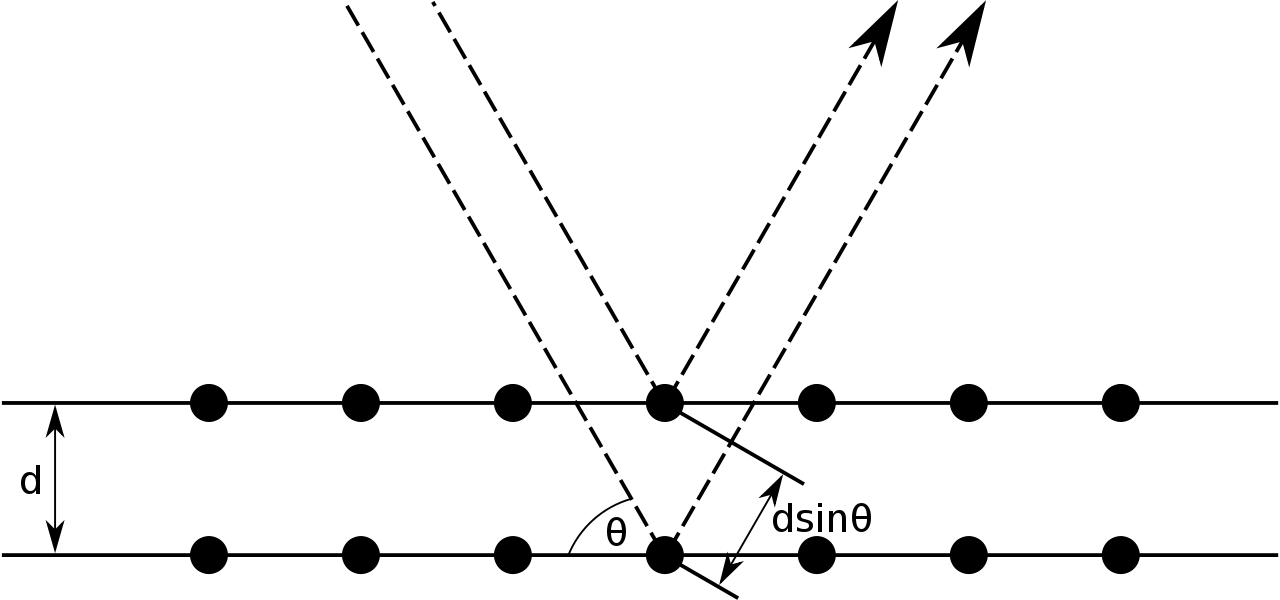
\includegraphics[scale=0.2]{./Images/Diagrams/1280px-BraggPlaneDiffraction.png} 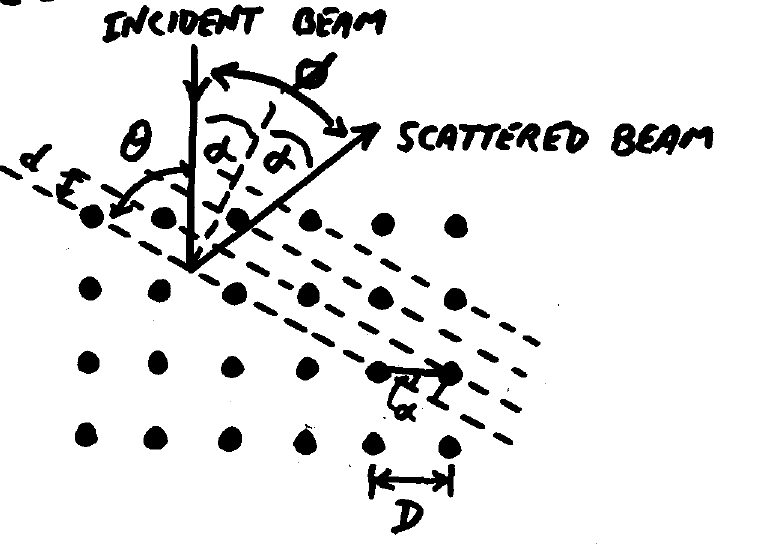
\includegraphics[scale=0.25]{./Images/Diagrams/crystalscattering.png}
\end{center}





The potential the electron moves in
\begin{align}
V(r)=\frac{-e^2}{(4\pi \epsilon_0r)}
\end{align}
The angular momentum of an electron in the atom
\begin{align}
L=mvr=\hbar\sqrt{\ell(\ell+1)} \\
L_z=m_\ell\hbar 
\end{align}
An electron orbiting around a nucleus has magnetic moment $\vec{\mu}$
\begin{align}
\vec{\mu}&=IA\hat{n}=\frac{-e}{(2\pi r/v)}(\pi r^2)\hat{n}=\frac{-erv}{2}\hat{n}=\frac{-e}{2m}\vec{L} \\
\mu_z&=\frac{-e}{2m}L_z=\frac{-e}{2m}m_l\hbar=-m_\ell\mu_B 
\end{align}
In an external magnetic field, $B$, the
magnetic dipole feels a torque $\vec{\tau}$ and has a potential energy $U_B$
\begin{align}
\vec{\tau}&=\vec{\mu}\times \vec{B} \\
V_B&=-\vec{\mu}\cdot \vec{B} = \frac{-e}{2m}\vec{L} \cdot \vec{B} \implies V_{Bz}= \mu_B m_\ell B_z
\end{align}


\newpage
\chapter{Quantum Mechanics}
\thispagestyle{fancy}
\begin{multicols}{2}
[Plane waves with electromagnetic wave frequencies and wavelengths]
	\noindent
	\begin{align}
		\psi(x,t) &=A\cos[2\pi(x-ct)/\lambda] \\
		c &= f \lambda \Longleftrightarrow f = \frac{c}{\lambda} \Longleftrightarrow \lambda = \frac{c}{f} \\
		T &=1/f \\
		\psi(x,t) &= A \cos(kx-\omega t) \\
		k &= 2\pi /\lambda \\
		\omega &= 2\pi f = 2 \pi /T
	\end{align}
	The energy in a photon (packet of light)
	\begin{align}
		E &=h f  = \frac{hc}{\lambda} = \hbar \omega \\
		dE &= -\frac{hc}{\lambda^2}d\lambda=-\frac{E^2}{hc}d\lambda \\ |\Delta \lambda | &= hc\frac{\Delta E}{E^2}
	\end{align}
\end{multicols}
The wave equation
\begin{align}
	\frac{1}{v^2}\frac{\partial^2 \psi}{\partial t^2} = \nabla^2\psi
\end{align}
A periodic wave can be constructed from a sum of plane waves
\begin{align}
	\psi(x,t) &= \sum_{i=1}^{n} A_i \cos(k_ix_i-\omega_i t) 
\end{align}
The \textbf{cubit}\index{Cubit} is defined as
\begin{align}
	|\psi\rangle &= c_1|1\rangle + c_0|0\rangle \\
	|\psi\rangle &= c_{11}|11\rangle+c_{01}|01\rangle+c_{10}|10\rangle+c_{00}|00\rangle \\
	&\vdots \nonumber
\end{align}
The quantum mechanical \textbf{expectation value} of an observable $\hat{X}$ in a normalized state $\psi$ is found by integrating over the entire space $\psi^*$ times the result obtained when the corresponding operator  acts on $\psi$. 
\begin{align}
	\langle \psi | \hat{X} | \psi \rangle = \int_{-\infty}^{\infty}\psi^* \hat{X}\psi dx
\end{align}
The state of the system is given by a wavefunction $\psi(\vec{r},t)$.  The probability density is the square modulus of the amplitude
\begin{align}
	P(\vec{r}) d\vec{r} = |\psi(\vec{r})|^2d\vec{r}
\end{align}
The probability of a particle being between $x_1$ and $x_2$ given a normalized wave function $\psi(x,t)$ is
\begin{align}
	P_{x\in x_1:x_2}(t)=\int_{x_1}^{x_2}|\psi(x,t)|^2dx=\int_{x_1}^{x_2} \psi^*(x,t)\psi(x,t) dx
\end{align}
The normalization of a wave function implies the probability over all space is 1.
\begin{align}
	P_{x\in -\infty:\infty}(t) = \int_{-\infty}^{\infty}|\psi(x,t)|^2dx=1
\end{align}
The \textbf{Schr\"{o}dingr Equation}\index{Schr\"{o}dingr Equation} is a partial differential equation that describes how the wavefunction of a physical system evolves over time. The (non-relativistic) Schr\"{o}dingr Equation for a particle moving in a 3-dimensional potential energy field $V(\vec{r})$ is
\begin{align}
	\hat{E}\psi(\vec{r},t) &= \frac{-\hbar^2}{2m} \nabla^2 \psi(\vec{r},t)+V(\vec{r})\psi(\vec{r},t)  \equiv \hat{H}\psi(\vec{r},t)
\end{align}
The general solution to the time-dependent \textbf{Schr\"{o}dingr Equation} is
\begin{align}
	\psi(\vec{r},t) = \sum c_n \psi_n(\vec{r})e^{-iE_n t/\hbar}.
\end{align}
\textbf{The Dirac equation}\index{Dirac equation}: the generalization of the time dependent Schr\"{o}dinger equation for the relativistically correct relationship between energy and momentum. It leads to negative energy states and antiparticles.
\begin{align}
	\bigg[\gamma^0mc^2+\sum_{i=1}^{3}\gamma^i\hat{p}_ic \bigg]\psi(\vec{r},t)=i\hbar\frac{\partial}{\partial t}\psi(\vec{r},t)
\end{align}
Each observable corresponds to a linear operator. A linear operator is something that acts on a state and gives another state.
The Hamiltonian operator is defined as the operator $\hat{H}$ such the energy $E$ of a system with wavefunction $\psi$ is an eigenvalue of $\hat{H}\psi$ or $\hat{H}\psi = E \psi$. 
\begin{align}
	\hat{H} &= \hat{K}+V(\hat{r}) = \frac{\hat{p}^2}{2m}+V(\hat{r})= \frac{-\hbar^2}{2m}\nabla^2	+V(\vec{r})
\end{align}
The Energy operator
\begin{align}
	i\hbar\frac{\partial \psi}{\partial t}=i\hbar\frac{\partial}{\partial t}Ae^{i(kx-\omega t)}=i\hbar(-i\omega)\psi&=\hbar\omega\psi=E\psi \implies\hat{E} = i\hbar \frac{\partial}{\partial t} \\
	\langle\psi| E |\psi \rangle = \int_{-\infty}^{\infty} \psi^* \hat{E} \psi dx &= i\hbar \int_{-\infty}^{\infty} \psi^* \frac{\partial \psi}{\partial t} dx
\end{align}
The operator for a particles kinetic energy is
\begin{align}
	\hat{K}&=\frac{-\hbar^2}{2m}\nabla^2 \\
	\hat{K}\psi = \frac{1}{2m}\hat{p}^2\psi &= \frac{1}{2m}\bigg(-i\hbar\frac{\partial}{\partial x}\bigg)^2\psi = \frac{-\hbar^2}{2m}\frac{\partial^2}{\partial x^2}\psi \\
	\langle\psi| \hat{K}|\psi \rangle = \int_{-\infty}^{\infty}\psi^*\hat{K}\psi dx &= \int_{-\infty}^{\infty}\psi^*\frac{1}{2m}\hat{p}^2\psi dx = \frac{-\hbar^2}{2m}\int_{-\infty}^{\infty}\psi^*\frac{\partial^2}{\partial x^2}\psi dx
\end{align}
The momentum operator
\begin{align}
	\hat{p}&\equiv-i\hbar\nabla = \frac{\hbar}{i}\nabla \\
	\frac{\partial \psi}{\partial x}=\frac{\partial}{\partial x}Ae^{i(kx-\omega t)}=ik\psi&=\frac{ip}{\hbar}\psi \implies\hat{p} = -i\hbar \frac{\partial}{\partial x} \\
	\langle\psi| \hat{p}|\psi \rangle = \int_{-\infty}^{\infty} \psi^* \hat{p} \psi dx &= -i\hbar \int_{-\infty}^{\infty} \psi^* \frac{\partial \psi}{\partial x} dx
\end{align}
The wave function solution for a particle confined to an infinite potential well with walls at $x=0$ and $x=a$ is as follows, with the corresponding energy eigenvalues (with $n\in\mathbb{N}$)
\begin{align}
	\psi(x) &=
	\begin{cases}
		\sqrt{\frac{2}{a}}\sin\left(\frac{n\pi x}{a}\right) &  0\leq x \leq a\\
		0 &  \textrm{ otherwise }
	\end{cases} \\
	E_n &=\frac{\hbar^2\pi^2}{2ma^2}n^2
\end{align}
The solution to The Schr\"{o}dingr Equation for a finite potential well with the potential
\begin{align}
	V(x)=
	\begin{cases}
		\infty & \textrm{ for } x<0 \\
		0 & \textrm{ for } 0 \leq x \leq a \\
		V_1 & \textrm{ for } x>a
	\end{cases}
\end{align}
with $E>V_1$ is
\begin{align}
	\psi(x) &=
	\begin{cases}
		0 & \textrm{ for } x<0 \\
		D\sin(kx) & \textrm{ for } 0 \leq x \leq a \\
		F\cos(k'x)+G\sin(k'x) & \textrm{ for } x>a
	\end{cases} \\
	& \textrm{ with } k'=\sqrt{k^2-\frac{2mV_1}{\hbar^2}}
\end{align}
with $E<V_1$ is
\begin{align}
	\psi(x) &=
	\begin{cases}
		0 & \textrm{ for } x<0 \\
		D\sin(kx) & \textrm{ for } 0 \leq x \leq a \\
		Fe^{-\gamma x} & \textrm{ for } x>a
	\end{cases} \\
	& \textrm{ with } \gamma^2=\frac{2m(V_1-E)}{\hbar^2}=\frac{2mV_1}{\hbar^2}-k^2
\end{align}
The solutions for a finite barrier (with the probability of reflection as $R=|B|^2/|A|^2$ and the probability of transmission as $T=|F|^2/|A|^2$) are
\begin{align}
	\psi_1&=Ae^{ikx}+Be^{-ikx} \hspace{1cm}\textrm{(incident + reflected)} \\
	\psi_2&=Ce^{ik'x}+De^{-ik'x} \hspace{1cm}\textrm{(intermediate)}\\
	\psi_3&=Fe^{ikx} \hspace{1cm}\textrm{(transmitted)} \\
	k&=\sqrt{2mE/\hbar^2}\\
	k'&=\sqrt{2m(E-U_0)/\hbar^2}
\end{align}
For any two Hermitian operators $A$ and $B$,
\begin{align}
	\Delta A \Delta B \geq \frac{1}{2}| \langle i [A, B] \rangle |
\end{align}
Atomic quantum numbers
\begin{align}
	n &= \textrm{ Principle Quantum Number } [n \in \mathbb{N}]\\
	\ell &= \textrm{ Orbital Angular Momentum Quantum Number } [\ell \in \mathbb{N}\union\{0\}, \ell < n] \\
	m_\ell &= \textrm{ Magnetic Quantum Number }[m_\ell \in [-\ell, \ell], m_\ell \in \mathbb{Z}]
\end{align}
\section{Simple Harmonic Oscillator\index{Harmonic oscillator}}
For a simple harmonic oscillator\index{Harmonic oscillator}, the potential energy is given by
\begin{align}
	V(x)&=\frac{1}{2}kx^2=\frac{1}{2}m\omega^2x^2\implies k=m\omega^2 \Longleftrightarrow \omega=\sqrt{\frac{k}{m}} 
\end{align}
The energies and wave functions are then given by
\begin{align}
	\psi_n & = \frac{1}{\sqrt{n!}}(a_+)^n\psi_0 \hspace{1.5cm} \psi_0(x) = \left(\frac{m\omega}{\pi \hbar}\right)^{1/4}e^{-\frac{m\omega}{2\hbar}x^2}  \\ E_n&=\left(n+\frac{1}{2}\right)\hbar\omega=\left(n+\frac{1}{2}\right)\hbar\sqrt{\frac{k}{m}}=\left(n+\frac{1}{2}\right)\frac{\hbar}{x}\sqrt{\frac{2V(x)}{m}}
\end{align}
The eigenfunctions, raising, and lowering operators are related to the eigenstates/vectors by
\begin{align}
	a_\pm = \frac{1}{ \sqrt{2\hbar m\omega} }(\mp i p + m\omega x), \hspace{1cm}
	H | n \rangle &= E_n |n \rangle, \hspace{1cm} H = \hbar \omega \left(a^\dagger a + \frac{1}{2}\right), \hspace{1cm}[a,a^\dagger]=1 \\	
	|n\rangle = \frac{(a^\dagger)^n|0\rangle}{\sqrt{n!}}, \hspace{1cm} a^\dagger|n\rangle \equiv a_+|n \rangle &= \sqrt{n+1}|n+1\rangle, \hspace{1cm} a|n \rangle \equiv a_-|n \rangle = \sqrt{n}|n-1\rangle
\end{align}
For the harmonic oscillator, x and p can be expressed in terms of the raising and lowering operators
\begin{align}
	x = \sqrt{\frac{\hbar}{2m\omega}}(a_++a_-) \hspace{2cm} p =i\sqrt{\frac{\hbar m \omega}{2}}(a_+-a_-).
\end{align}
\section{Spherical Harmonics}
The normalized angular wave functions are called \textbf{spherical harmonics}\index{Spherical harmonics} and are given by
\begin{align}
	Y_\ell^m(\theta,\phi) = \epsilon\sqrt{\frac{(2\ell+1)}{4\pi}\frac{(\ell-|m|)!}{(\ell+|m|)!}}e^{im\phi}P_\ell^m(\cos\theta), \hspace{1cm} \textrm{with} \hspace{1cm}\epsilon = \begin{cases} (-1)^m & m \geq 0 \\ 1 & m < 0 \end{cases}.
\end{align}
The \textbf{spherical harmonics} are automatically orthogonal so,
\begin{align}
	\int_0^{2\pi}\int_0^\pi[Y_\ell^m(\theta,\phi)]^*[Y_{\ell'}^{m'}(\theta,\phi)]\sin\theta d\theta d\phi=\delta_{\ell \ell'}\delta_{m m'}
\end{align}
The normalized \textbf{hydrogen wave functions} containing the quantum numbers $n, m,$ and $\ell$ are
\begin{align}
	\Psi_{n\ell m}(r,\theta,\phi) = \sqrt{\left(\frac{2}{na}\right)^3\frac{(n-\ell-1)!}{2n[(n+\ell)!]^3}}e^{-r/na}\left(\frac{2r}{na}\right)^\ell\left[L_{n-\ell-1}^{2\ell+1}(2r/na)\right]Y_{\ell}^{m}(\theta,\phi).
\end{align}
The ground state wave functions and energy of Hydrogen is
\begin{align}
	\Psi_{100}(r,\theta,\phi) = \frac{1}{\sqrt{\pi a^3}}e^{-r/a} \andspace{1cm} E_1 = -\left[\frac{m}{2\hbar^2}\left(\frac{e^2}{4\pi\epsilon_0}\right)^2\right] = -13.6 eV
\end{align}
Each operator $\hat{Y}$ has a set of eigenvalues y which are the possible values you can get on doing a measurement of Y. Each eigenvalues y is associated with an eigenstate $\phi_y(x)$ which is the state for which the values of Y is exactly y with no uncertainty. You can find the eigenstates and eigenvalues of an operator by 
\begin{align}
	\hat{Y}\phi_y(x) = y \phi_y(x).
\end{align}
The eigenstates of any operator $\hat{Y}$ form a complete orthonormal basis of states so we can write any state $\psi(x)$ in terms of them.
\begin{align}
	\psi(x) \equiv \sum_{y}A_y\phi_y(x) \hspace{0.5cm}\textrm{or}\hspace{0.5cm} \psi(x) \equiv \int A(y)\phi_y(x)dy.
\end{align}
To solve for the coefficients in the above expression we can use Fouriers trick, or
\begin{align}
	A(y) = \int \phi_y^*(x)\psi(x)dx 	
\end{align}
If you are within operator space you can find the expectation value of an operator by
\begin{align}
	\langle \hat{y} \rangle = \int y |A(y)|^2 dy.
\end{align}
The commutation relation is a relationship between two operators and given by
\begin{align}
	[x,y] \equiv xy-yx &\implies [x,y] = -[y,x] \\
	[x,y]=[y,x]=0 &\implies \textrm{$x$ and $y$ commute} \\
	[xy,z] = x[y,z]+[x,z]y \hspace{1cm} &\textrm{and} \hspace{1cm}[x,yz] = y[x,z]+[x,y]z.adv
\end{align} 
Position and momentum are related via commutation by the following:
\begin{align}
	[x,p_x]=[y,p_y]=[z,p_z]=i\hbar \\
	[x,p_y]=[x,p_z]=[y,p_x]=[y,p_z]=[z,p_x]=[z,p_y]=0.
\end{align} 
\section{Angular Momentum and Spin}
The angular momentum operators are related via commutation by the following:
\begin{align}
	[L_x,L_y]=i\hbar L_z \andspace{1cm} &[L_y,L_z]=i\hbar L_x \andspace{1cm} [L_z,L_x]=i\hbar L_y \\
	[L_x,\vec{r}]=i\hbar (z-y) \andspace{1cm} &[L_x,\vec{L}] = i\hbar (L_z-L_y) \andspace{1cm} [L_x,\vec{p}] = i\hbar(p_z-p_y) \\
	[\vec{L}^2,L_\pm]=0 \andspace{1cm}&[\vec{L}^2,L_z] = 0 \andspace{1cm} [L_z,L_\pm]=\pm \hbar L_\pm
\end{align}
The angular momentum operators as well as the raising and lowering operators are given by
\begin{align}
	\vec{L} &= \frac{\hbar}{i}\left(\hat{\phi}\frac{\partial}{\partial \theta}- \frac{\hat{\theta}}{\sin \theta}\frac{\partial}{\partial \phi}\right) \hspace{1cm} \textrm{and} \hspace{1cm} L_z =\frac{\hbar}{i} \frac{\partial}{\partial \phi}\\
	L_x &= \frac{L_++L_-}{2}= \frac{\hbar}{i}\left(-\sin\phi \frac{\partial}{\partial \theta}-\cot\theta \cos \phi \frac{\partial}{\partial \phi}\right) \\  L_y &= \frac{L_+-L_-}{2i}= \frac{\hbar}{i}\left(\cos\phi \frac{\partial}{\partial \theta}-\cot\theta \sin \phi \frac{\partial}{\partial \phi}\right) \\
	L_{\pm} &= L_x\pm i L_y = \pm \hbar e^{\pm i \phi} \left(\frac{\partial}{\partial \theta}\pm  i \cot(\theta)\frac{\partial}{\partial \phi}\right) \\
	\vec{L}^2 &= L_x+L_y+L_z =-\hbar^2 \left[\frac{1}{\sin\theta}\frac{\partial}{\partial \theta}\left(\sin\theta\frac{\partial }{\partial \theta}\right)+\frac{1}{\sin^2\theta}\frac{\partial^2}{\partial \phi^2}\right]
\end{align}
The angular momentum operators satisfy
\begin{align}
	\vec{L}^2 | \ell, m \rangle = \hbar^2\ell(\ell+1)| \ell, m \rangle \andspace{1cm} L_z| \ell, m \rangle = \hbar m | \ell, m \rangle \\
	L_{\pm} | \ell, m \rangle = \hbar \sqrt{(\ell \mp m)(\ell \pm m +1)} | \ell, m \pm 1 \rangle
\end{align}
The fundamental commutation relations for spin are
\begin{align}
[S_x,S_y]=i\hbar S_z \andspace{1cm} [S_y,S_z]=i\hbar S_x \andspace{1cm} [S_z,S_x]=i\hbar S_y.
\end{align}
The general state of a spin-1/2 particle can be expressed as a two element column matrix (or spinor):
\begin{align}
\chi= \begin{pmatrix}
a\\b
\end{pmatrix} = a \begin{pmatrix}
1\\0
\end{pmatrix}+b\begin{pmatrix}
0\\1
\end{pmatrix}= a \chi_++b\chi_-.
\end{align}
The spin matrices are given by
\begin{align}
\vec{S}_x &= \frac{\hbar}{2}\begin{pmatrix}
0 & 1 \\ 1 & 0
\end{pmatrix}, \hspace{1cm}\vec{S}_y = \frac{\hbar}{2}\begin{pmatrix}
0 & -i \\ i & 0
\end{pmatrix}, \hspace{1cm}\vec{S}_z = \frac{\hbar}{2}\begin{pmatrix}
1 & 0 \\ 0 & -1
\end{pmatrix}, \\ \vec{S}_+ &= \hbar\begin{pmatrix}
0 & 1 \\ 0 & 0
\end{pmatrix}, \hspace{1cm}\vec{S}_- = \hbar\begin{pmatrix}
0 & 0 \\ 1 & 0
\end{pmatrix}, \hspace{1.3cm}\vec{S}^2 = \frac{3\hbar^2}{4}\begin{pmatrix}
1 & 0 \\ 0 & 1
\end{pmatrix}
\end{align}
The \textbf{Pauli Spin Matrices}\index{Pauli Spin Matrices} are then given by
\begin{align}
\sigma_x \equiv \begin{pmatrix}
0 & 1 \\ 1 & 0
\end{pmatrix}, \hspace{1cm}\sigma_y \equiv \begin{pmatrix}
0 & -i \\ i & 0
\end{pmatrix}, \hspace{1cm}\sigma_z \equiv \begin{pmatrix}
1 & 0 \\ 0 & -1
\end{pmatrix}
\end{align}
The combined state $| s, m \rangle$  with total spin s and z-component m will be some linear combination of the composite states $| s_1, m_1 \rangle$ and $| s_2, m_2 \rangle$ and depends on the Clebsch-Gordan\index{Clebsch-Gordan} Coefficients $C_{m_1m_2m}^{s_1s_2s}$ (page \pageref{Clebsch-Gordan}):
\begin{align}
| s, m \rangle = \sum_{m=m_1+m_2} C_{m_1m_2m}^{s_1s_2s}| s_1, m_1 \rangle| s_2, m_2 \rangle, \hspace{1.5cm} | s_1, m_1 \rangle| s_2, m_2 \rangle = \sum_{s} C_{m_1m_2m}^{s_1s_2s}| s, m \rangle
\end{align}

\begin{fancybox}[Hund's Rules]{}
To find the state with the lowest energy configuration,
	\begin{enumerate}
		\item Choose the largest S.
		\item Choose the Largest L (consistent with the Pauli Exclusion Principle).
		\item If the shell is less than one half filled, choose the smallest J. If the shell is greater than one half filled, choose the largest J. If the shell is half filled, then $L=0 \implies J=S$.
	\end{enumerate}
\end{fancybox}

From the \textbf{Time-independent perturbation theory} at an approximation gives the correction energy ($1^{st}$ and $2^{nd}$ order given) and wave function ($1^{st}$ order) as
\begin{align}
	| \psi_n^{(1)} \rangle = \sum_{\ell \neq n} | \psi_\ell^{(0)} \rangle \frac{\langle \psi_\ell^{(0)}|H^1| \psi_n^{(0)} \rangle }{E_n^{(0)}-E_\ell^{(0)}} \hspace{1cm} E_n^{(1)}=\langle \psi_n^{(0)}|H^1| \psi_n^{(0)}\rangle  \hspace{1cm} E_n^{(2)} = \sum_{m \neq n} \frac{|\langle \psi_m^{(0)}|H^1| \psi_n^{(0)} \rangle|^2 }{E_n^{(0)}-E_m^{(0)}}  
\end{align}

The \textbf{variational principle}\index{Variational principle} will give an upper bound for the ground state energy for a system described by the Hamiltonian H. This is often useful when you are unable to solve Schr\"{o}dinger's equation.
\begin{align}
	E_{gs} \leq \langle \psi|H|\psi\rangle
\end{align}

\newpage
\chapter{Nuclear and High Energy Physics}
\thispagestyle{fancy}
\section{Nuclear Physics}
The atomic nucleus consists of protons and neutrons collectively called nucleons. Nuclei with different number of neutrons but with the same number of protons are isotopes of the same element. The mass number of an isotope os the sum of the number of protons (Z) and the number of neutrons (N)
\begin{align}
A=Z+N.
\end{align}
Nuclei are approximately spherical in shape, with the radius of the sphere depending on the mass number ($R_0=1.12$ fm)
\begin{align}
R(A)=R_0A^{1/3}.
\end{align}
The nucleon density in the interior of a nucleus is $n=0.17$ fm$^{-3}$, and the mass density is $\rho=m_{nucleon}n=2.8\times 10^{17}$kg/m$^3$. The dependence of the density on the radial coordinate is given by the Fermi function ($a=0.54$ fm):
\begin{align}
n(r)=\frac{n_0}{1+e^{(r-R(A))/a}}.
\end{align}
The Nuclear (or ``strong'') force\index{Nuclear Force} is what binds the protons and neutrons together into nuclei with the following properties:
\begin{enumerate}[(i)]
	\item Within the nucleus, it is about 100 times stronger than the electromagnetic force and approximately $10^{38}$ times stronger than gravity.
	\item It is charge-independent.
	\item It is spin-dependent.
\end{enumerate}
In any nuclear reaction, the following quantities are conserved: 
\begin{center}
	Nuclean Number (A), electric charge, total energy and total momentum.
\end{center}
The mass of a nucleus with Z protons and N neutrons is smaller than the sum of the individual nucleon masses, and the binding energy is defined as the mass difference times $c^2$:
\begin{align}
B(N,Z)=Zm(0,1)c^2+Nm_nc^2-m(N,Z)c^2.
\end{align}
The \textbf{mass excess} of a nucleus is defined as the difference between the mass of a nucleus expressed in atomic mass units and the mass number:
\begin{align}
\textrm{mass excess}=m(N,Z)-(A)(1 u).
\end{align} 
The binding energies of different isotopes can be reproduced well by the Bethe-Weizs\"{a}cher formula from the liquid-drop model, as the sum of volume, surface, Coulomb, asymmetry, and pairing contributions:
\begin{align}
B(N,Z)&=B_v(N,Z)+B_s(N,Z)+B_c(N,Z)+B_a(N,Z)+B_p(N,Z) \\
&=a_vA-a_sA^{2/3}-a_cZ^2A^{-1/3}-a_a\bigg(Z-\frac{1}{2}A \bigg)^2A^{-1}+a_p\big((-1)^Z+(-1)^N \big)A^{-1/2}.
\end{align}
Dividing this expression by the mass number gives the binding energy per nucleon:
\begin{align}
\frac{B(N,Z)}{A}=a_v-a_sA^{-1/3}-a_c\frac{Z^2}{A^{4/3}}-a_a\bigg(\frac{Z}{A}-\frac{1}{2} \bigg)^2+a_p\frac{(-1)^Z+(-1)^N}{A^{3/2}}.
\end{align}
Several successful fits have been published for the empirical mass formula above. Using the values obtained by Bertulani and Schechter (2002), we have
\begin{center}
	$a_v=15.85$ MeV, $a_s=18.34$ MeV, $a_c=0.71$ MeV, $a_a=92.86$ MeV, $a_p=11.46$ MeV. 
\end{center}
The Fermi gas model proposes a quantum gas of nucleons that can move freely inside the nucleus but are confined by the nuclear surface. The density of states in the Fermi gas model is 
\begin{align}
dN(E)=\frac{1}{\pi^2 a^3\hbar^3}\sqrt{\frac{m^3E}{2}}dE.
\end{align}
The \textbf{Fermi energy}\index{Fermi energy} is
\begin{align}
E_F=\frac{\hbar^2}{2m}\sqrt[3]{\frac{9}{4}\pi^4n_0^2}=38 \textrm{ MeV}.
\end{align}
In a nuclear reaction, the difference between final and initial
kinetic energies is called the $Q$-value:
\begin{align}
Q&=\Delta KE=-\Delta Mc^2 \hspace{1cm}
\begin{cases}
Q>0 \implies \textrm{Exothermic} \\
Q<0 \implies \textrm{Endothermic}
\end{cases}
\end{align}







\section{Nuclear Decay}
\begin{multicols}{2}
Nuclear decays\index{Nuclear Decay} follow an exponential decay law. The decay constant $\lambda$, half life $t_{1/2}$, and mean lifetime $\tau$ are related:
\begin{align}
N(t)&=N_0e^{-\lambda t}\\
t_{1/2}&=\frac{\ln(2)}{\lambda}=\tau \ln(2).
\end{align}
In alpha ($\alpha$) decay, a heavier nucleus (Nuc) emits a helium-4 nucleus:
\begin{align}
{}^A_Z\textrm{Nuc} \to {}^{4}_{2}\textrm{He} + {}^{A-4}_{Z-2}\textrm{Nuc'}
\end{align}
In a $\beta^-$ decay, an electron and an anti-neutrino are emitted:
\begin{align}
{}^A_Z\textrm{Nuc} \to {}^{A}_{Z+1}\textrm{Nuc'} + e^- +\bar{v}_e
\end{align}
In a $\beta^+$ decay can proceed via a positron emission:
\begin{align}
{}^A_Z\textrm{Nuc} \to {}^{A}_{Z-1}\textrm{Nuc'} + e^+ +v_e
\end{align}
This type of decay can also occur via electron capture
\begin{align}
e^-+{}^A_Z\textrm{Nuc} \to {}^{A}_{Z-1}\textrm{Nuc'} +v_e
\end{align}
A \textbf{gamma decay}\index{Gamma decay} is an emission of a high-energy photon from an excited nucleus, a process that does not transmute the nucleus:
\begin{align}
{}^A_Z\textrm{Nuc} \to {}^{A}_{Z}\textrm{Nuc'} +\gamma
\end{align}
\end{multicols}



\section{Elementary Particle Physics}
Substructure is probed using scattering experiments. The scattering cross section is defined as
\begin{align}
\sigma = \frac{\textrm{\# of reactions per scattering center/s}}{\textrm{\# of impinging particles/s/m$^2$}}.
\end{align}
The scattering cross section has the physical dimension of area and is measured in the unit barn (b) or millibarn (mb):
\begin{align}
1 \textrm{ b} &= 10^{-28} \textrm{ m}^2\hspace{1cm}\textrm{and}\hspace{1cm}
1 \textrm{ mb} = 10^{-31} \textrm{ m}^2.
\end{align}
The classical \textbf{Rutherford cross section}\index{Rutherford cross section} for scattering from a pointlike target by the Coulomb interaction is
\begin{align}
\frac{d \sigma}{d \Omega}=\bigg(\frac{kZ_PZ_te^2}{4K} \bigg)^2\frac{1}{\sin^4(\theta/2)}.
\end{align}
For scattering of a plane wave off a point source, the scattering wave function is
\begin{align}
\psi_{total}(\vec{r})&=\psi_i(\vec{r})+\psi_f(\vec{r})
=N\bigg(e^{ikz}+f(\theta)\frac{e^{ikr}}{r} \bigg) \hspace{1cm}\textrm{and}\hspace{1cm}
\frac{d \sigma}{d \Omega}=|f(\theta)|^2.
\end{align}
The form factor is the Fourier transform of the density distribution and measures the deviation of the scattering cross section from the Rutherford cross-section of a point-like target:
\begin{align}
F^2(\Delta p)&= \bigg|\frac{1}{e}\int\rho(\vec{r})e^{i\Delta \vec{p} \cdot \vec{r}/\hbar}dV\bigg|^2\hspace{1cm}\textrm{and}\hspace{1cm}
\frac{d \sigma}{d \Omega}= \bigg(\frac{d \sigma}{d \Omega} \bigg)_{point} \cdot F^2(\Delta p).
\end{align}
\begin{itemize}
	\item Elementary fermions have spin $\frac{1}{2}\hbar$ and include the six quarks (up, down, strange, charm, bottom, and top), the electron, muon, and tau leptons, and the electron-, muon-, and tau-neutrinos. Each of these 12 fermions has an antiparticle. Quarks all have a non-integer charge of $-\frac{1}{3}e$ or $+\frac{2}{3}e$ and cannot be observed in isolation.
	\item Elementary bosons are the mediators of the interactions between the fermions. They are the photon (electromagnetic), the W and Z bosons (electroweak), the gluon (strong), and the graviton (gravitational). The graviton is yet to be found experimentally. Gluons can also interact with other gluons. 
	\item Elementary quarks and antiquarks can combine to form color singlets, which are particles that can be observed in isolation. A quark and an antiquark can form a meson (pion, kaon, etx.). Three quarks can form a baryon (proton, neutron, delta baryon, etc.). The only stable baryon is the proton, and none of the mesons is stable. Lifetimes of the unstable particles vary from $10^{-23}$ seconds to 15 minutes.
	\item The quark-gluon plasma phase transition of the early universe can be probed in the laboratory with relativistic heavy ion collisions. The primordial fraction of 23\% helium in the universe can be explained from the neutron-proton mass difference, which fixes the ratio of proton and neutron numbers to $n_n/n_p = e^{(m_n-m_p)c^2/k_BT}$.
\end{itemize}
Single and double nucleon separation energies\index{Separation energy} ($S_{n_1}$ and $S_{n_2}$) are given by
\begin{align}
	S_{n_1} &= B(N,Z)-B(N-1,Z) \andspace{1cm} S_{n_2} = B(N,Z)-B(N-2,Z) \\
	S_{p_1} &= B(N,Z)-B(N,Z-1) \andspace{1cm} S_{p_2} = B(N,Z)-B(N,Z-2).
\end{align}
The neutron pairing gap as related to the separation energies is given by
\begin{align}
\Delta_{n} = \frac{(-1)^N}{2} \left[S_{n_1}(N,Z)-S_{n_1}(N-1,Z)\right].
\end{align}


\newpage
\chapter{Advanced Physics}
\thispagestyle{fancy}
\section{Quantum Chromodynamics}
The classical Lagrangian density for $n$ non-interacting quarks with masses $m_i$ is 
\begin{align}
\mathcal{L}_{\textrm{quarks}}=\sum_{i}^{n}q_i^{-a}(i\eth-m_i)_{ab}a_i^b.
\end{align}
The Quantum Chromodynamic Lagrangian is given by
\begin{align}
\mathcal{L}_{\textrm{QCD}}=-\frac{1}{4}F^A_{\mu\nu}F^{\mu\nu}_A+\sum_{i}^{n}q_i^{-a}(i\eth-m_i)_{ab}a_i^b-\frac{1}{2\lambda}(\partial^\mu A^A_\mu)^2+\mathcal{L}_{\textrm{ghost}}.
\end{align}
The Lagrange equation for a multiple pendulum system with n number of rods, where the $i^{th}$ rod has a length $L_i$, and mass $m_i$.
\begin{align}
\mathcal{L}&=\frac{1}{2}\sum_{i=1}^{n}m_i(\dot{x}^2_i+\dot{y}^2_i)+\frac{1}{6}\sum_{i=1}^{n}m_iL_i^2\dot{\theta}_i^2-g\sum_{i=1}^{n}m_iy_i.
\end{align}
The normalized hydrogen wave functions are:
\begin{align}
	\Psi_{n\ell m}(r,\theta,\phi) = \sqrt{\left(\frac{2}{na}\right)^3\frac{(n-\ell-1)!}{2n[(n+\ell)!]^3}}e^{-r/na}\left(\frac{2r}{na}\right)^\ell\left[L_{n-\ell-1}^{2\ell+1}(2r/na)\right]Y_{\ell}^{m}(\theta,\phi)
\end{align}





\unchapter{Resources}

\invisiblesection{Clebsch-Gordan Coefficients, spherical harmonics, and d functions.}

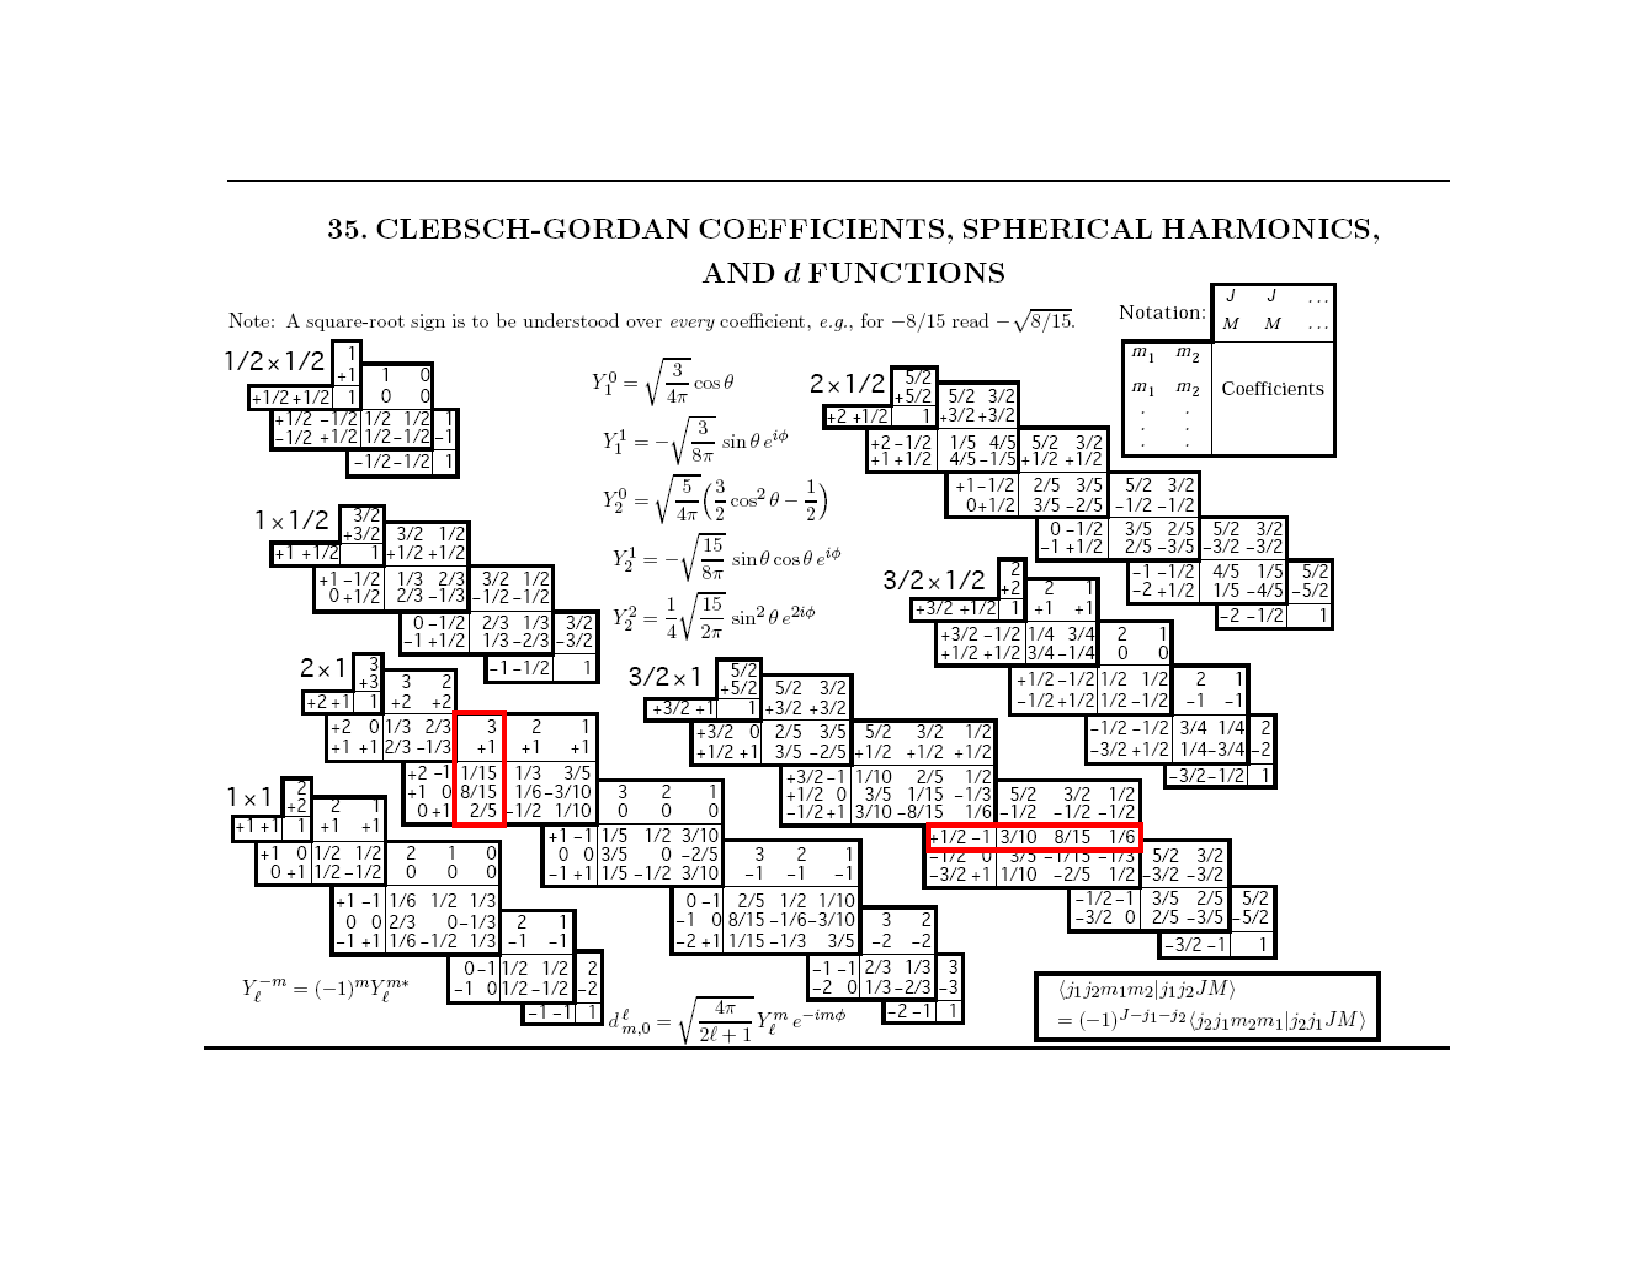
\includepdf[pages=1,angle=90,pagecommand=\thispagestyle{fancy}]{Resources/Clebsch-Gordan}

\invisiblesection{Table of Isotopic Masses and Natural Abundances}

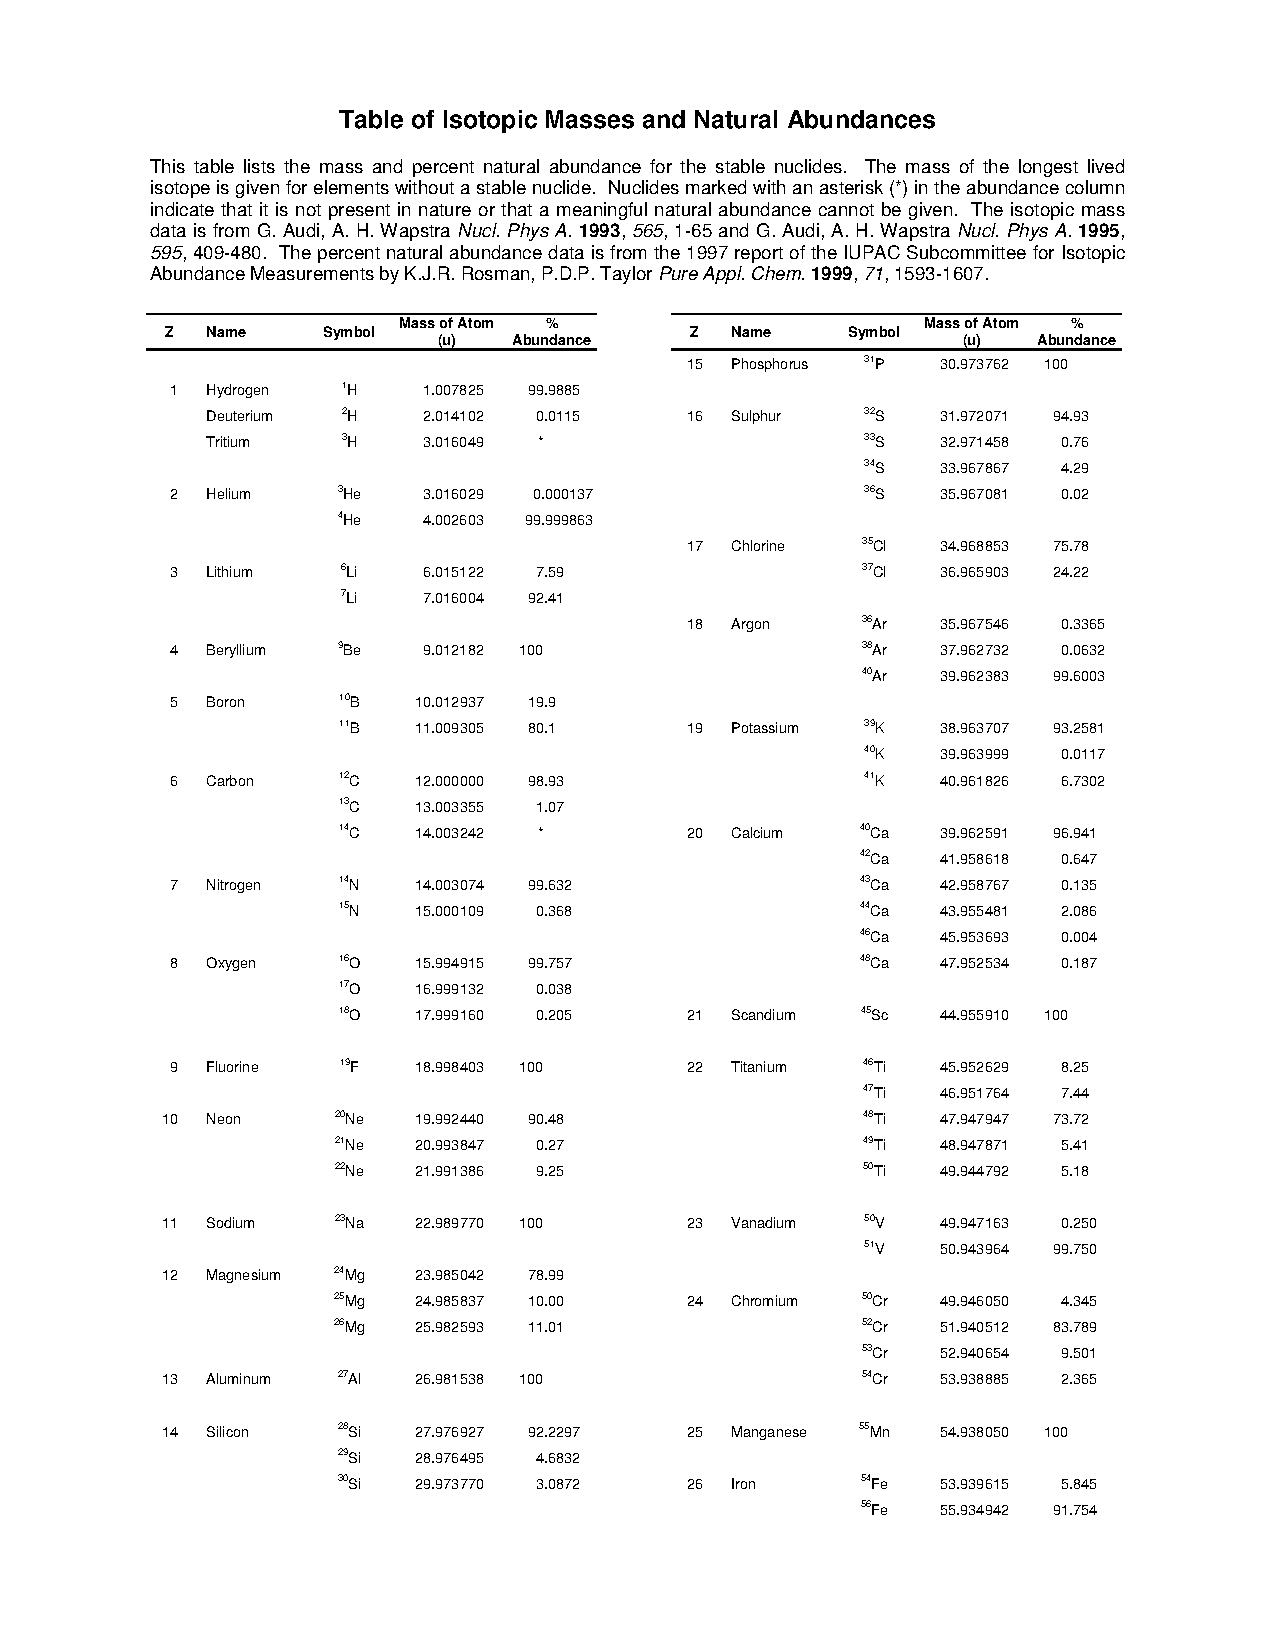
\includepdf[pages=1,pagecommand=\thispagestyle{fancy}]{Resources/IsotopicMassNaturalAbundance}
\includepdf[pages=2,pagecommand=\thispagestyle{fancy}]{Resources/IsotopicMassNaturalAbundance}
\includepdf[pages=3,pagecommand=\thispagestyle{fancy}]{Resources/IsotopicMassNaturalAbundance}
\includepdf[pages=4,pagecommand=\thispagestyle{fancy}]{Resources/IsotopicMassNaturalAbundance}
\includepdf[pages=5,pagecommand=\thispagestyle{fancy}]{Resources/IsotopicMassNaturalAbundance}

\invisiblesection{Periodic Table of Elements}

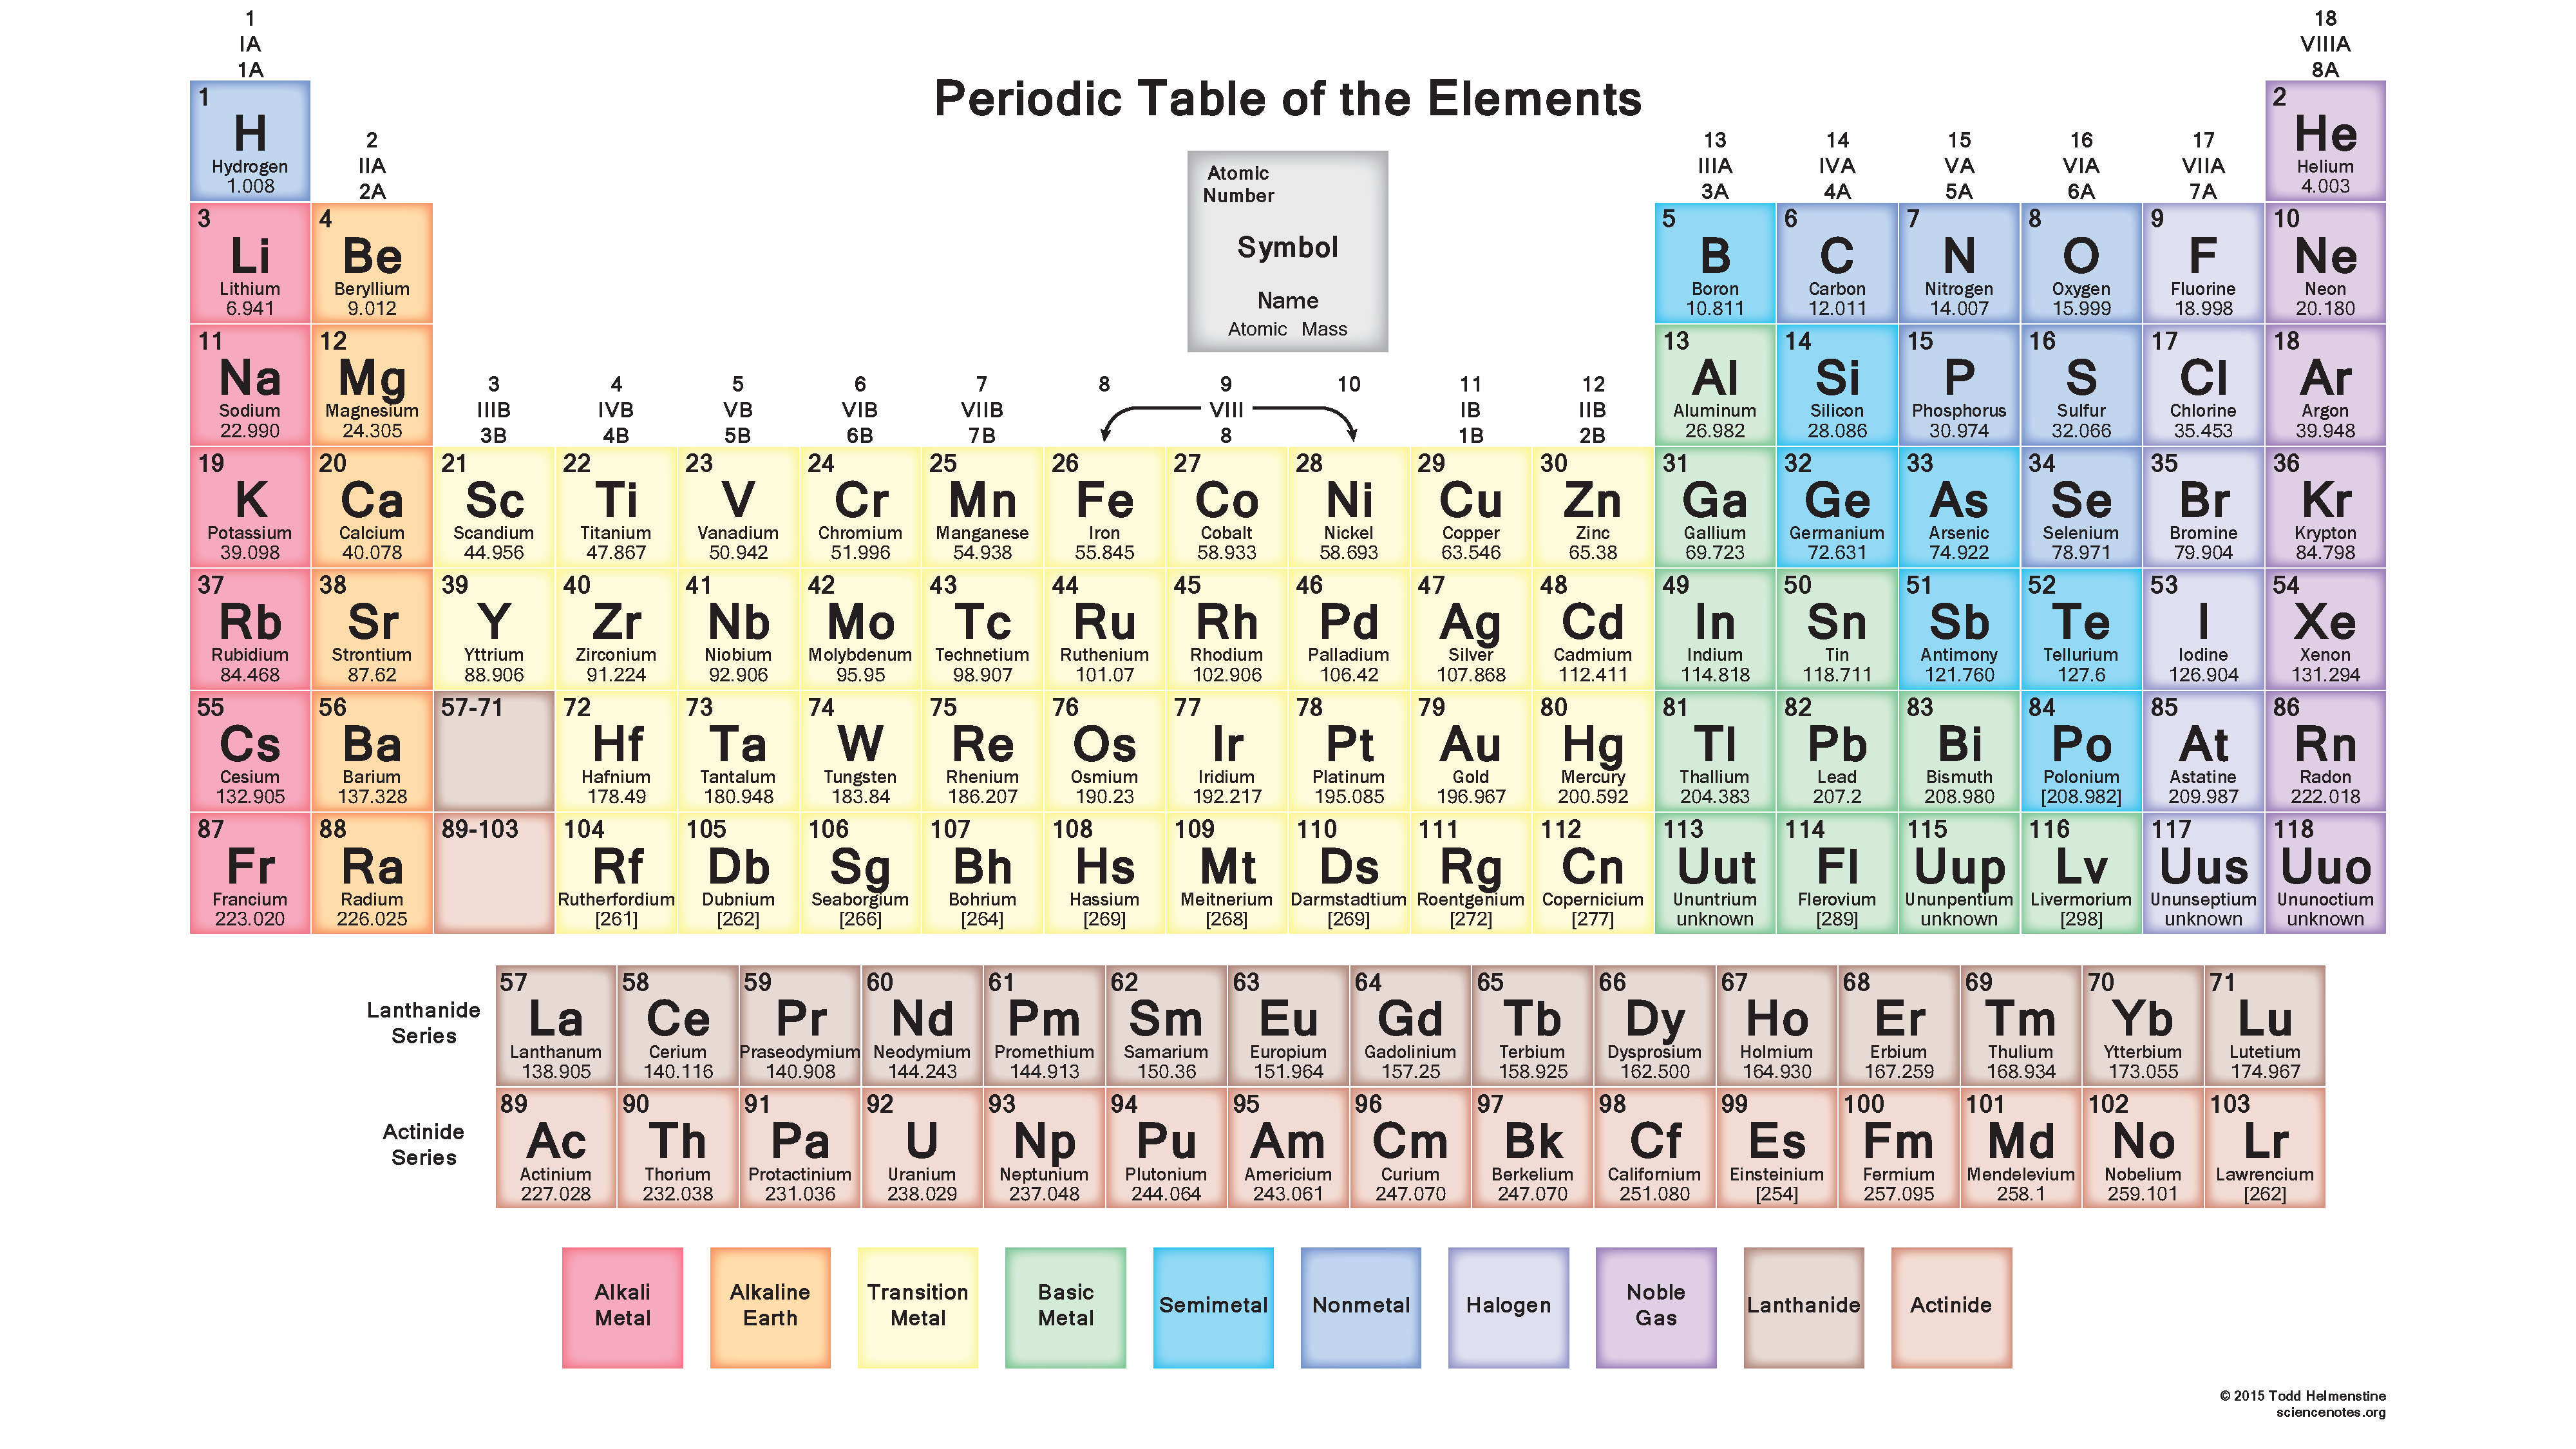
\includepdf[pages=1,angle=90,pagecommand=\thispagestyle{fancy}]{Resources/PeriodicTableMuted2}

%Begin the backmatter.
\backmatter
{\footnotesize
\begin{thebibliography}{99}
	\bibitem{bib:Modern_Physics} Bauer, W., and Gary D. Westfall. University Physics with Modern Physics. 2nd ed. Vol. 2. New York, NY: McGraw-Hill Companies, 2014. Print. 	
	
	\bibitem{bib:Methods_Of_Theoretical}Boas, Mary L. Mathematical Methods in the Physical Sciences. 3rd ed. New York: John Wiley \& Sons, 1984. Print. 
	
	\bibitem{bib:Planets_and_telescopes} Brown, Edward, comp. ``Planets And Telescopes." (2015): n. pag. Print. Michigan State University Department of Astronomy and Physics
	
	\bibitem{bib:AST304} Brown, Edward, comp. Astronomy 304 class handouts (2015): n. pag. Print. Michigan State University Department of Astronomy and Physics
	
	\bibitem{bib:StellarAstrophysics} Brown, Edward, comp. ``Stellar Astrophysics." (2015): n. pag. Print. Michigan State University Department of Astronomy and Physics
	
	\bibitem{bib:dictionary} http://www.dictionary.com
	
	\bibitem{bib:Griffiths} Griffiths, David J. Introduction to Electrodynamics. 4th ed. N.p.: Pearson India Education Services Pvt, 2015. Print. 
	
	\bibitem{bib:PeriodicTable} Helmenstine, Todd. Periodic Table of the Elements. sciencenotes.org. 2015.
	
	\bibitem{bib:Linnemann} Linnemann, Jim, Dr. Modern Physics Lecture Notes. 2016. PHY 215 lecture notes. Department of Physics and Astronomy, Michigan State University. 
	
	\bibitem{bib:AbstractNotes} Meierfrankenfeld, Ulrich. MTH 310 Lecture Notes Based on Hungerford, Abstract Algebra. N.p.: Department of Mathematics, Michigan State U, 2015. Print. 
	
	\bibitem{electronics} Plonus, Martin. Electronics and Communications for Scientists and Engineers. San Diego: Academic, 2001. Print. 
	
	\bibitem{bib:ReitzEMTheory} Reitz, John Richard. Foundations of Electromagnetic Theory. 4th ed. N.p.: Addison-Wesley, 1992. Print. 
	
	\bibitem{bib:Kittel_ThermalPhysics}  Kittel, Charles, and Herbert Kroemer. Thermal Physics. San Francisco: W.H. Freeman, 1980. Print.
	
	\bibitem{Nazarewicz_PHY802} Nazarewicz, Witek. "MSU PHY802 Lecture Slides." Survey of Nuclear Physics 802/492 Spring 2017. Michigan State University, n.d. Web. 31 Mar. 2017. 
	
	\bibitem{bib:Foundations_Of_Astrophysics} Ryden, Barbara Sue., and Bradley M. Peterson. Foundations of Astrophysics. San Francisco: Addison-Wesley, 2010. Print. 
	
	\bibitem{bib:elementTable} ``Table of Isotopic Masses and Natural Abundances." (n.d.): n. pag. NC State University. Web. ``https://www.ncsu.edu/chemistry/msf/pdf/IsotopicMass\_NaturalAbundance.pdf". 
	
	\bibitem{bib:Classical_Mechanics} Taylor, John R. Classical Mechanics. Sausalito, CA: U Science, 2005. Print. 
	
	\bibitem{bib:WolfrmAlpha} ``Wolfram$|$Alpha: Computational Knowledge Engine." N.p., n.d. Web. 2016 x
	
	\bibitem{bib:Wolfram} ``Wolfram MathWorld: The Web's Most Extensive Mathematics Resource." Wolfram MathWorld. N.p., n.d. Web. 
	
	\bibitem{DiffEQ} Zee, Dennis G. A first Course in Differential Equations with Modeling Applications." Edition 10. Book.
\end{thebibliography}
}


\end{document}